\documentclass[twoside,english]{uiofysmaster}
\usepackage{physics}
\usepackage[nottoc]{tocbibind}
\usepackage{tikz}
\usepackage[utf8]{inputenc}
\usepackage[T1]{fontenc}
%\usepackage{lmodern}
\usepackage{listingsutf8}
\usepackage{simplewick}
\usepackage{booktabs}
\usepackage{graphicx}
\usepackage{textcomp}
\usepackage{float}
\usepackage{grffile}
\usepackage{tabularx}
\usepackage[page]{appendix}


\makeatletter
\@ifundefined{showcaptionsetup}{}{%
 \PassOptionsToPackage{caption=false}{subfig}}
\usepackage{subfig}
\makeatother


\interfootnotelinepenalty=10000 % make footnotes stay in one page
\numberwithin{equation}{section} % give equations numbering for the section
\setlength{\parindent}{0em} % paragraph indentation
\setlength{\parskip}{1em} % paragraph spacing

\setlength\tabcolsep{1em} % table column spacing
\renewcommand{\arraystretch}{1.2} % table row spacing

% #################### Tikz settings ####################
\usetikzlibrary{shapes,arrows,chains,positioning}
% =================================================
% Set up a few colours
\colorlet{lcfree}{ForestGreen}
\colorlet{lcnorm}{MidnightBlue}
\colorlet{lccong}{Maroon}
% -------------------------------------------------
% Set up a new layer for the debugging marks, and make sure it is on
% top
\pgfdeclarelayer{marx}
\pgfsetlayers{main,marx}
% ########################################################
% ########################################################

% #################### Listings style ####################
\definecolor{dark-gray}{gray}{0.3}
\lstdefinestyle{liststyle}{
	%backgroundcolor=\color{backcolour},   
	commentstyle=\color{ForestGreen},
	keywordstyle=\color{blue},
	stringstyle=\color{cyan},
	basicstyle=\ttfamily\footnotesize,
	%breakatwhitespace=false,         
	%breaklines=true,                 
	%captionpos=b,                    
	%keepspaces=true,                 
	numbers=left,                    
	numbersep=12pt,    
	numberstyle=\footnotesize\color{dark-gray},              
	%showspaces=false,                
	%showstringspaces=false,
	%showtabs=false,                  
	tabsize=2,
	basewidth = {0.5em, 0.5em},
	columns = fullflexible,
	numberblanklines=false,
	escapeinside=||
}
\lstset{style=liststyle, aboveskip=10pt, belowskip=5pt}

\let\origthelstnumber\thelstnumber
\makeatletter

\newcommand*\Suppressnumber{%
  \lst@AddToHook{OnNewLine}{%
    \let\thelstnumber\relax%
     \advance\c@lstnumber-\@ne\relax%
    }%
}

\newcommand*\Reactivatenumber[1]{%
  \setcounter{lstnumber}{\numexpr#1-1\relax}
  \lst@AddToHook{OnNewLine}{%
   \let\thelstnumber\origthelstnumber%
   \refstepcounter{lstnumber}
  }%
}

\makeatother
% ########################################################
% ########################################################

\newcommand{\todo}[1]
{
	\Large
	\textsf{\textbf{\textcolor{Red}{TODO: #1}}}
	\normalsize	
}
\newcommand{\braVket}[3]
{
	\left\langle #1 \right | #2 \left | #3 \right\rangle
}

\begin{document}
	\author{H\aa kon Sebastian Bakke M\o rk}
	\title{\uppercase{Quantum Monte Carlo studies of Many-Electron systems}}
	\date{June 2016}

	\maketitle

	\begin{abstract}
	This is an abstract text.
	\end{abstract}

	\begin{dedication}
	  To someone
	  \\\vspace{12pt}
	  Dedications here.
	\end{dedication}

	\begin{acknowledgements}
	  Acknowledgements here.
	\end{acknowledgements}

	\tableofcontents{}
	%\clearpage
	%\listoffigures

	%\listoftables




	


Removing the basis incompleteness and finite size errors by formatting it as an extrapolation problem is a promising application of machine learning because it is well formatted. Furthermore, the extrapolations are known to have asymptotic values for the correlation energies (i.e., the converged values), there is a simple pattern in the data for the machine learning to pick up, and the training data is already near the converged values (but still far enough away that performing the extrapolation increases the accuracy of the results) \cite{Ref6}.

Attempting to remove basis incompleteness and finite size errors from many-body calculations with machine learning is not a novel idea. For example, in Ref \cite{Ref6}, the authors attempt to use a neural network to perform an extrapolation to remove the basis incompleteness error for a harmonic oscillator basis used in coupled cluster calculations of nuclei. However, the authors encountered the problems that would be expected when using neural networks for this application, including difficulty working with small data sets (leading to the need for interpolation before extrapolation) and neural network's inability to create exactly reproducible results due to its training process \cite{Ref6}. Another example of using machine learning to remove truncation errors from many-body calculations can be found in ADD MORE HERE. However, further examples can be found in Refs. \cite{ADD NUMBER} through \cite{ADD NUMBER}.

We should point out that other methods exist to eliminate the finite size errors other than performing calculations at higher N or extrapolating. One of these options is to use twisted boundary conditions instead of periodic boundary conditions, which provide much more accurate estimates of the correlation energies \cite{Ref4}.

	\part{Theory}
		\chapter{Scientific Computing}
			A great deal of problems cannot be solved using analytical
methods. And except for very simple problems, it is impossible to
find an analytical solution. For this reason scientific computing is a
rapidly growing field, and is now applied in a wide range of
fields. These include not only natural sciences and mathematics, but
also medicine, sociology, and economics to name a few. In physics, the
dawn of computational solution-methods gave rise to the field of
computational physics, and is today used in every major field from
astrophysics to quantum physics.

In essence scientific computing is taking a real world phenomena,
which often are chaotic and noisy, and making a model that is abstract
and perhaps simplified. The model is then used in an automated
simulation to solve the problem at hand. This means that the model has
to be implemented in a computer program and executed on a computer.

%\todo{Knytt til det som er viktig for oppgaven (Obj. or. gjør fleksibel; nyttig for bruk som her.)}

\section{Types of programming languages}
	A computer program contains a set of instructions to be
        executed by the computer. These are usually in the form of an
        algorithm, that is a series of instructions designed to solve
        a given problem, or perform a specific task.

	As with human languages there exists many different computer
        languages, such as Python, C++ or Java. However the machine is
        almost never able to perform the instructions written as they
        are\footnote{One exception is if the program is written in
          machine code, which can be executed (almost) directly by the
          processor. But writing a program in machine code is tiresome
          and error-prone, and is thus rarely done except in extreme
          cases.}.  To carry out the written instructions the program
        has to be compiled or interpreted, depending on the
        language. Using a compiler, the program is compiled in advance
        of execution and creates an executable program which can be
        run on the central processing unit (CPU). If the program is
        written in a scripted language, however, the code is fed to an
        interpreter at execution time, which processes the written
        instructions and carries them out on the CPU.

	It is well known that the native language of the computer is
        binary. In other words it is made up of ones and zeros called
        bits, corresponding to high and low voltage readings in the
        CPU. Everything from numbers to words to colors and so on is
        represented in the computer as a sequence of bits. Thus the
        purpose of the programming language is to convey instructions
        from the programmer to be carried out by the machine.

	There are two kinds of programming languages: High-level and low-level languages. The terms are inherently relative, as there are more than two grades of abstraction of programming languages. A language like C, today regarded as a low-level language, would some decades ago be referred to as a high-level language, when compared to assembly language which was referred to as a low-level language. However assembly language can be regarded as a higher-level language than machine code, which again is slightly higher than the microcode used internally in the processor.

	\subsubsection{High-level languages}
		High-level languages have a high level abstraction
                from the machine language, may use more natural
                language, and often automate details such as memory
                management. They focus on usability rather than
                efficiency, and are therefore preferable when the task
                is less taxing on the processor, making efficiency
                less important. High-level languages are often used
                with a single task in mind, such as handling input and
                output from other tools, analyzing data, or simple
                computations. In short, specific codes like these are
                often referred to as scripts, and consequently
                high-level languages used for tasks like these are
                called scripting languages
                \cite{langtangen2006python}.

		Programs written in high-level languages tend to execute slower than their low-level counterpart. Because of this, for computationally intensive tasks it is favorable to use a low-level language for it's improved efficiency. High level languages also give the programmer reduced control over memory-handling due to the languages' more simplistic style. Some examples of popular high-level languages are Python, Perl, Ruby, PHP, and Visual Basic.

		As an example, let us consider the sum
		\begin{equation} \label{eq:simple_sum}
			\sum_{i=1}^{100} i=5050.
		\end{equation}
		Using Python, here is the code for calculating the sum, and showing the result on the command line
\begin{lstlisting}[language=Python, firstnumber=1, framesep=0pt]
print sum(range(101))
\end{lstlisting}
		We see that the command is simple and straightforward, and done in a single line. The {\tt range}-function creates a list of numbers in arithmetic progression. Called with a single argument, like here, it starts in $0$ and counts up to $n-1$, where $n$ is the argument. 

		For an introduction to Python in scientific programming, see Ref. \cite{langtangen2011primer}.

	\subsubsection{Low-level languages}
		Low-level languages have a low level of abstraction from the technicalities of a computer, and can be described as being closer to the hardware. Languages regarded as low-level include C, C++, Fortran, Basic, machine code or assembly language. The low abstraction gives the programmer more control over for example how to handle memory.

		There are several caveats with writing a program using
                a low-level language, however. The programmer has to
                remember numerous technical details to make a working
                program, such as declarations, pointers, compiling and
                linking, making the task of writing the code more
                complex. Nonetheless this increased complexity does
                give the programmer more control over the technical
                details of how the program works, which makes it
                possible to write flexible and optimized programs. The
                reward for writing a program in such a complex
                language, compared to high-level languages, is ending
                up with a highly efficient program.

		Following the same example as for high-level languages, performing the calculation of the sum in Eq. \eqref{eq:simple_sum} by using C++ we have
\begin{lstlisting}[language=C++, firstnumber=1, framesep=0pt]
#include <iostream>
int main() {
  int sum = 0;
  for (int i = 1; i <= 100; i++) {
    sum += i;
  }
  std::cout << sum << std::endl;
  return 0;
}
\end{lstlisting}
		Comparing this to the Python case we see that using
                C++ is more complicated; we need to define the type of
                all variables, and there is no built-in function to
                carry out the sum. We also see that everything is
                done from the {\tt main}-function, the designated
                starting-point in the C++ language. With these
                examples it is now clear that low-level languages like
                C++, although more complicated, give more control in
                addition to carry out the calculations faster.

		The calculations carried out when solving a quantum
                mechanical system by using variational Monte Carlo,
                which is the main focus in this thesis, are quite
                heavy. It is therefore unfeasible to do the
                calculations in a high-level language. Furthermore a
                low-level language provides more control and makes it
                possible to make the program flexible. Therefore the
                language C++ is chosen as the language used in the
                variational Monte Carlo calculations, as it is a
                low-level language and has excellent support for
                object orientation. The high-level language Python is
                also used, although only for analyzing the resulting
                data. Therefore the focus will be on these languages
                in the following, with emphasis on the C++ language as
                it is used for the variational Monte Carlo machinery.

	%\todo{Python/C++ examples?}

\section{Object-oriented programming}
	Although some of the terminology and ideas of object-oriented programming appeared earlier, the programming concept of objects was introduced in the 1960s with Simula 67, developed by Ole-Johan Dahl and Kristen Nygård of the Norwegian Computing Center \cite{holmevik94}. Object-oriented programming has since become the dominant technique of modern programming and is today supported by most if not all of the most popular programming languages.

	Objects in programming are similar to everyday objects. They both have two characteristics: a state and a behaviour. A lamp has commonly two states, on and off, and two behaviours, turn on and turn off. Meanwhile a bikecycle has more states, like current speed, current gear, current pedal cadence, and so on, and more behaviour, like change gear, change pedal cadence, and apply breaks. One of the big strengths of object-oriented programming is that it is intuitive in that it translates well to real-world objects.

	A class consists of fields, defining data of the current state of the class, and methods, operating on the internal state of the class, that is working with fields of the class. Calling a class creates an instance, or an executable copy of the class, also called an object. This way there can be multiple copies of objects of a given class in memory at any time. There can also be classes within classes, giving us a hierarchy of classes.

	By writing the variational Monte Carlo solver by using object-orientation, the program can be made very flexible. Specifically, the solver expects to be connected to a system, such as an atom, or quantum dot, in form of an object. It is therefore easy to expand the variational Monte Carlo machinery to solve additional systems simply by creating a separate class for a new system. Because of the importance of object-orientation in the implementation of the solver, a brief introduction to concepts regarding object-orientation will be given in the following.

	\subsubsection{Members}
		It is now clear that a class consists of variables and functions, called members of the class. Every instance of the class has its own set of members, but also a member which points to itself. In Python this is called the {\tt self} member, and in C++ it is a pointer called {\tt this}. This way all the members of the class has access to the class they are part of, and the class can make changes to itself at any time. 
	\subsubsection{Constructors}
		By creating an instance of a class, the constructor function of the class is called. The constructors job is to initializes the class with its data members, and it may take some arguments. In C++ the constructur matches the name of the class itself, while in Python the constructor is called {\tt \_\_init\_\_()}. 

		As an example, here is how to create an instance of a class {\tt rectangleClass} in C++, simply by calling the constructor
\begin{lstlisting}[language=C++, firstnumber=1, framesep=0pt]
rectangleClass* rectangleObject = new rectangleClass(height, width);
\end{lstlisting}
	
	\subsubsection{Destructors}
		When the program is done with an object, the object has to be deallocated from the memory. The function of the class handling this is called the destructor. As we have talked about, handling the memory is automatic in Python, thus the memory is automatically deallocated by the so-called garbage collector. In C++ however it is important to make sure that the memory reserved by the object is deallocated. Deallocation of memory allocated by the object is handled by a special function in the class declared as the name of the class preceded by a tilde, thus the destructor for the class in the previous example would be {\tt {\raise.17ex\hbox{$\scriptstyle\mathtt{\sim}$}}rectangleClass()}.

	\subsubsection{Levels of Accessibility}
		A class may disallow calling code from outside the class itself. This is called encapsulation. Encapsulation is useful because it prevents external code from being involved in the internal functions of the class. In some languages, like Python, there is limited access to methods of encapsulation. In C++ there are three levels of accessibility. With the {\tt Private} keyword access to the data is restricted to only inside the class, while the {\tt Public} keyword allows access to the data from outside the class. There is also an intermediate level, {\tt Protected}, which restricts access to  inside the class and also subclasses of the class.

	\subsubsection{Inheritance}
		Another useful feature of classes is inheritance. This allows classes to have a hierarchy, inheriting properties from its parent classes. For example, a class {\tt Student} may inherit from a class {\tt Person}. The {\tt Student} class may have variables such as {\tt Institute}, {\tt Subjects} and {\tt Advisor}, while it may inherit variables {\tt First\_name}, {\tt Last\_name} and {\tt Gender} from the class {\tt Person}. Methods and variables defined by a superclass can also be overwritten by the child class.

	\subsubsection{Typecasting and pointers}
		A variable can be stored in the computer's memory as different types, such as integers, floating point numbers and strings. In Python this classification is handled automatically, and there is no need to cast a variable as a specific type. In low-level languages such as C++ however we have more control over the memory, and the type of the variable has to be specified. 

		In the memory objects and variables are stored at memory addresses. In C++ and other low-level languages we can interface with this memory address directly, through pointers. So instead of modifying the value itself, we can modify the value which is stored in memory.

		Modifying values in memory directly is very useful because memory addresses are shared through the program. Changes done through a pointer is therefore effective everywhere where the object pointed to is used. Passing a variable as an argument to a function would normally make the function create its own copy of the variable, which is destroyed when exiting the function. However passing a pointer to the function would let the function modify the original variable.

	\subsubsection{Virtual members and polymorphism}
		In a hierarchy of classes the subclass can redefine a member function of the superclass, if the function is defined as a virtual function in the superclass. As an example, consider this  superclass for polygons, and its subclass for rectangles:
		
\begin{lstlisting}[language=C++, firstnumber=1, framesep=0pt]
class Polygon{
	protected:
		int width, height;
	public:
		void set_values(int a, int b) 
			{width=a; height=b;}
		virtual int area() 
			{return 0;}
};

class Rectangle: public Polygon {
	public:
		int area()
			{return width * height;}
};
\end{lstlisting}
		Because a subclass is type-compatible with a pointer to its superclass, we may typecast the subclass {\tt Rectangle} as
\begin{lstlisting}[language=C++, firstnumber=1, framesep=0pt]
Polygon* rectangleObject = new Rectangle();
\end{lstlisting}
		Now we may call the function {\tt rectangleObject::set\_values()}\footnote{The double colon, {\tt ::}, is the scope resolution operator, and here it simply means ``member function {\tt set\_values()} of class {\tt rectangleObject}''.}, 
		which is defined in the superclass, to set the width and height of the rectangle. We can also call the function {\tt rectangleObject::area()} to get the area of the rectangle. Note that this function is redefined by the {\tt Rectangle} subclass, and thus the function in the {\tt Polygon} superclass is overwritten.

		When classes are organized in a hierarchy and are related by inheritance, in the fashion exemplified above, they are said to be polymorphic. As the name suggests, a polymorphic function may have many different shapes, first defined as a function in the superclass, but redefined through functions in the subclasses.

		Polymorphic classes are used in the variational Monte Carlo solver in this thesis to implement the quantum mechanical systems. A class {\tt Trialfunction} defines all the functions needed from the system by the solver, but they have to be overwritten by a subclass of the {\tt Trialfunction}-class. It is in this subclass the system, be it an atom or a quantum dot, is defined. For a more thorough overview of the solver classes, see section \ref{sec:Structure}.

\section{Implementation of MPI}
		
		As calculations become increasingly complex and heavy, running computations on a single processor becomes impractical. Because of physical limitations and the difficulty of continuously making processors faster, a different strategy has been developed, that is using multiple processing cores in a single processor. Therefore personal computers today, and even some phones, contain multiple processing cores. 

		Taking advantage of all available processors on the machine a calculation is carried out is very useful and an easy way to cut computation times to a fraction of how long it would take with a single processor. Because of the heavy calculations in scientific programming it is usual to run computing jobs on a shared cluster computer, often containing thousands or even millions of processing cores. To take advantage of this it is necessary to implement a message passing interface, or MPI, to make use of multiple processors. 

		One of the advantages of using MPI is its good performance and control over message passing between processors. There exists other ways to take advantage of multiple processors, but MPI is one of the most common methods, and is thus available at most computing clusters.

		A program written, compiled and run using MPI runs simultaneously on all processes. At the core of an MPI-implementation is the MPI communicator, a communication universe for a group of processes. The default MPI communicator is called {\tt MPI\_COMM\_WORLD} and is the collection of all processes. Within the communicator each process is identified by a unique rank, an integer identifier used to distinguish one process from another.

		By using the MPI communicator each process can send and receive data between each other, using for example the functions {\tt MPI\_Send} and {\tt MPI\_Recv}. It is also possible to distribute data from one process to all others, or to gather data from all processes to a single process, by using for example {\tt MPI\_BCAST} and {\tt MPI\_GATHER}, respectively. 

		Not all computational methods can be easily split up
                and be distributed on multiple processors. However one
                of the easier methods is the Monte Carlo method. As we
                deal with statistical values we can easily split up
                the problem. Each process will run its own set of
                samples. The number of samples used by each process is
                simply $n/p$, where $n$ is the total number of samples
                we want to do, and $p$ is the number of processes. In
                the end a master process gathers the results from all
                processes and sums up the values, taking the average
                over all processes.

		\chapter{Hartree-Fock}
			%\todo{forklar systemene 2d + 3d (ink. til implementasjon)}

Perhaps one of the most common and fundamental methods of
approximating wave functions and electronic structure, and solving the
many-body Hamiltonian, is the Hartree-Fock method.

The Hartree-Fock method is based on a procedure introduced by
D. R. Hartree in 1928 \cite{hartree28}, which he called the
self-consistent field method, later known as the Hartree method. With
this method Hartree wanted to solve the many-body time-independent
Schrödinger equation from first principles. 
It was incomplete in many respects, such as neglecting
antisymmetry of the wave function. This is taken care of by
incorporating a Slater determinant in the calculations, giving us the
Hartree-Fock method, proposed in 1930 by Fock \cite{fock1930}, and
independently Slater the same year \cite{slater1930}.

\section{The Hartree-Fock method} \label{sec:HF_method}

	The Hartree-Fock method simplifies the problem by making a
	series of approximations. This makes the problem reasonably
	easy to solve iteratively, but can give great deviations from
	experimental results. It is however a great foundation for the
	so-called post Hartree-Fock methods, which more accurately
	describe the many-body problem by including electron
	correlation in normally approximative ways.

	The idea behind the Hartree-Fock method is to think of each
	electron as a single particle wave function, without
	correlation from other electrons. This gives us a separable
	Hamiltonian, and the total wave function of system, called the
	Hartree function, becomes the product of the wave functions of
	each electron, \[ \Phi_{H}\left(x_{1},\, x_{2},\,\dots,\,
	x_{N},\,\alpha,\,\beta,\,\dots,\,\sigma\right)=\psi_{\alpha}\left(x_{1}\right)\psi_{\beta}\left(x_{2}\right)\dots\psi_{\sigma}\left(x_{N}\right).  \]

	However, the Hartree product does not, unfortunately, satisfy the antisymmetry principle. A better approximation to the wave function is by using a Slater determinant,
	\begin{equation} \label{eq:HF_slater_determinant}
	\Phi\left(x_{1},\, x_{2},\,\dots,\, x_{N},\,\alpha,\,\beta,\,\dots,\,\sigma\right)=\frac{1}{\sqrt{N}}\left|\begin{array}{cccc}
	\psi_{\alpha}\left(x_{1}\right) & \psi_{\alpha}\left(x_{2}\right) & \dots & \psi_{\alpha}\left(x_{N}\right)\\
	\psi_{\beta}\left(x_{1}\right) & \psi_{\beta}\left(x_{2}\right) &  & \vdots\\
	\vdots & \vdots & \ddots\\
	\psi_{\sigma}\left(x_{1}\right) & \psi_{\sigma}\left(x_{2}\right) &  & \psi_{\sigma}\left(x_{N}\right)
	\end{array}\right|,
	\end{equation}
	named after Slater, who introduced the determinant to handle antisymmetry \cite{slater1929}.

	We assume that that we can approximate the interacting part of the Hamiltonian by a two-body interaction. This gives us a total Hamiltonian as a sum of a one-body part and a two-body part,
	\[
	\hat{H}=\hat{H}_{0}+\hat{H}_{I}=\sum_{i=1}^{N}\hat{h}_{0}\left(x_{i}\right)+\sum_{i<j}^{N}\hat{v}\left(r_{ij}\right),
	\]
	with 
	\[
	\hat{H}_{0}=\sum_{i=1}^{N}\hat{h}_{0}\left(x_{i}\right).
	\]

	The single-particle functions $\psi_{\alpha}(x_i)$ are eigenfunctions of the one-body Hamiltonian, $h_i$. The one-body Hamiltonian is 
	\[
	\hat{h}_{0}\left(x_{i}\right)=\hat{t}\left(x_{i}\right)+\hat{u}_{ext}\left(x_{i}\right),
	\]
	with eigenvalues
	\[
	\hat{h}_{0}\left(x_{i}\right)\psi_{\alpha}\left(x_{i}\right)=\left(\hat{t}\left(x_{i}\right)+\hat{u}_{ext}\left(x_{i}\right)\right)\psi_{\alpha}\left(x_{i}\right)=\epsilon_{\alpha}\psi_{\alpha}\left(x_{i}\right).
	\]

	The resulting energies $\epsilon_{\alpha}$ are non-interacting single-particle energies. In this case, if there are no many-body interactions, the total energy is the sum over all single-particle energies. 

	We can rewrite the Slater determinant as 
	\begin{eqnarray*}
		\Phi\left(x_{1},\, x_{2},\,\dots,\, x_{N},\,\alpha,\,\beta,\,\dots,\,\sigma\right)=\frac{1}{\sqrt{N!}}\sum_{P}\left(-\right)^{P}\hat{P}\psi_{\alpha}\left(x_{1}\right)\psi_{\beta}\left(x_{2}\right)\\
		\dots\psi_{\sigma}\left(x_{N}\right)=\sqrt{N!}\hat{A}\Phi_{H},
	\end{eqnarray*}
	where $\hat{A}$ is an introduced anti-symmetrization operator, defined as
	\[
	\hat{A}=\frac{1}{N!}\sum_{p}\left(-\right)^{p}\hat{P},
	\]
	where $p$ denotes number of permutations.

	The one-particle and two-particle Hamiltonians are both invariant under all possible permutations of any two particles, thus they commute with $\hat{A}$
	\begin{equation} \label{eq:HFcomAntiSym}
		\left[H_{0},\,\hat{A}\right]=\left[H_{I},\,\hat{A}\right]=0.
	\end{equation}
	Furthermore, because every permutation of the Slater determinant reproduces it, $\hat{A}$ satisfies
	\begin{equation} \label{eq:HFAntiSymSq}
		\hat{A}^{2}=\hat{A}.
	\end{equation}

	We have the expectation value of $\hat{H}_0$,
	\[
	\int\Phi^{*}\hat{H}_{0}\Phi d\mathbf{\tau}=N!\int\Phi_{H}^{*}\hat{A}\hat{H}_{0}\hat{A}\Phi_{H}d\mathbf{\tau},
	\]
	which, by using Eqs. (\ref{eq:HFcomAntiSym}) and (\ref{eq:HFAntiSymSq}), we can write as
	\[
	\int\Phi^{*}\hat{H}_{0}\Phi d\mathbf{\tau}=N!\int\Phi_{H}^{*}\hat{H}_{0}\hat{A}\Phi_{H}d\mathbf{\tau}.
	\]
	Now we replace $\hat{H}_0$ with the sum of one-body operators, and the anti-symmetrization operator with its definition 
	\[
	\int\Phi^{*}\hat{H}_{0}\Phi d\mathbf{\tau}=\sum_{i=1}^{N}\sum_{p}(-)^{p}\int\Phi_{H}^{*}\hat{h}_{0}\hat{P}\Phi_{H}d\mathbf{\tau}.
	\]
	Because of the orthogonality of the single-particle wave functions, the sum over $p$ vanishes as two or more particles are permuted in one of the Hartree-functions $\Phi_{H}$, and we get
	\[
	\int\Phi^{*}\hat{H}_{0}\Phi d\mathbf{\tau}=\sum_{i=1}^{N}\int\Phi_{H}^{*}\hat{h}_{0}\Phi_{H}d\mathbf{\tau}.
	\]
	Furthermore, the orthogonality lets us simplify further and get
	\[
	\int\Phi^{*}\hat{H}_{0}\Phi d\mathbf{\tau}=\sum_{\mu=1}^{N}\int\psi_{\mu}^{*}(x)\hat{h}_{0}\psi_{\mu}(x)dxd\mathbf{r}.
	\]
	This expression can be rewritten with braket notation, giving us
	\[
	\int\Phi^{*}\hat{H}_{0}\Phi d\tau=\sum_{\mu=1}^{N}\langle\mu|\hat{h}_{0}|\mu\rangle.
	\]

	Similarly we can obtain the expectation value of the two-body part of the Hamiltonian. Here we have
	\[
	\int\Phi^{*}\hat{H}_{I}\Phi d\mathbf{\tau}=N!\int\Phi_{H}^{*}\hat{A}\hat{H}_{I}\hat{A}\Phi_{H}d\mathbf{\tau},
	\]
	which in the same way as the one-body Hamiltonian reduces to
	\[
	\int\Phi^{*}\hat{H}_{I}\Phi d\mathbf{\tau}=\sum_{i\le j=1}^{N}\sum_{p}(-)^{p}\int\Phi_{H}^{*}\hat{v}(r_{ij})\hat{P}\Phi_{H}d\mathbf{\tau}.
	\]
	The expectation value depends on the inter-particle distance, $r_{ij}$, and therefore permutations of any two particles will not vanish. While still assuming that the single-particle wave functions are orthogonal, we get
	\[
	\int\Phi^{*}\hat{H}_{I}\Phi d\mathbf{\tau}=\sum_{i<j=1}^{N}\int\Phi_{H}^{*}\hat{v}(r_{ij})(1-P_{ij})\Phi_{H}d\mathbf{\tau},
	\]
	where $P_{ij}$ is a permutation operator that interchanges particle $i$ and particle $j$.

	We then get 
	\begin{multline*}
		\int\Phi^{*}\hat{H}_{I}\Phi d\tau=\frac{1}{2}\sum_{\mu=1}^{N}\sum_{\nu=1}^{N}\left[\int\psi_{\mu}^{*}\left(x_{i}\right)\psi_{\nu}^{*}\left(x_{j}\right)\hat{v}\left(r_{ij}\right)\psi_{\mu}\left(x_{i}\right)\psi_{\nu}\left(x_{j}\right)dx_{i}dx_{j}\right. \\ 
		\left.-\int\psi_{\mu}^{*}\left(x_{i}\right)\psi_{\nu}^{*}\left(x_{j}\right)\hat{v}\left(r_{ij}\right)\psi_{\nu}\left(x_{i}\right)\psi_{\mu}\left(x_{j}\right)dx_{i}dx_{j}\right].
	\end{multline*}

	The two integrals on the right hand side are called direct or Hartree term, and exchange or Fock term. As we now run over all pairs twice, we have introduced a factor $1/2$. We have also used the shorthand $d\tau = dx_1 dx_2 \dots dx_N$.

	The full functional becomes 
	\begin{multline*}
		E\left[\Phi\right]=\sum_{\mu=1}^{N}\psi_{\mu}^{*}\left(x_{i}\right)\hat{h}_{0}\psi_{\mu}\left(x_{i}\right)dx_{i}\\
		+\frac{1}{2}\sum_{\mu=1}^{N}\sum_{\nu=1}^{N}\left[\int\psi_{\mu}^{*}\left(x_{i}\right)\psi_{\nu}^{*}\left(x_{j}\right)\hat{v}\left(r_{ij}\right)\psi_{\mu}\left(x_{i}\right)\psi_{\nu}\left(x_{j}\right)dx_{i}dx_{j}\right.\\
		\left.-\int\psi_{\mu}^{*}\left(x_{i}\right)\psi_{\nu}^{*}\left(x_{j}\right)\hat{v}\left(r_{ij}\right)\psi_{\nu}\left(x_{i}\right)\psi_{\mu}\left(x_{j}\right)dx_{i}dx_{j}\right].
	\end{multline*}

	Written with the more manageable braket notation, the expression becomes
	\begin{equation} \label{HFenergy_braket}
	E\left[\Phi\right]=\sum_{\mu}^{N}\left\langle \mu\right|\hat{h}_{0}\left|\mu\right\rangle +\frac{1}{2}\sum_{\mu\nu}^{N}\left[\left\langle \mu\nu\right|\hat{v}\left|\mu\nu\right\rangle -\left\langle \nu\mu\right|\hat{v}\left|\mu\nu\right\rangle \right].
	\end{equation}

	The interaction is invariant under the interchange of two particles, and we have
	\[
	\left\langle \mu\nu\right|\hat{v}\left|\mu\nu\right\rangle =\left\langle \nu\mu\right|\hat{v}\left|\nu\mu\right\rangle .
	\]

	We can write the direct and exchange matrix elements in a more compact way, by defining the anti-symmetrized matrix element,
	\[
	\left\langle \mu\nu\right|\hat{v}\left|\mu\nu\right\rangle _{AS}=\left\langle \mu\nu\right|\hat{v}\left|\mu\nu\right\rangle -\left\langle \mu\nu\right|\hat{v}\left|\nu\mu\right\rangle ,
	\]
	which has the symmetry property
	\[
	\left\langle \mu\nu\right|\hat{v}\left|\mu\nu\right\rangle _{AS}=-\left\langle \nu\mu\right|\hat{v}\left|\mu\nu\right\rangle _{AS}=-\left\langle \mu\nu\right|\hat{v}\left|\nu\mu\right\rangle _{AS}.
	\]
	It is also hermitian, that is
	\[
	\left\langle \mu\nu\right|\hat{v}\left|\sigma\tau\right\rangle _{AS}=\left\langle \sigma\tau\right|\hat{v}\left|\mu\nu\right\rangle _{AS}.
	\]

	We can now rewrite the Hartree-Fock functional as
	\[
	\int\Phi^{*}\hat{H}_{I}\Phi d\tau=\frac{1}{2}\sum_{\mu=1}^{N}\sum_{\nu=1}^{N}\left\langle \mu\nu\right|\hat{v}\left|\mu\nu\right\rangle _{AS},
	\]
	and adding the contribution from the one-body operator, we get the energy functional
	\begin{equation} \label{HFenergy_AS}
	E\left[\Phi\right]=\sum_{\mu=1}^{N}\left\langle \mu\right|\hat{h}_{0}\left|\mu\right\rangle +\frac{1}{2}\sum_{\mu=1}^{N}\sum_{\nu=1}^{N}\left\langle \mu\nu\right|\hat{v}\left|\mu\nu\right\rangle _{AS}.
	\end{equation}

	%\todo{skriv nyttig test for SD-delen av koden}

	The Hartree-Fock energy in Eq. \eqref{HFenergy_AS} is a decent approximation to the true ground state energy, although leaves a lot to be desired in terms of accuracy. However it may be used to test the variational Monte Carlo program and how the Slater determinant is handled in it. For a small number of particles the energy given by Eq. \eqref{HFenergy_AS} can be calculated by pen and paper. Furthermore, by neglecting the so-called Jastrow-factor in the calculation of the wave function in the variational Monte Carlo simulation, the VMC solver should calculate energies which are close to the energies calculated by Eq. \eqref{HFenergy_AS}. This can be used to benchmark the variational Monte Carlo solver.

\section{Hartree-Fock for Quantum Dots}
	In this thesis a main focus is on quantum dots in harmonic oscillators. For Hartree-Fock for such a system we can make some simplifications to the one-body and two-body integrals. 

	The one-body operator is diagonal for states $i$ and $j$, each with quantum numbers $n$, $m_{l}$ and $m_{s}$. The expectation value of the one-body operator is thus
	\[
	\langle i|\hat{h}_{0}|j\rangle=e_{i}\delta_{i,j}=e_{n_{i}m_{l_{i}}}=\hbar\omega(2n_{i}+|m_{l_{i}}|+1).
	\]

	The quantum numbers $n_{i}$ and $m_{l_{i}}$ represent the number of nodes of the wave function, and the projection of the orbital momentum, respectively, while $m_{s_{i}}$ represents spin. The one-body expectation value is however independent of spin.

	Using Laguerre polynomials, with $\alpha = \sqrt{m\omega / \hbar}$ we get the single-particle wave functions 
	\[
	\psi_{nm_{l}}(r,\theta)=\alpha\exp(\imath m\theta)\sqrt{\frac{n!}{\pi(n+|m|)!}}(\alpha r)^{|m|}L_{n}^{|m|}(\alpha^{2}r^{2}))\exp(-\alpha^{2}r^{2}/2).
	\]
	The $L_{n}^{|m|}$ here are the Laguerre polynomials. For the system we are studying we will only need $L_{n}^{|m|} (x) = 1$ and $L_{1}^{0}(x)=-x+1$. Using these functions we can compute the integral that defines the two-body matrix elements that comes from repulsive Coulomb interaction
	\begin{eqnarray*}
	\langle\alpha\beta|V|\gamma\delta\rangle=\int r_{1}dr_{1}d\theta_{1}\int r_{2}dr_{2}d\theta_{2}\psi_{n_{\alpha}m_{l_{\alpha}}}^{*}(r_{1},\theta_{1})\psi_{n_{\beta}m_{l_{\beta}}}^{*}(r_{2},\theta_{2})\\
	\frac{1}{|{\bf r}_{1}-{\bf r}_{2}|}\psi_{n_{\gamma}m_{l_{\gamma}}}(r_{1},\theta_{1})\psi_{n_{\delta}m_{l_{\delta}}}(r_{2},\theta_{2}).
	\end{eqnarray*}
	This is also independent of spin, and doing our Hartree-Fock calculations we have to consider spin degrees of freedom as well. 

	To calculate the Coulomb matrix elements, we use the expression from article in Ref. \cite{AnisimovasQD}. For simplicity we write the angular momentum projection quantum number $m_{l}$ as $m$. The expression for the Coulomb integral can thus be written as
	\begin{eqnarray*}
		V_{1234} & = & \delta_{m_1+m_2,m_3+m_4} \; \sqrt{ \left[ \prod_{i=1}^4 \frac{n_i !}{(n_i+|m_i|!)} \right] } \\
		& & \times \sum_{j_1=0,\dots,j_4=0}^{n_1,\dots,n_4} \Bigg[ \frac{(-1)^{j_1+j_2+j_3+j_4}} {j_1!j_2!j_3!j_4!} \left[ \prod_{k=1}^4 
		\begin{pmatrix} 
			n_k+|m_k|\\n_k-j_k
		\end{pmatrix}  
		\right] \frac{1}{2^{\frac{G+1}{2}}} \\
		& & \times  \sum_{l_1=0,\dots,l_4=0}^{\gamma_1=0,\dots,\gamma_4=0} \left( \delta_{l_1,l_2}  \delta_{l_3,l_4}  (-1)^{\gamma_2+\gamma_3-l_2-l_3} \left[ \prod_{t=1}^4 \begin{pmatrix} \gamma_t \\
		l_t\end{pmatrix} \right] \right. \\
		& & \qquad \qquad \qquad \qquad \qquad \left. \times \Gamma \left(1+\frac{\Lambda}{2} \right) \; \Gamma \left(\frac{G - \Lambda +1}{2}\right)    \right)  \Bigg],
	\end{eqnarray*}
	where we have defined
	\begin{eqnarray*}
		\gamma_{1} & = & j_{1}+j_{4}+\frac{|m_{1}|+m_{1}}{2}+\frac{|m_{4}|-m_{4}}{2}\\
		\gamma_{2} & = & j_{2}+j_{3}+\frac{|m_{2}|+m_{2}}{2}+\frac{|m_{3}|-m_{3}}{2}\\
		\gamma_{3} & = & j_{3}+j_{2}+\frac{|m_{3}|+m_{3}}{2}+\frac{|m_{2}|-m_{2}}{2}\\
		\gamma_{4} & = & j_{4}+j_{1}+\frac{|m_{4}|+m_{4}}{2}+\frac{|m_{1}|-m_{1}}{2}\\
		G & = & \gamma_{1}+\gamma_{2}+\gamma_{3}+\gamma_{4}\\
		\Lambda & = & l_{1}+l_{2}+l_{3}+l_{4}.
	\end{eqnarray*}

	We now expand the single-particle functions and vary the coefficients. This means that the new single-particle wave function is written as a linear expansion in terms of a fixed basis $\phi$
	\[
	\psi_{p}=\sum_{\lambda}C_{p\lambda}\phi_{\lambda}.
	\]

	We minimize with respect to $C_{p\alpha}^{*}$ and define
	\[
	h_{\alpha}^{HF}=\langle\alpha|h|\gamma\rangle+\sum_{p}\sum_{\beta\delta}C_{p\beta}^{*}C_{p\delta}\langle\alpha\beta|V|\gamma\delta\rangle_{AS}.
	\]

	The Hartree-Fock equations can now be written as 
	\[
	\sum_{\gamma}h_{\alpha\gamma}^{HF}C_{p\gamma}=\epsilon_{p}^{\mathrm{HF}}C_{p\alpha}.
	\]

	This way the energy can be minimized in an iterative way using the coefficients. However the accuracy in the Hartree-Fock method is far from perfect as it neglects correlation between electrons. The Hartree-Fock method includes however the Pauli principle via the exchange term. In the next section we will look at some methods based on the  Hartree-Fock method which try to deal with this.

			\section{Post Hartree-Fock methods}
	%\todo{Post-HF metoder (CI (FCI), MBPT, CC, .. ) + ref.}

	The main issue with the Hartree-Fock method is that it uses an
        average potential for interaction between electrons. Therefore
        the energies calculated using this method are not particularly
        accurate. Because of interaction between electrons, their
        motion is correlated. The exact wave function therefore has to
        depend on the coordinates of all electrons simultaneously. The
        Hartree-Fock method neglects these additional correlations and assumes that
        the electrons move independently. However, to improve the
        accuracy, correlations have to be taken into account. Several
        methods based on the Hartree-Fock method have been devised,
        with better management of the electron-electron interaction by
        attempting to add correlation. In this section an overview of
        these methods will be given.

	\subsection{Configuration interaction}
		
		The configuration interaction method \cite{shavitt09} \\ \cite{maurice99} expands upon the Hartree-Fock method by using a linear combination of excited states. An $N$-electron wave function ground state is then
		\begin{equation}
			\ket{\Psi_0} = C_{0}\ket{\Phi_{0}} + \sum_{i,a} C_{i}^{a} \ket{\Phi_{i}^{a}} + \sum_{i<j,a<b} C_{ij}^{ab} \ket{\Phi_{ij}^{ab}} + \dots \quad \mbox{(up to $N$ excitations)},
		\end{equation}
		where $\Phi_{i}^{a}$ is a configuration that has a single excitation, $\Phi_{ij}^{ab}$ is a configuration with a double excitation, and so on. This way all possible excitations can be represented. We can rewrite it to a more compact form 
		\begin{equation}
			\ket{\Psi_0} = \sum_{PH}C_{H}^{P}\Phi_{H}^{P},
		\end{equation}
		where $H$ is $0,\,1,\,\dots,\,N$ hole states, and $P$ is $0,\,1,\,\dots,\,N$ particle states. We have the normalization requirement
		\begin{equation}
			\bra{\Psi_0}\ket{\Phi_0} = \sum_{PH}\left | C_{H}^{P}\right |^{2}=1,
		\end{equation}
		and the energy can then be written as
		\begin{equation} \label{eq:CI_energy}
			E = \braVket{\Psi_0}{\hat{H}}{\Phi_0} = \sum_{PP'HH'}{C^{*}}_{H}^{P} \braVket{\Phi_{H}^{P}}{\hat{H}}{\Phi_{H'}^{P'}} C_{H'}^{P'}.
		\end{equation}
		The energy in Eq. \eqref{eq:CI_energy} is solved by setting up a Hamiltonian matrix and diagonalizing. 

		By including all possible configurations this method is called Full Configuration Interaction (FCI). However the size of the matrix to be diagonalized grows exponentially, and quickly becomes impossible for us to solve. The CI expansion therefore needs to be truncated, and is often truncated after the double-excitation level \cite{shavitt09}. The truncated CI expansion gives a less accurate solution than the Full CI expansion, but has the benefit of being solvable for larger systems.

	\subsection{Many-body perturbation theory}
		As the name implies, many-body perturbation theory treats parts of the Hamilotian (normaly the two-body interaction) as a  perturbation in order to  account for the correlation in electron-electron interaction. The wave function can be rewritten to
		\begin{equation}
			\ket{\Psi_0}=\left[ \ket{\Phi_0}\bra{\Phi_0}+\sum_{m=1}^{\infty}\ket{\Phi_m}\bra{Phi_m} \right]\ket{\Psi_0}.
		\end{equation}
		We can rewrite this with with the projections operators
		\[
			\hat{P} = \ket{\Phi_0}\bra{\Phi_0}\qquad \mbox{and} \qquad \hat{Q} = \sum_{m=1}^{\infty}\ket{\Phi_m}\bra{Phi_m},
		\]
		giving us
		\begin{equation}
			\ket{\Psi_0}=\left[ \hat{P}+\hat{Q}\right]\ket{\Psi_0}.
		\end{equation}
		Using commutator relations, adding a factor $\omega$, and inserting into the Schrödinger equation, it can be shown that one ends up with \cite{shavitt09}
		\begin{eqnarray}
			\ket{\Psi_0} & = & \ket{\Phi_0} + \frac{\hat{Q}}{\omega-\hat{H}_0}\left( \omega - E + \hat{H}_I \right)\ket{\Psi_0}\\
			& = & \sum_{n=0}^{\infty}\left[ \frac{\hat{Q}}{\omega-\hat{H}_0}\left( \omega - E + \hat{H}_I \right) \right]^{n}\ket{\Psi_0}
		\end{eqnarray}
		for the wave function, and 
		\begin{eqnarray}
			\Delta E & = &\braVket{\Phi_0}{\hat{H}_I}{\Psi_0} \\
			 & = & \sum_{n=0}^{\infty} \braVket{\Psi_0}{\hat{H}_I\left[ \frac{\hat{Q}}{\omega-\hat{H}_0}\left( \omega - E + \hat{H}_I \right) \right]^{n}}{\Phi_0},
		\end{eqnarray}
		which is a perturbative expansion of the exact energy in terms of the interaction $\hat{H}_I$ and the unperturbed wave function $\ket{\Psi_0}$.

		We can choose different values of $\omega$ in order to obtain different types of perturbation theory expansions. If we choose $\omega=E$ we get the Brillouin-Wigner perturbation theory \cite{brillouin32} \cite{wigner35}. Using the this we need to solve the energy iteratively, which is doable, but impractical. 

		A better choice is then to set 
		\[
			\omega = E_0 = \braVket{\Phi_0}{\hat{H}_0}{\Phi_0},
		\]
		which yields
		\begin{equation}
			\Delta E  = \sum_{n=0}^{\infty} \braVket{\Psi_0}{\hat{H}_I\left[ \frac{\hat{Q}}{E_0-\hat{H}_0}\left( \hat{H}_I - \Delta E \right) \right]^{n}}{\Phi_0}.
		\end{equation}
		This is called the Rayleigh-Schrödinger perturbation theory, presented by Schrödinger in a paper in 1926 \cite{schrodinger26}.

		The Rayleigh-Schrödinger perturbation theory is a good method for simpler problems, but for higher orders (where $n$ is large) it becomes increasingly impractical.


	\subsection{Coupled cluster}
		The final post Hartree-Fock method we will look at is the Coupled cluster (CC) method. Initially developed by Fritz Coester and Hermann Kümmel for nuclear physics \cite{coester1960}, and modified by Jiři Čížek \cite{cizek1966} \cite{cizek1969}, later with Paldus \cite{cizek1971}, to be used for electronic structure theory, it has become one of the most popular methods for calculating correlations in quantum chemistry.

		The coupled cluster method is similar to the configuration interaction method, but CC uses an exponential ansatz for the wave function
		\begin{equation} \label{eq:CC_Psi}
			\ket{\Psi} = e^{\hat{T}}\ket{\Phi_0}=\left( \sum_{n=1}^{N} \frac{1}{n!} \hat{T}^{n} \right)\ket{\Phi_0},
		\end{equation}
		where $n$ is the number of particle-hole-excitations ($n$p-$n$h), and $\hat{T}$ is the cluster operator,
		\begin{equation} \label{eq:CC_T_operator}
			\hat{T} = \hat{T}_1 + \hat{T}_2 + \dots + \hat{T}_N.
		\end{equation}
		Here $\hat{T}_1$ is the one-body cluster operator, $\hat{T}_2$ is the two-body cluster operator, and so on. These $n$-body cluster operators are given by		
		\begin{equation}
			\hat{T}_n = \frac{1}{\left(n!\right )^{2}}  \sum_{a_1, \dots, a_n, i_1, \dots, i_n} t_{i_1\dots i_n}^{a_1 \dots a_n} a_{a_1}^{\dagger}\dots a_{a_n}^{\dagger} a_{i_n} \dots a_{i_1},
		\end{equation}
		where $a^{\dagger}$ and $a$ is the creation operator and the annihilation operator from second quatization, respectively, and $t^{a_1 \dots a_n }_{i_1 \dots i_n}$ is the coefficient which is to be determined. 

		If we insert $\Psi_{CC}$ into the Schrödinger equation we get
		\begin{equation}
			\hat{H}\Psi_{CC} = E_{CC}\Psi_{CC},
		\end{equation}
		from which, by using the reference function $\bra{\Phi_0}$, and the intermediate normalization $\bra{\Phi_0}\ket{\Psi_{CC}} = 1$, we can obtain the energy,
		\begin{equation}
			E_{CC} = \braVket{\Phi_0}{\hat{H}}{\Psi_{CC}}.
		\end{equation}
		By using Eqs. \eqref{eq:CC_Psi} and \eqref{eq:CC_T_operator} the energy becomes
		\begin{equation}
			E_{CC} = \braVket{\Phi_0}{\hat{H}(1+\hat{T}_1+\dots+\hat{T}_N)}{\Phi_{0}}.
		\end{equation}

		It is convenient to find the contribution from the CC method, by subtracting $E_0$ (the Hartree-Fock energy) from both sides of the Schrödinger equation, giving
		\begin{equation}
			\hat{H_N}\Psi_{CC} = \Delta E_{CC}\Psi_{CC},
		\end{equation}
		where $\hat{H_N} = \hat{H} - E_0$. The energy is now given as
		\begin{equation}
			\Delta E_{CC} = \braVket{\Phi_0}{\hat{H}_Ne^{\hat{T}}}{\Phi_{0}}.
		\end{equation}

		We have now looked at several different methods for solving the many-body quantum mechanical problem: the simple Hartree-Fock method, and post Hartree-Fock methods which have different approaches to including electron-electron correlation. In the next chapter we will look at another approach, which is used by the solver developed for this thesis, the variational Monte Carlo method.

		\chapter{Quantum Monte Carlo}
			Solving the Schr\"{o}dinger equation for large systems can be a
daunting task, and solution methods such as configuration interaction
theory would converge very slowly and would render it practically impossible
to find a solution for large systems in a reasonable time. Simpler
approximations exist, as we have seen with the Hartree-Fock method,
but this uses a limited effect of many-body correlations, and would
thus give an unsatisfactory result.

To go beyond these approximations we use Quantum Monte Carlo (QMC),
which uses statistical Markov Chain (random walk) simulations. It is
an intuitive method, as it is statistical. Therefore it is easy to
extract quantities such as densities or probability
distributions. Several types of the QMC method exist, but the focus in
this thesis is on the variational Monte Carlo method.


\section{Variational Monte Carlo method}
		The variational Monte Carlo (VMC) method uses Monte Carlo numerical integration to calculate the multidimensional integrals emerging in quantum mechanics \cite{mcmillan1965} \cite{ceperley1977}. In a quantum mechanical system the energy is given by the expectation value of the Hamiltonian. Assuming we have a Hamiltonian $H$ and a proposal for a wave function that can describe the system, called the trial wave function  \(\Psi_T\) , the expectation value, from the variational principle, is defined by

		\begin{align}\label{eq:expval1}
			E[\hat{H}] = \expval{\hat{H}}{\Psi_T} = \frac{\int{d\vb{R} \Psi_T^*(\vb{R})\hat{H} \Psi_T(\vb{R})  }}{ \int{d\vb{R} \Psi_T^*(\vb{R}) \Psi_T(\vb{R}) }}.
		\end{align}

		We have here an upper bound to the ground state energy, $E_0$, of the Hamiltonian that is
		\[
			E_0 \leq \left\langle H \right\rangle.
		\]
		
		We can expand the trial wave function in the eigenstates of the Hamiltonian, as they form a complete set. This gives us 

		\[
			\Psi_T(\vb{R}) = \sum_i a_i \Psi_i (\vb{R}).
		\]
		If we assume this set of eigenfunctions are normalized, we get
		\[
     	\frac{\sum_{nm}a^*_ma_n \int d\vb{R}\Psi^{\ast}_m(\vb{R})H(\vb{R})\Psi_n(\vb{R})}
        {\sum_{nm}a^*_ma_n \int d\vb{R}\Psi^{\ast}_m(\vb{R})\Psi_n(\vb{R})} =\frac{\sum_{n}a^2_n E_n}
        {\sum_{n}a^2_n} \ge E_0,
		\]
		where we have used that $H(\vb{R})\Psi_n(\vb{R})=E_n\Psi_n(\vb{R})$. A problem arises with the integrals in the calculation of the expectation values, namely that the integrals generally are multi-dimensional ones. 

		A wave function will in most cases have a small part in configuration space where its values are significant. A large part of configuration space will therefore contain small values. Initially the Monte Carlo method uses a simple procedure with random points homogeneously distributed in configuration space. This unfocused distribution will lead to poor results as a large portion of the points will hit a portion of the wave function where the values are small.

		To make our variational Monte Carlo algorithm more efficient we need a better way to distribute random points. A method to make the random points hit the wave function more effectively is to use importance sampling combined with the Metropolis algorithm. Hopefully this will make the solver find the ground state energy more efficiently by sampling values in the region of configuration space where the wave function has more significant values.

		First we need to choose a trial wave function $\psi_T (\vb{R})$. From this we create a probability distribution
		\begin{equation} \label{eq:MC_probability_dist}
			P(\vb{R})= \frac{\left|\psi_T(\vb{R})\right|^2}{\int \left|\psi_T(\vb{R})\right|^2d\vb{R}}.
		\end{equation}

		Next we introduce a local energy,
		\begin{align}\label{eq:localEnergy}
			E_L(\vb{R}, \vb{\alpha}) &= \frac{1}{ \psi_T(\vb{R}, \vb{\alpha}) } H \psi_T(\vb{R}, \vb{\alpha})).
		\end{align}

		Combining Eqs. (\ref{eq:expval1}) and (\ref{eq:localEnergy}) we can rewrite the energy as
		\[
		  E[H(\vb{\alpha})]=\int P(\vb{R})E_L(\vb{R}) d\vb{R}\approx \frac{1}{N}\sum_{i=1}^NP(\vb{R_i},\vb{\alpha})E_L(\vb{R_i},\vb{\alpha}),
		  \label{eq:vmc1}
		\]
		where $N$ is the number of samples in our Monte Carlo solver.


		The algorithm for a simple quantum Monte Carlo solver is given below.
		\begin{enumerate}
			\item To initialize the system give all particles a random position, $\mathbf{R}$, choose variational parameters $\alpha$, and calculate $|\psi_{T}^{\alpha}(\mathbf{R})|^2$. We fix also at the beginning the  number of Monte Carlo cycles.
			\item Start Monte Carlo Calculations
				\begin{enumerate}
					\item Propose a move of the particles according to an algorithm, for example \newline \( \vb{R_{new}} = \vb{R_{old}} + \delta * r \), where $r$ is a random number in \([0,1]\)
					\item Accept or reject move according to \( P(\vb{R_{new}})/ P(\vb{R_{old}}) \ge r \), where $r$ is a new number. Update position values if accepted.
					\item Calculate energy and other averages for this cycle.
				\end{enumerate}
			\item After iterating through all the Monte Carlo cycles, finish computations by computing the final averages.
		\end{enumerate}

		The basic Monte Carlo algorithm uses the step variable $\delta$ to govern a new proposed move for the particles. This is called brute-force sampling. To get more relevant sampling we need importance sampling, which will be discussed in section \ref{sec:importance_sampling}.

		The trial wave function, $\Psi_T$, consists of the Slater determinant of all particles in the system, as defined in section \ref{sec:HF_method}, combined with a correlation function, $f\left( \mathbf{r}_{ij} \right)$, and we have thus
		\begin{eqnarray*}
			\Psi_{T}(\mathbf{R}) & = & \Phi\left(\mathbf{r}_{1},\, \mathbf{r}_{2},\,\dots,\, \mathbf{r}_{N},\,\alpha,\,\beta,\,\dots,\,\sigma\right)f\left( \mathbf{r}_{12} \right)f\left( \mathbf{r}_{21} \right)\dots f\left( \mathbf{r}_{kl} \right)\dots f\left( \mathbf{r}_{N(N-1)} \right) \\
								& = & \Phi\left(\mathbf{r}_{1},\, \mathbf{r}_{2},\,\dots,\, \mathbf{r}_{N},\,\alpha,\,\beta,\,\dots,\,\sigma\right) \Psi_{C},
		\end{eqnarray*}
		where $\Psi_{C}$ is referred to as simply the Jastrow factor. There exists several forms of the correlation function, but a form suited for large systems, and therefore a suitable form for us, is the Padé-Jastrow form, defined as
		\begin{equation}
			f\left( \mathbf{r}_{ij} \right) = \exp\left(U \right).
		\end{equation}
		Here $U$ is a potential series expansion on both $\mathbf{r}_i$ and $\mathbf{r}_{ij}$. We use here a Padé-Jastrow function function typically used for quantum mechanical Monte Carlo calculations
		\begin{equation}
			\exp\left( \frac{a\mathbf{r}_{ij}}{(1+\beta \mathbf{r}_{ij})} \right),
		\end{equation}
		where $\beta$ is a variational parameter and $a$ is a constant depending on the spins of the interacting particles. For atoms and quantum dots in three dimensions the spin constant $a$ is $1/4$ if the interacting spins are parallel, and $1/2$ if they are anti-parallel. For quantum dots in two dimensions $a$ is $1/3$ and $1$ for parallel and anti-parallel spins respectively.

		\subsection{The trial wave function}
			It is now clear that the choice of the trial wave function, $\Psi_T$, is crucial, and all observables from the Monte Carlo calculations are evaluated with respect to the probability distribution function in Eq. \eqref{eq:MC_probability_dist}, which is calculated with the trial wave function. 

			The trial wave function can be chosen to be any normalizable wave function which in some degree overlaps the exact ground state wave function, $\Psi_0$, and for which the value, the gradient and the laplacian of the wave function can be easily calculated. One of the advantages of using Quantum Monte Carlo methods is their flexibility of the form of the trial wave function. 

			To get accurate results the trial wave function should behave in a way as similar to the exact trial wave function as possible. It is especially important that the trial wave function and its derivative is well defined at the origin, that is $\Psi_0 (|\mathbf{R}|=0)\neq 0$. 

			If we for example perform calculations of the energy with two particles that are infinitely close, the Coulomb singularity would make the energy blow up. But by using the exact wave function the diverging terms would cancel each other out. It is therefore necessary to put constraints on the behaviour of the trial wave function when the distance between one electron and the nucleus or two electrons approaches zero. Constraints like these are the so-called ``cusp conditions'' \cite{hjorthjensen2010}.

			\section{The Metropolis algorithm}
	The Metropolis-Hastings algorithm, often simply called the Metropolis algorithm, is named after Nicholas Metropolis, who invented it along with A. W. Rosenbluth, M. N. Rosenbluth, A. H. Teller, and E. Teller in 1953 \cite{Metropolis53}, and W. K. Hastings, who extended the method the a more general case \cite{hastings1970}. It is a method of sampling a normalized probability distribution by a stochastic process. 

	The algorithm goes as follows:
	\begin{enumerate}
		%\itemsep-0.1em
		\item At step $n$, choose a random state, with the probability $\mathcal{P}_{i}^{(n)}$.
		\item Sample a possible new state $j$ with some probability $T_{i\rightarrow j}$.
		\item With a probability $A_{i\rightarrow j}$ the move to $j$ is accepted, and $j$ is used as the new state. However, with a probability $1-A_{i\rightarrow j}$ the move is rejected, and the original state $i$ is used as a sample again.
	\end{enumerate}

	We want to make $\mathcal{P}_{i}^{(n\rightarrow\infty)}\rightarrow p_{i}$, meaning that starting from some distribution, the Metropolis method will converge to the correct distribution. Consequently we have to derive the properties we need from $T$ and $A$. To take the probabilities $p_{i}$ over to their corresponding continuum expressions, they are replaced with expressions such as $p(x_{i})dx_{i}$.

	The equation of the probability $\mathcal{P}_{i}^{(n)}$, written in a dynamical way by including the transition probability, is thus written as
	
	\begin{equation} \label{eq:dyn_probability1}
		{\mathcal P}^{(n)}_i = \sum_{j} \left [
		{\mathcal P}^{(n-1)}_jT_{j\rightarrow i} A_{j\rightarrow i} 
		+{\mathcal P}^{(n-1)}_iT_{i\rightarrow j}\left ( 1- A_{i\rightarrow j} \right)
		\right ] .
	\end{equation}
	
	Here, the probability of being in the state $i$ at a step $n$ is given by the probability of being in the state $j$ at the previous step, and accepting the transition to state $i$, plus the probability of being in the state $i$ and rejecting a transition to a state $j$. Furthermore, the probability of making any transition must be $1$, in other words $\sum_{j}T_{i\rightarrow j}=1$. This means that we can rewrite Eq. (\ref{eq:dyn_probability1}) to
	
	\begin{equation}\label{eq:dyn_probability2}
		{\mathcal P}^{(n)}_i = {\mathcal P}^{(n-1)}_i +
		 \sum_j \left [
		{\mathcal P}^{(n-1)}_jT_{j\rightarrow i} A_{j\rightarrow i} 
		-{\mathcal P}^{(n-1)}_iT_{i\rightarrow j}A_{i\rightarrow j}
		\right ] .
	\end{equation}

	A requirement to Eq. (\ref{eq:dyn_probability2}) is that for large $n$ we have $\mathcal{P}_{i}^{(n\rightarrow \infty)}=p_{i}$, that is, that it gives the desired probability distribution. Taking the limit $n\rightarrow \infty$ on Eq. (\ref{eq:dyn_probability2}) gives the balance requirement
	
	\[
		\sum_{j} \left [ p_j T_{j\rightarrow i}A_{j\rightarrow i} - p_i T_{i\rightarrow j}A_{i\rightarrow j} \right ]=0.
	\]
	
	This is a very weak balance requirement, however. Typically, each term is independently set to zero and used to determine the acceptance probabilities, rather than simply the sum being set to zero. We can rearrange the equation, grouping the probabilities to move from one state to another on the left hand side, and the transition probabilities on the right hand side, resulting in
	
	\[
		\frac{ A_{j\rightarrow i}}{A_{i\rightarrow j}}
		= \frac{p_iT_{i\rightarrow j}}{ p_jT_{j\rightarrow i}}.
	\]

	The choice made in the Metropolis algorithm is maximizing the probabilities to move from one state to another, $A$, yielding
	
	\[
		A_{j\rightarrow i} = \min \left ( 1,\, \frac{p_iT_{i\rightarrow j}}{ p_jT_{j\rightarrow i}} \right).
	\]
	
	This means that we multiply $A_{j\rightarrow i}$ and $A_{i\rightarrow j}$ by the same constant, which is smaller than unity. By choosing acceptance probabilities in this manner we have assured that if the probability $\mathcal{P}_i ^{(n)}$ is equal to $p_i$, and is thus in equilibrium, it will remain equilibrated.

	Subsequently we need to find the conditions for when the probability $\mathcal{P}_i ^{(n)}$ converges to equilibrium. We rewrite Eq. (\ref{eq:dyn_probability2}) as
	
	\[
		\mathcal{P}_i ^{(n)}=\sum_j M_{ij}\mathcal{P}_{j}^{(n-1)},
	\]
	
	where we have introduced the matrix $M$, defined as
	
	\[
		M_{ij}=\delta_{ij}\left[1-\sum_k T_{i\rightarrow k}A_{i\rightarrow k} \right]+T_{j\rightarrow i}A_{j\rightarrow i}.
	\]
	
	If we sum over $i$ we find that $\sum_i M_{ij}=1$. We also know that $\sum_k T_{i\rightarrow k}$ and $A_{i\rightarrow k}\leq 1$, which means that all elements of the matrix will satisfy $M_{ij}\geq 0$, thus showing that the matrix $M$ is a stochastic matrix.
	
	The Metropolis algorithm, simply put, gives us the method for computing the right eigenvector of matrix $M$ with the largest magnitude eigenvalue. It is created in such a way that the correct probability distribution is a right eigenvector with eigenvalue $1$. This means that in order for the Metropolis algorithm to converge to the desired result, the matrix $M$ must have one and only one eigenvalue with this magnitude, with all other eigenvalues smaller.

			\section{Importance sampling}
		\label{sec:importance_sampling}
		In many cases using the Monte Carlo method, we encounter the scenario that we want to compute the expected value of a function $f(\mathbf{X})$, but $f(x)$ yields very small values outside a region $A$, for which the probability to have $\mathbf{X}\in A$ is small. In such a scenario the set $A$ may have a small volume, or may be poorly covered by the distribution $\mathbf{X}$. Therefore a sample from a basic Monte Carlo method from the distribution $\mathbf{X}$ could fail to have even one point inside the region $A$. 

		Clearly we need a better way to get Monte Carlo samples, that is by sampling the important region. To achieve this we sample from a weighted distribution, which prioritizes the important region. This is called importance sampling.  
		
		To implement importance sampling we replace the brute force Metropolis algorithm with a walk in coordinate space biased by the trial wave function, an approach based on the Fokker-Planck equation \cite{fokker1914} \cite{planck1917} and the Langevin equation \cite{langevin1908} for generating a trajectory in coordinate space. The Fokker-Planck equation, named after Adriaan Fokker and Max Planck, is often used as a model for more general Markov processes. 
		%\todo{references}

		\subsection{Importance sampling}

			By using the Fokker-Planck equation and the Langevin equation we can derive and implement importance sampling in our Metropolis algorithm.

			For one particle or walker, a diffusion process characterized by a
			time-dependent probability density $P\left(x,t\right)$ in one dimension,
			we have the Fokker-Planck equation
			\begin{align}
				\frac{\partial P}{\partial t}=D\frac{\partial}{\partial x}\left(\frac{\partial}{\partial x}-F\right)P\left(x,t\right),
			\end{align}
			where $F$ is a drift term and $D$ is the diffusion coefficient.

			The new positions in coordinate space are found using the Langevin
			equation with Euler's method. We go from the Langevin equation
			\begin{align}
				\frac{\partial x(t)}{\partial t}=DF(x(t))+\eta,
			\end{align}
			where $\eta$ is a random variable. This gives us a new position
			\begin{align}
				y=x+DF(x)\Delta t+\xi\sqrt{\Delta t}.
			\end{align}
			Here $\xi$ is a Gaussian random variable and $\Delta t$ is a chosen
			time step. $D$ comes from the factor $1/2$ in the kinetic energy
			operator, and is therefore equal to $1/2$ in atomic units.

			The process of isotropic diffusion characterized by a time-dependent
			probability density $P\left(\mathbf{x},t\right)$ will, as an approximation,
			obey the Fokker-Planck equation
			\begin{align}
				\frac{\partial P}{\partial t}=\sum_{i}D\frac{\partial}{\partial\mathbf{x_{i}}}\left(\frac{\partial}{\partial\mathbf{x_{i}}}-\mathbf{F_{i}}\right)P(\mathbf{x},t),
			\end{align}
			where $\mathbf{F}_{i}$ is component number $i$ of the drift term
			caused by an external potential, and $D$ is the diffusion coefficient.
			We set the left hand side equal to zero and obtain the convergence
			to a stationary probability density
			\begin{align}
				\frac{\partial^{2}P}{\partial{\mathbf{x_{i}}^{2}}}=P\frac{\partial}{\partial{\mathbf{x_{i}}}}\mathbf{F_{i}}+\mathbf{F_{i}}\frac{\partial}{\partial{\mathbf{x_{i}}}}P.
			\end{align}


			Inserting the drift vector, $\mathbf{F}=g(\mathbf{x})\frac{\partial P}{\partial\mathbf{x}}$,
			we get
			\begin{align}
				\frac{\partial^{2}P}{\partial{\mathbf{x_{i}}^{2}}}=P\frac{\partial g}{\partial P}\left(\frac{\partial P}{\partial{\mathbf{x}_{i}}}\right)^{2}+Pg\frac{\partial^{2}P}{\partial{\mathbf{x}_{i}^{2}}}+g\left(\frac{\partial P}{\partial{\mathbf{x}_{i}}}\right)^{2}.
			\end{align}
			To meet the condition of stationary density the left hand side has
			to be zero. This means that the terms containing first and second
			order derivatives has to cancel each other, which is only possible
			if $g=1/P$. This yields
			\begin{align}
				\mathbf{F}=2\frac{1}{\Psi_{T}}\nabla\Psi_{T},
			\end{align}
			known as the quantum force. This so-called force pushes the walker
			towards regions of configuration space where the trial wave function
			is large, thus increasing the efficiency of the simulation. This is
			a great improvement on the Metropolis algorithm where the walker otherwise would have
			the same probability to move in every direction.

			From the Fokker-Planck equation we get a transition probability given
			by Green's function
			\begin{align}
				G(y,x,\Delta t)=\frac{1}{(4\pi D\Delta t)^{3N/2}}\exp\left(-\frac{(y-x-D\Delta tF(x))^{2}}{4D\Delta t}\right).
			\end{align}
			This means that we now have the Metropolis algorithm
			\begin{align}
				A(y,x)=\mathrm{min}(1,q(y,x))),
			\end{align}
			where
			\begin{align}
				q(y,x)=\frac{|\Psi_{T}(y)|^{2}}{|\Psi_{T}(x)|^{2}},
			\end{align}
			is replaced by the Metropolis-Hastings algorithm,
			\begin{align}
				q(y,x)=\frac{G(x,y,\Delta t)|\Psi_{T}(y)|^{2}}{G(y,x,\Delta t)|\Psi_{T}(x)|^{2}}.
			\end{align}

			
\section{Calculating the Slater determinant}
	\label{sec:slaterdeterminant}

		%Can be expanded from p. 173
		
		To describe the wave function of multiple fermions in the VMC method we use a Slater
		determinant, as described in Eq. \eqref{eq:HF_slater_determinant}. Writing out the Slater determinant for a four-fermionic system while including spin, we have
		\begin{align}
			\Phi(\mathbf{r}_{1},\mathbf{r}_{2},\mathbf{r}_{3},\mathbf{r}_{4},\alpha,\beta,\gamma,\delta)=\frac{1}{\sqrt{4!}}\left|\begin{array}{cccc}
			\psi_{100\uparrow}(\mathbf{r}_{1}) & \psi_{100\uparrow}(\mathbf{r}_{2}) & \psi_{100\uparrow}(\mathbf{r}_{3}) & \psi_{100\uparrow}(\mathbf{r}_{4})\\
			\psi_{100\downarrow}(\mathbf{r}_{1}) & \psi_{100\downarrow}(\mathbf{r}_{2}) & \psi_{100\downarrow}(\mathbf{r}_{3}) & \psi_{100\downarrow}(\mathbf{r}_{4})\\
			\psi_{200\uparrow}(\mathbf{r}_{1}) & \psi_{200\uparrow}(\mathbf{r}_{2}) & \psi_{200\uparrow}(\mathbf{r}_{3}) & \psi_{200\uparrow}(\mathbf{r}_{4})\\
			\psi_{200\downarrow}(\mathbf{r}_{1}) & \psi_{200\downarrow}(\mathbf{r}_{2}) & \psi_{200\downarrow}(\mathbf{r}_{3}) & \psi_{200\downarrow}(\mathbf{r}_{4})
			\end{array}\right|.
		\end{align}
		Note, however, that the electron-electron interaction is spin-independent. This means that we don't need to consider degrees of freedom arising from different spins when calculating the interaction, effectively halving the number of dimensions in our calculations compared to if the interaction had been dependent on spin. 
		%Because the spatial wave functions for spin up and spin down states are equal, this Slater determinant equals zero. 
		%\todo{Wrong. Comment on spins}

		We can rewrite the Slater determinant as a product of two Slater
		determinants, one for spin up and one for spin down. This gives us 
		\begin{eqnarray*}
			\Phi(\mathbf{r}_{1},\mathbf{r}_{2},,\mathbf{r}_{3},\mathbf{r}_{4},\alpha,\beta,\gamma,\delta) & = & \det\uparrow(1,2)\det\downarrow(3,4)-\det\uparrow(1,3)\det\downarrow(2,4)\\
	 		&  & -\det\uparrow(1,4)\det\downarrow(3,2)+\det\uparrow(2,3)\det\downarrow(1,4)\\
	 		&  & -\det\uparrow(2,4)\det\downarrow(1,3)+\det\uparrow(3,4)\det\downarrow(1,2).
		\end{eqnarray*}
		Here we have defined the Slater determinant for spin up as
		\begin{align}
			\det\uparrow(1,2)=\frac{1}{\sqrt{2}}\left|\begin{array}{cc}
			\psi_{100\uparrow}(\mathbf{r}_{1}) & \psi_{100\uparrow}(\mathbf{r}_{2})\\
			\psi_{200\uparrow}(\mathbf{r}_{1}) & \psi_{200\uparrow}(\mathbf{r}_{2})
			\end{array}\right|,
		\end{align}
		and the Slater determinant for spin down as
		\begin{align}
			\det\downarrow(3,4)=\frac{1}{\sqrt{2}}\left|\begin{array}{cc}
			\psi_{100\downarrow}(\mathbf{r}_{3}) & \psi_{100\downarrow}(\mathbf{r}_{4})\\
			\psi_{200\downarrow}(\mathbf{r}_{3}) & \psi_{200\downarrow}(\mathbf{r}_{4})
			\end{array}\right|.
		\end{align}
		%And the total determinant is of course still zero.

		Further, it can be shown that for the variational energy we can approximate
		the Slater determinant as \cite{moskowitz1981}
		\begin{align}
			\Phi(\mathbf{r}_{1},\mathbf{r}_{2},\dots\mathbf{r}_{N})\propto\det\uparrow\det\downarrow.
		\end{align}
		We now have the Slater determinant as a product of two determinants,
		one containing the electrons with only spin up, and one containing
		the electrons of spin down. This approach has certain limits as the
		ansatz isn't antisymmetric under the exchange of electrons with opposite
		spins, but it gives the same expectation value for the energy as the
		full Slater determinant as long as the Hamiltonian is spin independent.
		We thus avoid summing over spin variables.

		Now we have the Slater determinant written as a product of a determinant
		for spin up and a determinant for spin down. The next step is to invert
		the matrices using LU decomposition. We can thus rewrite a matrix
		$\hat{A}$ as a product of two matrices, $\hat{B}$ and $\hat{C}$
		\[
		\left(\begin{array}{cccc}
		a_{11} & a_{12} & a_{13} & a_{14}\\
		a_{21} & a_{22} & a_{23} & a_{24}\\
		a_{31} & a_{32} & a_{33} & a_{34}\\
		a_{41} & a_{42} & a_{43} & a_{44}
		\end{array}\right)=\left(\begin{array}{cccc}
		1 & 0 & 0 & 0\\
		b_{21} & 1 & 0 & 0\\
		b_{31} & b_{32} & 1 & 0\\
		b_{41} & b_{42} & b_{43} & 1
		\end{array}\right)\left(\begin{array}{cccc}
		c_{11} & c_{12} & c_{13} & c_{14}\\
		0 & c_{22} & c_{23} & c_{24}\\
		0 & 0 & c_{33} & c_{34}\\
		0 & 0 & 0 & c_{44}
		\end{array}\right).
		\]
		LU factorization exists for $\hat{A}$ if the determinant is nonzero.
		If $\hat{A}$ also is non-singular, then the LU factorization is unique
		and the determinant is given by
		\begin{align}
			\vert\hat{A}\vert=c_{11}c_{22}\dots c_{nn}.
		\end{align}
		Using this we can calculate the spin up determinant, the spin down
		determinant, and by putting them together, the Slater determinant.

			\section{Optimization}
	Because the computational cost of the Variational Monte Carlo method scales up quickly with increasing number of particles it is important to make the computations as optimized as possible, to reduce the time needed for the computations and therefore be able to produce more accurate results. 

	There are three ways we improve the efficiency of the VMC method. The first two are  importance sampling and multithreaded computations, as has already been discussed. The third way is improving efficiency when computing ratios and local energy. This will reduce the computing cost of the Slater determinants and remove the need for slow numerical derivations.

	In this section ways to improve efficiency when calculating the ratios and local energy will be presented.

	%Since the raw computational cost of the VMC computation scales up very fast with the increase of particles considered we have implemented several different methods to achieve a faster speed allowing us to compute longer and with more precision. The optimization is done along three paths importance sampling, multithreaded computation and improvements to computing the ratios and local energy. Importance sampling improves the convergence speed of the algorithm, multithreaded computation allows several processors to compute at the same time and the algorithmic improvements to reduce computing saving time in computing the Slater determinants and removing the need for slow numerical derivations. \todo{should be rewritten}

	%\todo{Trenger bedre flyt}

	
	\subsection{Metropolis-Hastings-Ratio}
		In the Metropolis-Hasting algorithm a ratio of the new probability and the old probability is calculated to evaluate if a suggested move is accepted or rejected, given by

		\begin{align}
			\frac{P(\vb{r_{new}})}{P(\vb{r_{old})}} &\ge r .
		\end{align} 

		For our probability function it can be written as

		\begin{align}
			\frac{|D_\uparrow^{new}|}{|D_\uparrow^{old}|} \frac{|D_\downarrow^{new}|}{|D_\downarrow^{old}|} \frac{\Psi_C^{new}}{  \Psi_C^{old}} &\ge r.
		\end{align} 

	\subsection{Slater-Determinant-Ratio}
		\label{sec:slater_ratio}
		The Slater-Determinants ratios are slow to calculate by brute force, for example by LU-decomposition (see section \ref{sec:slaterdeterminant}), but recalculating it after each move can be done in a computationally easier way. 

		To tackle the determinant ratios we need to introduce some notation. Let an element in the determinant matrix, \(|D|\), be described by

		\begin{align}
			D_{ij} = \phi_j(\vb{r}_i),
		\end{align}

		where \(\phi_j\) is the $j$'th single particle wavefunction and \( \vb{r}_i \) is the position of the $i$'th particle.

		The inverse of the Slater matrix is given by its adjugate by
		\[
		\mathbf{D}^{-1}=\frac{1}{\left|\mathbf{D}\right|}\mbox{adj}\mathbf{D}.
		\]
		The adjugate of a matrix is the cofactor matrix C, $\mbox{adj}\mathbf{D}=\mathbf{C}^T$, and 
		\begin{eqnarray*}
			\mathbf{D}^{-1} & = & \frac{\mathbf{C}^{T}}{\left|\mathbf{D}\right|}\\
			\mathbf{D}_{ji}^{-1} & = & \frac{\mathbf{C}_{ij}}{\left|\mathbf{D}\right|}.
		\end{eqnarray*}
		We can express the determinant as a cofactor expansion around row $i$, using Cramer's rule
		\begin{align} \label{eq:inverseMatrix}
		\left|\mathbf{D}\right|=\sum_{j}\mathbf{D}_{ij}\mathbf{C}_{ij}.
		\end{align}
		
		This gives the ratio of the new and old Slater determinants the following

		\begin{align}
			R_{SD} &= \frac{|\vb{D}^{new}|}{|\vb{D}^{old}|} = \frac{\sum_{j=0}^N D_{ij}^{new} C_{ij}^{new} }{\sum_{j=0}^N D_{ij}^{old} C_{ij}^{old} }.
		\end{align}

		Since we are only moving one particle at a time and the cofactor term relies on the other rows it doesn't change, \(C^{new}_{ij} = C^{old}_{ij}\) in one movement. Combining this with Eq. \eqref{eq:inverseMatrix} we get

		\begin{align}
			R_{SD} &=  \frac{\sum_{j=0}^N D_{ij}^{new} (D_{ji}^{old})^{-1} |D^{old}| }{\sum_{j=0}^N D_{ij}^{old} (D_{ji}^{old})^{-1} |D^{old}| }.
		\end{align}

		Since \(\vb{D}\) is invertible, \(\vb{D}\vb{D}^{-1} = \vb{1}\), the ratio becomes

		\begin{eqnarray*}
			R_{SD} & = & \sum_{j = 0}^{N}D_{ij}^{new}(D_{ji}^{old})^{-1}\\
			       & = &\sum_{j = 0}^{N} \phi_j(\vb{x}^{new}_i) D_{ji}^{-1}(\vb{x}^{old}).
		\end{eqnarray*}

	\subsection{Correlation-to-correlation ratio}

		We have $N\left(N-1\right)/2$ relative distances $r_{ij}$. We can
		write these in a matrix storage format, where they form a strictly
		upper triangular matrix
		\[
		\mathbf{r}\equiv\left(\begin{array}{ccccc}
		0 & r_{1,2} & r_{1,3} & \dots & r_{1,N}\\
		\vdots & 0 & r_{2,3} & \dots & r_{2,N}\\
		\vdots & \vdots & 0 & \ddots & \vdots\\
		\vdots & \vdots & \vdots & \ddots & r_{N-1,N}\\
		0 & 0 & 0 & \dots & 0
		\end{array}\right).
		\]
		This upper triangular matrix form also applies to $g=g\left(r_{ij}\right)$.

		The correlation-to-correlation ratio, or ratio between Jastrow factors,
		is given by

		%\todo{introduser $\Psi_C$ tidligere}
		\begin{align}
			R_{C}=\frac{\Psi_{C}^{new}}{\Psi_{C}^{cur}}=\prod_{i=1}^{k-1}\frac{g_{ik}^{new}}{g_{ik}^{cur}}\prod_{i=k+1}^{N}\frac{g_{ki}^{new}}{g_{ki}^{cur}},
		\end{align}

		or in the Padé-Jastrow form

		\begin{align}
			R_{C}=\frac{\Psi_{C}^{\mathrm{new}}}{\Psi_{C}^{\mathrm{cur}}}=\frac{\exp\left(U_{new}\right)}{\exp\left(U_{cur}\right)}=\exp\left(\Delta U\right),
		\end{align}

		where

		\begin{align}
			\Delta U =
			\sum_{i=1}^{k-1}\big(f_{ik}^\mathrm{new}-f_{ik}^\mathrm{cur}\big)
			+
			\sum_{i=k+1}^{N}\big(f_{ki}^\mathrm{new}-f_{ki}^\mathrm{cur}\big).
		\end{align}

		This efficient calculation of the correlation-to-correlation ratio is part of the calculation of the energy of the system. In the VMC solver program developed it is situated in the {\tt Derivatives} class, see section \ref{sec:Structure} and Fig. \ref{fig:classes}.


	\subsection{Efficient calculation of derivatives}
		Calculating the derivatives involved in the VMC calculation numerically is slow in that they entail several calls to the wave functions in addition to introducing an extra numerical error. Here we will show how to divide up the derivatives and how to find analytical expressions for all the parts using the derivatives.

		The trial-function can be factorized as
		\begin{align}
			\Psi_T(\vb{x}) &= \Psi_{D} \Psi_C= |D_\uparrow| |D_\downarrow| \Psi_C \label{eq:factorization},
		\end{align}

		where \(D_\uparrow\), \(D_\downarrow\) and \(\Psi_C\) is the spin up and down part of the Slater determinant and the Jastrow factor respectively.

		\subsubsection{Gradient-Ratio}
			For the quantum force, and in the final expression for the local energy, we need to calculate the gradient ratio of the trial-function which is given by

			\begin{align}
				\frac{\nabla \Psi_T}{ \Psi_T } &= \frac{\nabla( \Psi_D\Psi_C  )}{ \Psi_D\Psi_C } = \frac{ \nabla \Psi_D }{\Psi_D } + \frac{\nabla \Psi_C}{\Psi_C}
				\\
				&= \frac{\nabla |D_\uparrow|}{|D_\uparrow|} + \frac{ \nabla |D_\downarrow|}{|D_\downarrow|} + \frac{\nabla \Psi_C}{\Psi_C}.
			\end{align}	

		\subsubsection{Laplacian-Ratio}
			From the Hamiltonians and the expression for the local energy the local kinetic energy of electron \(i\) is given by the following

			\begin{align}
				K_i &= - \frac{1}{2} \frac{\nabla^2_i \Psi}{\Psi}.
			\end{align}

			Using the factorization of the trial-function from Eq. \eqref{eq:factorization} we can calculate the ratio needed for the kinetic energy,
			\begin{align}
				\frac{1}{\Psi_T}\pdv[2]{\Psi_T}{x_k} &= \frac{1}{\Psi_D\Psi_C} \pdv[2]{(\Psi_D\Psi_C)}{x_k} = \frac{1}{\Psi_D\Psi_C} \pdv{}{x_k} \left( \pdv{\Psi_D}{x_k} \Psi_C +\Psi_D \pdv{\Psi_C}{x_k} \right)
				\\
				&= \frac{ 1 }{\Psi_D\Psi_C} \left( \pdv[2]{\Psi_D}{x_k} \Psi_C   + 2 \pdv{ \Psi_D }{x_k}\pdv{ \Psi_C }{x_k} + \Psi_D\pdv[2]{\Psi_C}{x_k} \right)
				\\
				&= \frac{1}{\Psi_D}\pdv[2]{\Psi_D}{x_k}  + 2 \frac{1}{\Psi_D} \pdv{ \Psi_D }{x_k} \cdot \frac{1}{\Psi_C}\pdv{ \Psi_C }{x_k} +  \frac{1}{\Psi_C}\pdv[2]{\Psi_C}{x_k}. \label{eq:laplacianIntermediate}
			\end{align}

			Since the Slater determinant part of the trial-function is separable into a spin up and spin down part, we can simplify it further

			\begin{align}
				\frac{1}{\Psi_D}\pdv[2]{\Psi_D}{x_k} &= \frac{1}{|D_\uparrow| |D_\downarrow|} \pdv[2]{ |D_\uparrow| |D_\downarrow| }{x_k}
				= \frac{1}{|D_\uparrow|} \pdv[2]{|D_\uparrow|}{x_k} + \frac{1}{|D_\downarrow|} \pdv[2]{|D_\downarrow|}{x_k} \label{eq:lapplacianSlaterRatio}
				\\
				\frac{1}{\Psi_D} \pdv{ \Psi_D }{x_k}  &=  \frac{1}{|D_\uparrow| |D_\downarrow|} \pdv{ |D_\uparrow| |D_\downarrow| }{x_k}
				= \frac{1}{|D_\uparrow|} \pdv{|D_\uparrow|}{x_k} + \frac{1}{|D_\downarrow|} \pdv{|D_\downarrow|}{x_k}. \label{eq:gradianSlaterRatio}
			\end{align}

			Inserting Eqs. \eqref{eq:gradianSlaterRatio} and \eqref{eq:lapplacianSlaterRatio} into Eq. \eqref{eq:laplacianIntermediate} we get

			\begin{align}
				\frac{\nabla^2 \Psi_T}{\Psi_T} &= \frac{\nabla^2 |D_\uparrow|}{|D_\uparrow|} + \frac{\nabla^2 |D_\downarrow|}{|D_\downarrow|} + 2 \left( \frac{\nabla |D_\uparrow|}{|D_\uparrow|} + \frac{\nabla |D_\downarrow|}{|D_\downarrow|} \right) \cdot \frac{\nabla\Psi_C}{\Psi_C} +  \frac{\nabla^2\Psi_C}{\Psi_C}.  \label{eq:kineticRatio}
			\end{align}

			%So to calculate the laplacian-ratio and the gradient-ratio we need to find expressions for the gradient Slater ratio, \( \frac{\nabla|D|}{|D|} \) , the Laplacian Slater ratio, \(\frac{\nabla^2  |D|}{|D|} \), the gradient Jastrow ratio, \( \frac{\nabla\Psi_C}{\Psi_C} \), and the Laplacian Jastrow ratio \( \frac{\nabla^2\Psi_C}{\Psi_C} \).
			So to calculate the Laplacian-ratio and the gradient-ratio we need to find expressions for the gradient Slater ratio, \( \nabla|D|/|D| \) , the Laplacian Slater ratio, \(\nabla^2  |D|/|D| \), the gradient Jastrow ratio, \( \nabla\Psi_C/\Psi_C \), and the Laplacian Jastrow ratio \( \nabla^2\Psi_C/\Psi_C \).


		\subsubsection{The gradient Slater ratio}

			By the same argument as in section \ref{sec:slater_ratio} the gradient-Slater-ratio can be written as

			\begin{align}
				\frac{\nabla |D|}{|D|} &= \sum_{j = 0}^{N}\nabla (D_{ij})D_{ji}^{-1} = \sum_{j = 0}^{N} \nabla \phi_j(\vb{x}_i) D_{ji}^{-1}(\vb{x}).
			\end{align}

		\subsubsection{The Laplacian Slater ratio}

			As in the previous section the Laplacian can be calculated by a similar method to the one used in section \ref{sec:slater_ratio}, and we end up with

			\begin{align}
				\frac{\nabla^2 |D|}{|D|} &= \sum_{j = 0}^{N}\nabla^2 (D_{ij})D_{ji}^{-1} = \sum_{j = 0}^{N} \nabla^2 \phi_j(\vb{x}_i) D_{ji}^{-1}(\vb{x}).
			\end{align}

		\subsubsection{The gradient Jastrow ratio}
			We continue by finding a useful expression for the quantum force and kinetic energy, the ratio $\nabla\Psi_{C}/\Psi_{C}$. It has,
			for all dimensions, the form

			\begin{align}
				\frac{\mathbf{\nabla}_{i}\Psi_{C}}{\Psi_{C}}=\frac{1}{\Psi_{C}}\frac{\partial\Psi_{C}}{\partial x_{i}},
			\end{align}

			where $i$ runs over all particles. Since the terms of the trial-function that are not differentiated
			cancel with their corresponding terms in the denominator, so
			only $N-1$ terms survive the first derivative. We thus get

			\begin{align}
				\frac{1}{\Psi_{C}}\frac{\partial\Psi_{C}}{\partial x_{k}}=\sum_{i=1}^{k-1}\frac{1}{g_{ik}}\frac{\partial g_{ik}}{\partial x_{k}}+\sum_{i=k+1}^{N}\frac{1}{g_{ki}}\frac{\partial g_{ki}}{\partial x_{k}}.
			\end{align}

			For the exponential form we get almost the same, by just replacing
			$g_{ij}$ with $\exp\left(f_{ij}\right)$, and we get

			\begin{align}
				\frac{1}{\Psi_{C}}\frac{\partial\Psi_{C}}{\partial x_{k}}=\sum_{i=1}^{k-1}\frac{\partial g_{ik}}{\partial x_{k}}+\sum_{i=k+1}^{N}\frac{\partial g_{ki}}{\partial x_{k}}.
			\end{align}

			We now use the identity

			\begin{align}
				\frac{\partial}{\partial x_{i}}g_{ij}=-\frac{\partial}{\partial x_{j}}g_{ij}
			\end{align}

			and get expressions where the derivatives that act on the particle
			are represented by the second index of $g$

			\begin{align}
				\frac{1}{\Psi_{C}}\frac{\partial\Psi_{C}}{\partial x_{k}}=\sum_{i=1}^{k-1}\frac{1}{g_{ik}}\frac{\partial g_{ik}}{\partial x_{k}}-\sum_{i=k+1}^{N}\frac{1}{g_{ki}}\frac{\partial g_{ki}}{\partial x_{i}},
			\end{align}

			and for the exponential case

			\begin{align}
				\frac{1}{\Psi_{C}}\frac{\partial\Psi_{C}}{\partial x_{k}}=\sum_{i=1}^{k-1}\frac{\partial g_{ik}}{\partial x_{k}}-\sum_{i=k+1}^{N}\frac{\partial g_{ki}}{\partial x_{i}}.
			\end{align}


			Since we have that the correlation function is depending on the relative
			distance we use the chain rule

			\begin{align}
				\frac{\partial g_{ij}}{\partial x_{j}}=\frac{\partial g_{ij}}{\partial r_{ij}}\frac{\partial r_{ij}}{\partial x_{j}}=\frac{x_{j}-x_{i}}{r_{ij}}\frac{\partial g_{ij}}{\partial r_{ij}}.
			\end{align}

			After substitution we get

			\begin{align}
				\frac{1}{\Psi_{C}}\frac{\partial\Psi_{C}}{\partial x_{k}}=\sum_{i=1}^{k-1}\frac{1}{g_{ik}}\frac{\mathbf{r_{ik}}}{r_{ik}}\frac{\partial g_{ik}}{\partial r_{ik}}-\sum_{i=k+1}^{N}\frac{1}{g_{ki}}\frac{\mathbf{r_{ki}}}{r_{ki}}\frac{\partial g_{ki}}{\partial r_{ki}}.
			\end{align}

			For the Padé-Jastrow form we set $\ensuremath{g_{ij}\equiv g(r_{ij})=e^{f(r_{ij})}=e^{f_{ij}}}$
			and

			\begin{align}
				\frac{\partial g_{ij}}{\partial r_{ij}}=g_{ij}\frac{\partial f_{ij}}{\partial r_{ij}},
			\end{align}

			and arrive at

			\begin{align}
				\frac{1}{\Psi_{C}}\frac{\partial\Psi_{C}}{\partial x_{k}}=\sum_{i=1}^{k-1}\frac{\mathbf{r_{ik}}}{r_{ik}}\frac{\partial f_{ik}}{\partial r_{ik}}-\sum_{i=k+1}^{N}\frac{\mathbf{r_{ki}}}{r_{ki}}\frac{\partial f_{ki}}{\partial r_{ki}}, \label{eq:gradient_ratio_Jastrow}
			\end{align}

			where we have the relative vectorial distance

			\begin{align}
				\mathbf{r}_{ij}=|\mathbf{r}_{j}-\mathbf{r}_{i}|=(x_{j}-x_{i})\mathbf{e}_{1}+(y_{j}-y_{i})\mathbf{e}_{2}+(z_{j}-z_{i})\mathbf{e}_{3}.
			\end{align}

			With a linear Padé-Jastrow we set

			%\todo{Forklar a og $\beta$ tidligere, i 2 og 3 dim}
			\begin{align}
				f_{ij}=\frac{ar_{ij}}{(1+\beta r_{ij})},
			\end{align}

			with the corresponding closed form expression

			\begin{align}
				\frac{\partial f_{ij}}{\partial r_{ij}}=\frac{a}{(1+\beta r_{ij})^{2}}.
			\end{align}

		\subsubsection{The Laplacian Jastrow ratio}
			For the kinetic energy we also need the second derivative of the Jastrow
			factor divided by the Jastrow factor. We start with this

			\begin{align}
				\left[\frac{\mathbf{\nabla}^{2}\Psi_{C}}{\Psi_{C}}\right]_{x}=\ 2\sum_{k=1}^{N}\sum_{i=1}^{k-1}\frac{\partial^{2}g_{ik}}{\partial x_{k}^{2}}\ +\ \sum_{k=1}^{N}\left(\sum_{i=1}^{k-1}\frac{\partial g_{ik}}{\partial x_{k}}-\sum_{i=k+1}^{N}\frac{\partial g_{ki}}{\partial x_{i}}\right)^{2}.
			\end{align}

			But we have another, simpler form for the function

			\begin{align}
				\Psi_{C}=\prod_{i<j}\exp f(r_{ij})=\exp\left\{ \sum_{i<j}\frac{ar_{ij}}{1+\beta r_{ij}}\right\},
			\end{align}

			and for particle $k$ we have

			\begin{align}
				\frac{\mathbf{\nabla}_{k}^{2}\Psi_{C}}{\Psi_{C}}=\sum_{ij\ne k}\frac{(\mathbf{r}_{k}-\mathbf{r}_{i})(\mathbf{r}_{k}-\mathbf{r}_{j})}{r_{ki}r_{kj}}f'(r_{ki})f'(r_{kj})+\sum_{j\ne k}\left(f''(r_{kj})+\frac{2}{r_{kj}}f'(r_{kj})\right).
			\end{align}

			We use

			\begin{align}
				f(r_{ij})=\frac{ar_{ij}}{1+\beta r_{ij}},
			\end{align}

			and with

			\begin{align}
				\begin{array}{ccc}
				g'(r_{kj})=dg(r_{kj})/dr_{kj} & \quad\mbox{and}\quad & g''(r_{kj})=d^{2}g(r_{kj})/dr_{kj}^{2}\end{array},
			\end{align}

			we find that for particle $k$ we have

			\begin{eqnarray*}
				\frac{\mathbf{\nabla}_{k}^{2}\Psi_{C}}{\Psi_{C}}=\sum_{ij\ne k}\frac{(\mathbf{r}_{k}-\mathbf{r}_{i})(\mathbf{r}_{k}-\mathbf{r}_{j})}{r_{ki}r_{kj}}\frac{a}{(1+\beta r_{ki})^{2}}\frac{a}{(1+\beta r_{kj})^{2}} \\
				+\sum_{j\ne k}\left(\frac{2a}{r_{kj}(1+\beta r_{kj})^{2}}-\frac{2a\beta}{(1+\beta r_{kj})^{3}}\right).
			\end{eqnarray*}

			And for the linear Padé-Jastrow we get the closed form result

			\begin{align}
				\frac{\partial^{2}f_{ij}}{\partial r_{ij}^{2}}=-\frac{2a_{ij}\beta_{ij}}{\left(1+\beta_{ij}r_{ij}\right)^{3}}.
			\end{align}

			\section{Blocking}
	\label{sec:blocking}
		The data produced by Monte Carlo methods are typically a finite time series of correlated data. Many results, like the energy in the variational Monte Carlo solver, are averages over a finite time, and thus vary from simulation to simulation. Estimating the error on a time average of correlated data is therefore of great importance to be able to have information about how accurate the results produced are. There are several estimators of this error, like those described in Refs. \cite{binder1984} and \cite{daniell1984}. A more effortless method, however, is the blocking method. 

		The exact origin of the blocking method is uncertain, but it is plausible that it was invented by K. Wilson \cite{Wilson1980}. It is also briefly described by Whitmer \cite{whitmer1984} and Gottlieb et al. \cite{gottlieb1986}. For a more thorough description of the method, see the article by Flyvbjerg and Petersen \cite{flyvbjerg1989}. 

		The blocking method is independent from the VMC computation, and can be used afterwards to get a more robust estimate of the variance. The basic idea lies on the correlations between all the measurements. If these are important enough, they will produce an increase in the error that needs to be taken into account. The reason behind this is related to the effective amount of measurements, if there are correlations there will be measurements that will contain less information, so these won't be as valuable as the rest and it will be as if there are \textit{less} measurements than we actually have. Obviously this is a problem, the usual identification of the error with $\sqrt{\sigma/n}$ will be overly optimistic and a correction is needed. 
		%\todo{Mer tekst om blocking}

		We introduce
		\begin{align}
			f_d=\frac{1}{n-d}\sum_{k=1}^{n-d}{\left(x_k-\bar{x}_n\right)\left(x_{k+d}-\bar{x}_n\right)},
		\end{align}
		where $f_d$ is the correlation between measurements separated by a distance of $d$. This can be used to give an actual form to the correction factor,

		\begin{align}
			\tau=1+2\sum_{d=1}^{n-1}{\frac{f_d}{var\left(x\right)}}.
		\end{align}

		This is the autocorrelation time and it relates the error with the variance,

		\begin{align}
			err^2=\frac{\tau}{n}var\left(x\right).
		\end{align}

		The inverse of the first factor is  the number of effective measurements (that are useful since they contain information),

		\begin{align}
			n_{eff}=\frac{n}{\tau}.
		\end{align}

		The expression that relates the standard deviation with this correlation time is thus

		\begin{align}
			\sigma=\sqrt{\left(\frac{1+2\tau/\Delta t}{n}\left(\bar{x^2}-\bar{x}^2\right)\right)},
		\end{align}

		where $\Delta t$ is the time between samples, commonly smaller than $\tau$. The main problem is that to compute $\tau$ a lot of time is needed, and this is not feasible in most cases.

		The solution is to use blocking, and the algorithm for it is fairly straightforward 
		\begin{itemize}
			\item Take a sequence of measured data and divide the sequence into blocks.
			\item Calculate the total mean and variance from the mean, $\bar{x}_i$, of block $i=1\dots n_{blocks}$, making sure the block-size is large enough so that sample $j$ of block $i$ is not correlated with sample $j$ of block $i+1$.
			\item A good choice for the size would be the correlation time, $\tau$. However, it is unknown. Therefore make a plot of the standard deviation $\sigma$, as a function of the block-size.
			\item When the standard deviation reaches a plateau the blocks are uncorrelated.
		\end{itemize} 
		
		With the standard deviation reaching the plateau and the blocks thus are uncorrelated, we have an approximation to the true error, in form of the covariance. In some cases the data is fairly uncorrelated, however. In cases like that there is no plateau, only a seemingly random  spread of the standard deviations with respect to block size. For an example of the two cases, see figure Fig. \ref{fig:blocking_example}.


		\begin{figure}[H]
			\begin{centering}
				\subfloat[]{\begin{centering}
					\includegraphics[width=0.5\linewidth]{content/Theory/figures/blocking_QD2_w1}
				\par\end{centering}

				}\subfloat[]{\begin{centering}
					\includegraphics[width=0.5\linewidth]{content/Theory/figures/blocking_test2}
				\par\end{centering}

				}
			\par\end{centering}

			\protect\caption{\textbf{(a)}: Result from blocking of a VMC simulation of a 2-particle quantum dot in two dimensions, with frequency $\omega = 1.0$. There is a clear plateau, which means that the data is correlated, and the true error is approximately $1.6\times 10^{-2}$. \textbf{(b)}: Result from blocking of data from a Monte Carlo integration. The data is uncorrelated, resulting in no plateau and a distribution of standard deviations spread out around $2.9\times 10^{-4}$. The definite integral calculated is $\int _{0}^{\pi} \sin (x)dx= 2$, where the Monte-Carlo integrator gives the result $2.00003$, in agreement with the magnitude of error. \label{fig:blocking_example}}
		\end{figure}





			\section{Energy minimization}
		As it can be expected, the values of the energy can depend heavily with respect to the variational parameters, so the optimal value must be found. This usually means finding the minimum value, and the first option would obviously be just a brute force search, but this is not efficient and there are better alternatives. Among these, we can find the steepest descent method, the conjugate gradient method and the Newton-Raphson method (also known as simply Newton's method\footnote{It should be remarked that what we today commonly refer to as ``Newton's method'' in fact is Raphson's simplification of the method. However, Newton isn't mentioned in Raphson's presentation of the method; Raphson evidently considered  his method to be fairly different than Newton's. That Raphson worked independently of Newton is however doubtful. But the ``Newton-Raphson method'' is therefore a more fitting denomination for the method than ``Newton's method'' \cite{cajori1911}.}) \cite{newton1671} \cite{raphson1702}. The first two offer the possibility of finding a minimum in a multivariate space, while the Newton-Raphson method only allows searching in one dimension, but is simpler and faster.

		Since these methods don't find minima but the zeros of a function, the derivative of said function is needed. But there is no analytical expression for the local energy, so a workaround must be used. It is possible to find an analytical expression of this derivative as a function of the values of the local energy and the logarithmic derivative of the wave function. Following \cite{mortens_notes} the expression for the derivative with respect to parameter $c$ is 
		%\todo{remove/redo reference}

		\begin{equation}
		\frac{\partial E}{\partial c}=2\left[\langle E_L\frac{\partial\ln{\Psi}}{\partial c}\rangle-E\langle\frac{\partial\ln{\Psi}}{\partial c}\rangle\right],
		\end{equation}

		or more explicitly

		\begin{equation}
		\frac{\partial E}{\partial c}=\frac{2}{N}\left[\sum_{i=1}^N\left(\left[E_L\left(c\right)\right]_i\left[\frac{\partial\ln{\Psi}}{\partial c}\right]_i\right)-\frac{1}{N}\sum_{i=1}^N\left(\left[E_L\left(c\right)\right]_i\sum_{j=1}^N\left[\frac{\partial\ln{\Psi}}{\partial c}\right]_j\right)\right],
		\end{equation}

		where the indices's $i$ and $j$ run through all the time steps independently of each other. In our case, we are going to derive with respect to $\beta$ only, because we are only interested in minimization in that direction. Since the derivative is composed of three parts, two for the Slater determinants and one for the Padé-Jastrow interaction part, we get

		\begin{eqnarray*}
		\frac{\partial\ln{\Psi}}{\partial\beta} & = & \frac{\partial\ln{\Psi_{SD\uparrow}}}{\partial\beta}+\frac{\partial\ln{\Psi_{SD\downarrow}}}{\partial\beta}+\frac{\partial\ln{\Psi_J}}{\partial\beta}=\frac{\partial\ln{\Psi_J}}{\partial\beta}\\ 
		& = & \frac{\partial\left(\sum_{i<j}\frac{ar_{ij}}{1+\beta r_{ij}}\right)}{\partial\beta} = \sum_{i<j}\frac{-ar_{ij}^2}{\left(1+\beta r_{ij}\right)^2}.
		\end{eqnarray*}

		So the resulting expression is

		\begin{equation}
		\begin{split}
		\frac{\partial E}{\partial\beta}= & \frac{2}{N}\left[\sum_{i=1}^N\left(\left[E_L\left(\beta\right)\right]_i\left[\sum_{k<l}\frac{-ar_{kl}^2}{\left(1+\beta r_{kl}\right)^2}\right]_i\right) \right.\\ 
		& \left. - \frac{1}{N}\sum_{i=1}^N\left(\left[E_L\left(\beta\right)\right]_i\sum_{j=1}^N\left[\sum_{k<l}\frac{-ar_{kl}^2}{\left(1+\beta r_{kl}\right)^2}\right]_j\right)\right],
		\end{split}
		\end{equation}

		with $k$ and $l$ running through the electrons. We assume that we need to minimize with respect to one variable, $\beta$, and choose the Newton-Raphson method for its simplicity. This method additionally requires the derivative of the function ($\partial E/\partial\beta$ in this case), but it's not possible to simply derive with respect to $\beta$ again because there is no analytical expression for $E_L\left(\beta\right)$. Therefore we must resort to numerical derivation. A simple, first oder finite difference method can be used for this

		\begin{equation}
		\frac{\partial^2 E}{\partial\beta^2}=\lim_{h\to 0}\frac{\frac{\partial^2 E\left(\beta+h\right)}{\partial\beta^2}-\frac{\partial^2 E\left(\beta\right)}{\partial\beta^2}}{h}.
		\end{equation}

		With this the Newton-Raphson method can be implemented in a straight forward manner with one simple equation

		\begin{equation}
		\beta_{i+1}=\beta_i-\frac{\frac{\partial E}{\partial\beta}}{\frac{\partial^2 E}{\partial\beta^2}},
		\end{equation}

		where the index $i$ represents the iterations of the Newton-Raphson method, not the iterations of the Monte Carlo loop; for each iteration of this index a whole Monte Carlo loop is performed. In the first iteration a seed must be provided for the random generator. Depending on the guess for this seed, the method's performance will be better or worse.

		There is one catch, the values of the first derivative are computed as a part of the Monte Carlo loop, and are thus susceptible to a certain degree of randomness. This variability introduces some uncertainty in each iteration. Basically, we are not applying the method to a function, but to a scattered point cloud from which we sample points one at a time. This, coupled with the fact that the second derivative is obtained numerically from two points of that cloud, made the method show poor results, namely slow convergence to values that apparently depended heavily on the seed choice. To circumvent this issue, a different, yet similar method was used, the bisection method

		The bisection method is similar to the Newton-Raphson method, but it only needs the function that has the roots we want to find. And, instead of a point seed, it needs an interval seed. The method exploits Bolzano's theorem in said interval: if the values of the function (the derivative of the local energy in this case) in the extremes have different signs, the existence of at least one root is guaranteed. By evaluating the function in the midpoint of the interval, it is possible to know in which half of it the root lies, and thus the interval can be reduced to one of its halves. This process is repeated until a certain tolerance is reached and the root is obtained. In our case we don't have to worry about multiple roots because we know that there is only one minimum, the only problem is choosing the appropriate intervals so that the method can find the root.

		%\begin{figure}
		%	\centering \includegraphics[width=0.45\linewidth]{content/Theory/figures/Bisection_method}
		%	\protect\caption{Schematic representation of the bisection method: in each iteration the interval is halved in two and it converges linearly to the solution}
		%\end{figure}

		The main advantage here compared to the Newton-Raphson method is that the sensibility to the values of the function is much smaller because only the sign of the function values is important (and this only becomes a problem when we are already very close to the root). The other advantage is the robustness and simplicity, the method will converge no matter what if the appropriate interval is chosen, which is not something very complicated to guess and can be checked quite fast in case it's not so obvious. The downside is the linear, comparatively slow convergence. But in this case, due to the the imprecision in obtaining the values of the derivative of the local energy, the Newton-Raphson method becomes relatively slow as well, so it is not actually a problem for our purposes.

		

		\chapter{Modelled systems}
			We will in this thesis look at two kinds of systems: quantum dots and
atomic systems. The atom- and quantum dot-systems we look at all have
closed form solutions in the non-interacting case. Furthermore the
quantum dots we look at all consist of a so-called magic number of
electrons, meaning that all the nuclear shells are filled.

\section{Quantum dots}
	Quantum dots, a term coined by M. Reed in 1988 \cite{Reed88}, are semiconductors made up of electrons that are tightly confined in all three spatial dimensions by a potential well. This well can be tuned by making the well broader or narrower, and thus changing the material properties of the quantum dot, which acts like a semiconductor. This gives quantum dots a great range of applications, for example in solar cells \cite{QDsolarCells}, LEDs \cite{QD_LED}, lasers \cite{QDlaser}, and medical imaging \cite{QDImaging}. It is also possible that quantum dots can be used as so-called qbits in quantum computing \cite{qbitRef}. The applications of quantum dots are however not the focus of this thesis.

	By studying electrons confined in a potential well in this manner, we may gain insight into important physics regarding many-body theory. Therefore, the motivation to study the quantum dot system purely  academically is to explore how the system behaves resulting from how tightly the electrons are confined, and the number of electrons.

	As a model for a quantum dot we use electrons trapped in a harmonic potential. The potential has a frequency $\omega$. Without any electron-electron interaction this potential can be solved analytically, which will become convenient as a verification of the VMC solver. 


	\subsection{Harmonic Oscillators} 
		%\todo{or ``The single particle basis''?}

		The harmonic oscillator potential is a natural choice to describe the quantum dots, because they are essentially electrons without a nucleus. This oscillator potential has the form
		\[
		\mathbf{\hat{v}}_{ext}\left(\mathbf{r}\right)=\frac{1}{2}\omega^{2}r^{2},
		\]
		where $\omega$ is the frequency of the oscillator.
		The single particle Hamiltonian for the harmonic oscillator is
		\[
		\mathbf{\hat{h}}_{0}\left(\mathbf{r}\right)=-\frac{1}{2}\nabla^{2}+\frac{1}{2}\omega^{2}r^{2},
		\]
		with corresponding eigenfunction in two and three dimensions
		\begin{eqnarray*}
		\phi_{n_{x},n_{y}}\left(\mathbf{r}\right) & = & H_{n_{x}}\left(\sqrt{\omega}x\right)H_{n_{y}}\left(\sqrt{\omega}y\right)e^{-\frac{1}{2}\omega r^{2}}\\
		\phi_{n_{x},n_{y},n_{z}}\left(\mathbf{r}\right) & = & H_{n_{x}}\left(\sqrt{\omega}x\right)H_{n_{y}}\left(\sqrt{\omega}y\right)H_{n_{z}}\left(\sqrt{\omega}z\right)e^{-\frac{1}{2}\omega r^{2}}.
		\end{eqnarray*}
		Here $H_{n}(x)$ is the $n$-level Hermite polynomial. Different combinations of $n_{x}$ and $n_{y}$ for two dimensions, and $n_{x}$, $n_{y}$ and $n_{z}$ for three dimensions, with the same total $n$ gives the shell structure of a quantum dot.

		We introduce a variational parameter $\alpha$ with $\omega \rightarrow \alpha \omega$, and define $k \equiv \sqrt{\alpha \omega}$. Now the eigenfunctions used as single-particle orbitals are 
		\begin{eqnarray*}
		\phi_{n_{x},n_{y}}\left(\mathbf{r}\right) & = & H_{n_{x}}\left(kx\right)H_{n_{y}}\left(ky\right)e^{-\frac{1}{2}k^{2}r^{2}}\\
		\phi_{n_{x},n_{y},n_{z}}\left(\mathbf{r}\right) & = & H_{n_{x}}\left(kx\right)H_{n_{y}}\left(ky\right)H_{n_{z}}\left(kz\right)e^{-\frac{1}{2}k^{2}r^{2}}.
		\end{eqnarray*}
		A set of quantum numbers are mapped to an integer $i$, representing different single-particle wave functions. For a complete list of orbital functions used, see appendices \ref{sec:HOO_2D} and \ref{sec:HOO_3D}

	\subsection{Quantum dots in two and three dimensions}

		The model we use for the quantum dot is $N$ electrons, interacting with each other, confined in a harmonic oscillator potential with frequency $\omega$. The Hamiltonian of the quantum dot is then
		\begin{eqnarray*}
			\hat{\mathbf{H}}_{QD}(\mathbf{r}) & = & \sum_{i=1}^{N}\hat{\mathbf{h}}_{0}\left(\mathbf{r}_{i}\right)+\sum_{i<j}\frac{1}{r_{ij}}\\
			 & = & \sum_{i=1}^{N}\left[-\frac{1}{2}\nabla_{i}^{2}+\frac{1}{2}\omega^{2}r_{i}^{2}\right]+\sum_{i<j}\frac{1}{r_{ij}}.
		\end{eqnarray*}
		Here $r_{ij}$ is the distance between electron $i$ and electron $j$, that is $r_{ij}=\left | \mathbf{r}_i - \mathbf{r}_j \right |$. 

		If we disregard the electron-electron interaction and thus exclude the Coulomb term, we can decouple the Hamiltonian into single-particle terms. For the quantum dot the total ground state energy becomes \cite{griffiths05}
		\begin{equation} \label{eq:spGroundStateEnergy}
			E_{0}=\omega\sum_{i=1}^{N}\left(n_{i}+\frac{d}{2}\right),
		\end{equation}
		where $d$ represents the number of dimensions. For two dimensions we have $n_i=n_x+n_y\geq 0$, and for three dimensions we have $n_i=n_x+n_y+n_z\geq 0$.

			\section{Atoms and Molecules}
	Atomic systems consist of a positively charged nucleus and a number of negatively charged electrons surrounding it. We know that the mass of the nucleus is many orders of magnitude larger than the mass of the electron. Therefore we can do the approximation that the position of the nucleus is independent on the electrons, and we keep the position of the nucleus fixed. This is called the Born-Oppenheimer Approximation \cite{born1927}.

	%General atoms stuff that applies to all the different atoms
	The dimensionless Hamiltonian for the case of electrons around a nucleus is given by 

	\begin{align}
		\hat{H} &= \sum_{i = 1}^N - \frac{\nabla^2_i}{2} - \frac{Z}{r_i} + \sum_{i < j}\frac{1}{r_{ij}}, \label{eq:hamiltonian}
	\end{align}

	where \(r_i\) is the distance from electron \(i\) to the nucleus, \(Z\) is the nucleus charge, and \(r_{ij} = |\vb{r}_i - \vb{r}_j|\).
	The kinetic energy for electron \(i\) is represented by \( - \nabla^2_i/2 \), \(- Z/r_i\), the potential energy with respect to the nucleus, and \( 1/r_{ij} \), the repulsive energy between the electrons \(i\) and \( j\).

	In the VMC calculation the local energy, \(E_L\) is a useful quantity and needs to be finite at all points to be normalizable. So by looking at the limits where the local energy diverges we can guess the form the wavefunctions should follow,

	\begin{align}
		E_L(r_i,r_{ij}) &= \frac{1}{\Psi_T} \hat{H} \Psi_T.
	\end{align}

	In the cases where \(r_i \rightarrow 0\) or \( r_{ij} \rightarrow 0\) we need to make sure that the local energy does not diverge


		\begin{align}
			\lim_{r_i\rightarrow 0} {E_L(r_i,r_{ij}) } &= \frac{1}{R_i(r_i)} \left( - \frac{1}{2}\pdv[2]{}{x_k} - \frac{Z}{r_i} \right) R_i(r_i) + G(r_i, r_{ij})
			\\
			\lim_{r_i\rightarrow 0} {E_L(r_i,r_{ij}) } &= \frac{1}{R_i(r_i)} \left( - \frac{1}{2}\pdv[2]{}{r_k} - \frac{1}{r_i}\pdv{}{r_i}	 -	 \frac{Z}{r_i} \right) R_i(r_i) + G(r_i, r_{ij})
			\intertext{Given that a well behaved wavefunction \( \partial^2/(\partial r_{k}^2) \) is finite we obtain}
			\lim_{r_i\rightarrow 0} {E_L(r_i,r_{ij}) } &= 
			\frac{1}{R_i(r_i)} \left( - \frac{1}{r_i}\pdv{}{r_i}	 -	 \frac{Z}{r_i} \right) R_i(r_i).
		\end{align}

		This is finite given when the following differential equation is fulfilled
		\begin{align}
			\frac{1}{R_i(r_i)} \pdv{}{r_i} R_i(r_i)	=  -Z  \qquad{ \text{ with solution }}  \qquad R_i(r_i) = A e^{-Z}.
		\end{align}

		A similar calculation applies for \(r_{12} \rightarrow 0\) and a trialfunction of the form   \[\Psi_T(r_i,r_j,r_{ij}) = e^{ -\alpha \sum_{N}  r_i} \prod^N_{i < j}e^{\beta r_{ij}} = e^{ -\alpha \sum_{N}  r_i} \prod^N_{i < j}e^{\frac{a r_{ij}}{1 + \beta r_{ij}}} \] should fulfill the condition that the local energy is finite.
	
	\subsection{Hydrogenic wavefunctions} \label{sec:hydrogenic_wavefunctions}
		A hydrogen atom is analytically solvable and we have exact wavefunctions corresponding to the electron being in the different shells. When we are building atoms containing more electrons, thus turning it into a many-body problem, we base our guess at the trialfunction on the solutions to the hydrogen atom. We need the wavefunctions for the five lowest states to calculate up to the neon atom, which consists of $10$ electrons. The hydrogenic wavefunctions along with their gradients and laplacians is contained in Tab. \ref{tab:hydrogenicWavefunctions}. The radial distribution of the first three hydrogen orbitals, which our trialfunctions is based on, is depicted in Fig. \ref{fig:orbitals_radial}.


		\begin{table}
			\begin{center}
				\resizebox{\linewidth}{!}{%
				\begin{tabular}{| c | c | c | c |}
				\bottomrule
				& \( \psi_i\)	& \( \nabla\psi_i \) & \( \nabla^2\psi_i \)
				\\ \hline
					\(\psi_{1S}\)
					&
					\( e^{- \alpha ri} \)
					&
					\( - \frac{\alpha}{r_{i}} \vb{r_i}e^{- \alpha r_{i}} \)
					&
					\(\frac{\alpha}{r_{i}} \left(\alpha r_{i} - 2\right) e^{- \alpha r_{i}} \)
				\\	\hline
					\(\psi_{2S}\)
					&
					\( \left(- \frac{\alpha r_{i}}{2} + 1\right) e^{- \frac{\alpha r_{i}}{2}} \)
					&
					\( \frac{\alpha }{4 r_{i}} \left(\alpha r_{i} - 4\right) \vb{r_i} e^{- \frac{\alpha r_{i}}{2}}\)
					&
					\( - \frac{\alpha }{8 r_{i}} \left(\alpha^{2} r_{i}^{2} - 10 \alpha r_{i} + 16\right) e^{- \frac{\alpha r_{i}}{2}} \)
				\\	\hline
					\(\psi_{2Px}\)
					&
					\( \alpha x_{i} e^{- \frac{\alpha r_{i}}{2}} \)
					&
					\( - \frac{\alpha x_i}{2 r_{i}} \left(\alpha \vb{r_i} - 2 r_{i}\vu{i}\right) e^{- \frac{\alpha r_{i}}{2}} \)
					&
					\( \frac{\alpha^{2} x_{i}}{4 r_{i}} \left(\alpha r_{i} - 8\right) e^{- \frac{\alpha r_{i}}{2}} \)
				\\	\hline
					\(\psi_{2Py}\)
					&
					\( \alpha x_{i} e^{- \frac{\alpha r_{i}}{2}} \)
					&
					\( - \frac{\alpha y_i}{2 r_{i}} \left(\alpha \vb{r_i} - 2 r_{i}\vu{i}\right) e^{- \frac{\alpha r_{i}}{2}} \)
					&
					\( \frac{\alpha^{2} x_{i}}{4 r_{i}} \left(\alpha r_{i} - 8\right) e^{- \frac{\alpha r_{i}}{2}} \)
				\\	\hline
					\(\psi_{2Pz}\)
					&
					\( \alpha x_{i} e^{- \frac{\alpha r_{i}}{2}} \)
					&
					\( - \frac{\alpha z_i}{2 r_{i}} \left(\alpha \vb{r_i} - 2 r_{i}\vu{i}\right) e^{- \frac{\alpha r_{i}}{2}} \)
					&
					\( \frac{\alpha^{2} x_{i}}{4 r_{i}} \left(\alpha r_{i} - 8\right) e^{- \frac{\alpha r_{i}}{2}} \)
				\\ \toprule
				\end{tabular}}
				\caption{The different hydrogenic wavefunctions along with the gradients and laplacians. The derivatives is computed by a python script, using SciPy.}
				\label{tab:hydrogenicWavefunctions}
			\end{center}
		\end{table}

		\begin{figure}
		\centering \includegraphics[width=0.8\linewidth]{Misc/gen_figs/theory/radial_dist}

		\caption{The radial probability distribution of the first three orbitals of a hydrogen atom. The radial distribution functions is taken from \cite{Introduction_Quantum_Pauling}.}
		\label{fig:orbitals_radial}
		\end{figure}

	\subsection{The helium atom}
		Let us start with the simplest atom we can use in many-body calculations, the helium atom. The Hamiltonian for the helium atom is given by Eq. (\ref{eq:hamiltonian}) and a trialfunction that fulfills the cusp conditions discussed earlier is

		\begin{align}
			\Psi_{T2}(\vb{r}_1, \vb{r}_2, \vb{r}_{12}) &=  e^{ -\alpha(r_1 + r_2)} e^{\frac{ r_{12}}{2(1 + \beta r_{12})}}.
		\end{align}

		We have also done calculations for a simplified version of the trialfunction by removing the electron-electron interaction from the trialfunction, so we end up with the trialfunction

		\begin{align}
			\Psi_{T1}(\vb{r}_1, \vb{r}_2) &=  e^{ -\alpha(r_1 + r_2)}.
		\end{align}

		The local energies for these two trialfunctions have been calculated, and they are for \(\Psi_{T1} \) and \(\Psi_{T2}\),

		\begin{eqnarray*}
			E_{L1} & = & (\alpha - Z)\left( \frac{1}{r_2} + \frac{1}{r_2} \right) + \frac{1}{r_{12}} - \alpha ^2
			\\
			E_{L2} & = & E_{L1} + \frac{1}{2\left(1+\beta r_{12}\right)} \left[ \frac{\alpha(r_1 + r_2)}{r_{12}}\left( 1 - \frac{\vb{r_1}\vb{r_2}}{r_1 r_2} \right)\right.\\
			  & & \hspace{110pt}\left.-  \frac{1}{2\left(1+\beta r_{12}\right)} - \frac{2}{r_{12}} +  \frac{2\beta}{\left(1+\beta r_{12}\right)} \right].
		\end{eqnarray*}
		See appendix \ref{sec:helium_noncorrelating} for a derivation of the local energies.


	\subsection{Beryllium atom}

		It is fairly simple to extend the machinery of variational
		Monte Carlo to other systems than the Helium atom. To show this flexibility the beryllium atom will be studied. As beryllium has
		four electrons compared to the two in helium, we need to construct a
		Slater determinant from the hydrogenic wavefunctions. Sticking to hydrogen-like wave functions,
		we can write the trial wave function for beryllium as
		\begin{equation}
			\psi_{T}({\bf r_{1}},{\bf r_{2}},{\bf r_{3}},{\bf r_{4}})=Det\left(\phi_{1}({\bf r_{1}}),\phi_{2}({\bf r_{2}}),\phi_{3}({\bf r_{3}}),\phi_{4}({\bf r_{4}})\right)\prod_{i<j}^{4}\exp{\left(\frac{a r_{ij}}{(1+\beta r_{ij})}\right)},
			\label{eq:BerylliumTrialFunction}
		\end{equation}
		where $Det$ is a Slater determinant and the single-particle wave
		functions are the hydrogen wave functions for the 1s and 2s orbitals.
		With the variational ansatz these are for 1s
		\begin{align}
			\phi_{1s}({\bf r_{i}})=e^{-\alpha r_{i}},
		\end{align}
		and for 2s
		\begin{align}
			\phi_{2s}({\bf r_{i}})=\left(1-\alpha r_{i}/2\right)e^{-\alpha r_{i}/2}.
		\end{align}
		The Slater determinant is calculated using these ansatzes, and can for Beryllium be written out as

		\begin{align}
			|D| &\propto 
			\left[ \psi_{1s}(\vb{r_1})\psi_{2s}(\vb{r_2}) -   \psi_{1s}(\vb{r_2})\psi_{2s}(\vb{r_1})  \right]
			\left[ \psi_{1s}(\vb{r_3})\psi_{2s}(\vb{r_4}) -   \psi_{1s}(\vb{r_4})\psi_{2s}(\vb{r_3})  
			\right].
		\end{align}

		Furthermore, for the Jastrow factor,
		\begin{align}
			\Psi_{C}=\prod_{i<j}g(r_{ij})=\exp{\sum_{i<j}\frac{ar_{ij}}{1+\beta r_{ij}}},
		\end{align}
		we need to take into account the spins of the electrons. We fix electrons
		1 and 2 to have spin up, and electron 3 and 4 to have spin down. This
		means that when the electrons have equal spins we get a factor
		\begin{align}
			a=\frac{1}{4},
		\end{align}
		and if they have opposite spins we get a factor
		\begin{align}
			a=\frac{1}{2}.
		\end{align}

	\subsection{Neon atom}

		Wishing to extend the variational Monte Carlo machinery further neon is implemented. Neon has ten electrons, so it is a big jump from Helium and Beryllium. Now we need better methods to handle the Slater determinant, which are described in section \ref{sec:slaterdeterminant}. The trial wave function for Neon can be written as
		\begin{equation}
		   \psi_{T}({\bf r_1},{\bf r_2}, \dots,{\bf r_{10}}) =
		   Det\left(\phi_{1}({\bf r_1}),\phi_{2}({\bf r_2}),
		   \dots,\phi_{10}({\bf r_{10}})\right)
		   \prod_{i<j}^{10}\exp{\left(\frac{r_{ij}}{2(1+\beta r_{ij})}\right)},
		   \label{eq:NeonTrialFunction}
		\end{equation}
		Now we need to include the $2p$ wave function as well. It is given as
		\begin{equation}
			\phi_{2p}({\bf r_i}) = \alpha {\bf r_i}e^{-\alpha r_i/2},
		\end{equation}
		where $ {r_i} = \sqrt{r_{i_x}^2+r_{i_y}^2+r_{i_z}^2}$.



	\subsection{Hydrogen molecule}
		\label{sec:H2}
		Because of its flexibility the VMC machinery can also
                handle molecules, with some modifications to the
                trialfunction considering that we now have two
                nuclei. We need a slightly different Hamiltonian,
                where we we need include a few more terms in the
                potential energy of the system. If we let \(\vb{R}\)
                be the vector between the nuclei we can write the
                positions, \(\vb{r_{ipk}}\), of electron \(i\) in
                relation to nucleus \(k\)

		\begin{align}
			\vb{r_{ip1}} = \vb{r_i} + \frac{\vb{R}}{2}
			\\
			\vb{r_{ip2}} = \vb{r_i} - \frac{\vb{R}}{2}.
		\end{align}

		Then we add all the terms for the potential energy with the kinetic energy and get the Hamiltonian

		\begin{align}
			\hat{H} &= \sum_{i = 1}^2 - \frac{\nabla^2_i}{2} - \frac{Z_1}{r_{ip1}} - \frac{Z_2}{r_{ip2}} + \sum_{i < j}\frac{1}{r_{ij}} + \frac{Z_1Z_2}{|\vb{R|}}. \label{eq:hamiltonianMolecule}
		\end{align}

		Here \(Z_1\) and \(Z_2\) are given by the charge of their respective nuclei. Assuming that the trial-function for the hydrogen molecule is similar to two hydrogen atoms we can base our guess of the trial-function on a linear combination of the two hydrogenic 1s wave functions around each nuclei. Disregarding factors, since they disappear in the VMC computation and assuming symmetry about the nuclei, we end up with

		\begin{align}
			\Psi_T(\vb{r_1}, \vb{r_2} , \vb{R} ) &= \psi(\vb{r_1} , \vb{R})\psi(\vb{r_2} , \vb{R}) \exp{ \frac{r_{12}}{2(1+\beta r_{12})} }, \label{eq:H2Trialfunction}
			\intertext{where the hydrogenic wavefunctions is given by}
			\psi(\vb{r_i},\vb{R}) &= \left[ \exp{-\alpha r_{ip1}} \pm \exp{-\alpha r_{ip2}} \right]. 
		\end{align}

		Here we should add together the 1s wave functions, as subtracting corresponds to the electrons having the same spin. In a Hydrogen molecule the electrons will have different spin if possible.

	\subsection{Beryllium Molecule}
		The Beryllium molecule consists of four electrons
                shared between two nuclei with a charge of \(Z = 4\).
                we will use the same method to calculate it as in the
                Hydrogen molecule as it also shares the same
                Hamiltonian. As in the description of the Beryllium
                atom we will need to construct the trial-function out
                of a Slater Determinant consisting of linear
                combinations of the hydrogenic wave functions
                \(\psi_{1s}\) and \(\psi_{2s}\), and a correlation
                term, yielding


		\begin{align}
		\Psi_T(\vb{r_i}, \vb{R}) &= |D| \prod_{i<j}^{4}\exp{\left(\frac{a r_{ij}}{(1+\beta r_{ij})}\right)}, \\
		\end{align}
		where the Slater determinant is constructed by the following wave functions
		\begin{align}
		\psi_{1S1}(\vb{r_i}) &=  \left[ \exp{-\alpha r_{ip1}} + \exp{-\alpha r_{ip2}} \right] \\
		\psi_{1S2}(\vb{r_i}) &=  \left[ \exp{-\alpha r_{ip1}} - \exp{-\alpha r_{ip2}} \right] \\
		\psi_{2S1}(\vb{r_i}) &=	\left[\left(1-\alpha r_{i1p}/2\right)e^{-\alpha r_{i1p}/2} + \left(1-\alpha r_{i2p}/2\right)e^{-\alpha r_{i2p}/2}  \right] \\
		\psi_{2S2}(\vb{r_i}) &=	\left[\left(1-\alpha r_{i1p}/2\right)e^{-\alpha r_{i1p}/2} - \left(1-\alpha r_{i2p}/2\right)e^{-\alpha r_{i2p}/2}  \right].
		\end{align}

		Here we need to use both subtraction and addition in the construction of the wave functions as each Beryllium will have two electrons in each shell so there will need to be two of the same spins in each of the shells.
	

			\section{Gaussian type orbitals}

	As proposed in a paper by Boys in 1950 \cite{Boys_1950},
	Gaussian Type Orbitals, or GTOs, can be used in electronic structure
	theory, and it is today common to use them, especially in computational
	chemistry. Most importantly for us they make us able to limit the
	variational calculations of complex atoms to one variational variable,
	thus reducing the number of variational possibilities significantly.
	This is obviously a great advantage, because as the number of particles
	in our calculations grow, the energy takes considerably longer time
	to compute for each combination of variables. 


	\subsection{Using GTOs to replace the Slater type orbitals}

		To replace our current orbitals we need to calculate primitive GTOs
		and contract them to contracted GTOs. A contracted GTO, $\phi$,
		is defined as
		\[
		\phi\left(x,y,z\right)=\sum_{i}N_{i}\chi_{i}\left(x,y,z\right),
		\]
		where $\chi_{i}$ is a primitive GTO and $N_{i}$ is a normalization
		constant. The primitive GTO is defined as
		\[
		\chi_{i}\left(x,y,z\right)=c_{i}x^{m}y^{n}z^{o}e^{-\alpha_{i}R^{2}}.
		\]
		Here $x$, $y$, and $z$ are Cartesian coordinates representing the
		distance to a nucleus, and $R^{2}$=$x^{2}+y^{2}+z^{2}$. The quantum
		numbers $m$, $n$ and $o$ depend on the angular momentum of the
		orbital. The numbers $c_{i}$ and $\alpha_{i}$ are variational parameters,
		which can be fetched from an online library, namely EMSL \cite{Binkley_1980}\cite{EMSL}.
		From this library we use the 3-21G basis to represent the orbitals.

		When combining contracted primitives into orbitals that are to mimic
		and replace the Slater type orbitals additional constants are needed,
		one for each contracted GTO. These are calculated using Hartree-Fock
		calculations. For a complete list of the parameters used, see Tabs. \ref{tab:GTO_constants_He}, \ref{tab:GTO_constants_Be}, and \ref{tab:GTO_constants_Ne} in appendix \ref{sec:GTO_app}. 
		%\todo{fix table}

		The contracted GTO primitives are not a perfect representation for the
		Slater Type Orbitals, however, as we can see in Fig. \ref{fig:GTO_vs_STO} 
		and Fig. \ref{fig:Contracted_and_STO}. The shape of the contracted GTO 
		resembles the STO, but the top of the GTO is still not as sharp as the STO.
		A way to get a closer resemblance to the STO is to use another basis with 
		a bigger set of primitives.

		\begin{figure}
					\centering \includegraphics[width=0.95\linewidth]{{content/Theory/figures/GTO_vs_STO_plot}}
					\protect\caption{The shape of a GTO primitive compared to the shape of a Slater Type Orbital.}
					\label{fig:GTO_vs_STO}
		\end{figure}

		\begin{figure}
					\centering \includegraphics[width=0.95\linewidth]{content/Theory/figures/Primitives_vs_STO_plot}
					\protect\caption{Construction of a contracted GTO from primitives and comparison of the contracted GTO to the Slater Type Orbital.}
					\label{fig:Contracted_and_STO}
		\end{figure}

		As an example, for Helium, we find the parameters to be

		\[
		\begin{array}{c|c|c}
			 & \alpha_{i} & \mbox{c}_{i}\\
			 \hline
			\chi_{1} & 13.62670 & 0.175230\\
			\chi_{2} & 1.999350 & 0.893483\\
			\chi_{3} & 0.382993 & 1.000000
		\end{array}
		\]

		Thus the Gaussian orbital becomes
		\begin{eqnarray*}
			\phi\left(x,y,z\right) & = & 0.4579\times\left(\left(\frac{2\times13.62670}{\pi}\right)^{3/4}0.17523e^{-13.62670\times R^{2}}\right.\\
			& & \hspace{70pt}\left.+\left(\frac{2\times1.99935}{\pi}\right)^{3/4} 0.893483\times e^{-1.99935\times R^{2}}\right)\\
			 &  & +0.6573\times\left(\left(\frac{2\times0.382993}{\pi}\right)^{3/4}1.0e^{-0.382993\times R^{2}}\right).
		\end{eqnarray*}


		
		%\todo{fix references, comment on HF.}

%		\chapter{Second Quantization}
%			Let us look at a different approach to the quantum many-body systems, namely a formalism called second quantization. Introduced by Dirac in 1927 \cite{DiracSQ}, and further developed by among others Vladimir Fock \cite{FockSQ} and Pascual Jordan \cite{JordanSQ}, the techniques used in second-quantization met a need to solve problems where the number of particles is not fixed or known with a background of independent-particle models, such as the Hartree-Fock model. 

Second quantization provides a way to write independent-particle-model wave functions, that is the Slater determinant, as previously discussed in this thesis. It also gives a method of representing operators in a efficient way, and easily manipulating these functions and operators.

To describe second quantization we introduce the time-independent operators $a^{\dagger}_{\alpha}$ and $a_{\alpha}$, which respectively create and annihilate a particle in the single-particle state $ \phi_{\alpha}$. Also, we define the fermion creation operator $a^{\dagger}_{\alpha}$
\[
	a_{\alpha}^{\dagger}\left|0\right\rangle \equiv\left|\alpha\right\rangle 
\]
where the operator a acts on the vacuum state 0. The vacuum state does not contain any particles. We also define 
\[
	a_{\alpha}^{\dagger}\left|\alpha_{1}\dots\alpha_{n}\right\rangle_{AS} \equiv\left|\alpha\alpha_{1}\dots\alpha_{n}\right\rangle_{AS}
\]
where the operator $a_{\alpha}^{\dagger}$ acts on an antisymmetric n-particle state, creating an antisymmetric $(n+1)$-particle state. Here the one-body state $\phi_{\alpha}$ is occupied, under the condition $\alpha\neq\alpha_{1}\dots\alpha_{n}$. We can thus express an antisymmetric state as the product of the creation operators acting on the vacuum state
\begin{equation}\label{eq:ASstateProduct}
	\left|\alpha_{1}\dots\alpha_{n}\right\rangle_{AS}=a_{\alpha_{1}}^{\dagger}a_{\alpha_{2}}^{\dagger}\dots a_{\alpha_{n}}^{\dagger}\left|0\right\rangle
\end{equation}

To find the commutation and anticommutation rules for the fermionic creation operators $a_{\alpha}^{\dagger}$, we use the antisymmetry
\[
	\left|\alpha_{1}\dots\alpha_{i}\dots\alpha_{k}\dots\alpha_{n}\right\rangle_{AS}=-\left|\alpha_{1}\dots\alpha_{k}\dots\alpha_{i}\dots\alpha_{n}\right\rangle_{AS}
\]
and get
\begin{equation}\label{eq:ASofStates}
	a_{\alpha_{i}}^{\dagger}a_{\alpha_{k}}^{\dagger}=-a_{\alpha_{k}}^{\dagger}a_{\alpha_{i}}^{\dagger}
\end{equation}

From the Pauli principle we know that
\[
	\left|\alpha_{1}\dots\alpha_{i}\dots\alpha_{i}\dots\alpha_{n}\right\rangle_{AS}=0
\]
thus
\begin{equation}\label{eq:ASPauli}
	a_{\alpha_{i}}^{\dagger}a_{\alpha_{i}}^{\dagger}=0
\end{equation}

Combining equations \ref{eq:ASofStates} and \ref{eq:ASPauli} we get the anti-commutation rule
\begin{equation}\label{eq:AntiCommutation}
	a_{\alpha}^{\dagger}a_{\beta}^{\dagger}+a_{\beta}^{\dagger}a_{\alpha}^{\dagger}\equiv\left\{ a_{\alpha}^{\dagger},\, a_{\beta}^{\dagger}\right\} =0
\end{equation}

Furthermore the hermitian conjugate of $a_{\alpha}^{\dagger}$ is
\[
	a_{\alpha}=\left(a_{\alpha}^{\dagger}\right)^{\dagger}
\]
Taking the hermitian conjugate of equation \ref{eq:AntiCommutation}, we finally get
\[
	\left\{ a_{\alpha},\, a_{\beta}\right\} = 0
\]


Let us look at the effect of $a_{\alpha}$ on a given state $\left|\alpha_{1}\alpha_{2}\dots\alpha_{n}\right\rangle_{AS}$, by considering the matrix element
\begin{equation}\label{eq:matrixElement}
	\left\langle\alpha_{1}\alpha_{2}\dots\alpha_{n}\right | a_{\alpha} \left | \alpha_{1}'\alpha_{2}'\dots\alpha_{m}'\right\rangle
\end{equation}

If $\alpha \in \left\{\alpha_{i}\right\}$, by using the Pauli principle we get
\[
	\left\langle\alpha_{1}\alpha_{2}\dots\alpha_{n}\right | a_{\alpha} = 0
\]

If on the other hand $\alpha \notin \left\{\alpha_{i}\right\}$, we get an hermitian conjugation
\[
	\left\langle\alpha_{1}\alpha_{2}\dots\alpha_{n}\right | a_{\alpha} = \left\langle\alpha\alpha_{1}\alpha_{2}\dots\alpha_{n}\right |
\]

We can rewrite equation \ref{eq:matrixElement} as 
\begin{equation}\label{eq:matrixElementRewritten}
	\left\langle\alpha_{1}\alpha_{2}\dots\alpha_{n}\right | a_{\alpha} \left | \alpha_{1}'\alpha_{2}'\dots\alpha_{m}'\right\rangle = \left\langle\alpha_{1}\alpha_{2}\dots\alpha_{n}\right | \alpha\alpha_{1}'\alpha_{2}'\dots\alpha_{m}'
\end{equation}
For it to be nonzero we must have $m=n+1$. We thus get
\begin{equation}\label{eq:matrixElementCases}
	\langle\alpha_{1}\alpha_{2}\dots\alpha_{n}|a_{\alpha}|\alpha_{1}'\alpha_{2}'\dots\alpha_{m}'\rangle=\begin{cases}
	0 & \alpha\in\left\{ \alpha_{i}\right\} \lor\left\{ \alpha\alpha_{i}\right\} \neq\left\{ \alpha_{i}'\right\} \\
	\pm1 & \alpha\notin\left\{ \alpha_{i}\right\} \cup\left\{ \alpha\alpha_{i}\right\} =\left\{ \alpha_{i}'\right\} 
	\end{cases}
\end{equation}

For the second of the two cases the plus minus sign applies when the sequences $\alpha_{1}\alpha_{2}\dots\alpha_{n}$ and $\alpha_{1}'\alpha_{2}'\dots\alpha_{m}'$ are related via even and odd permutations. Assuming that $\alpha \notin \left\{\alpha_{i}\right\}$ and $\alpha \in \left\{\alpha_{i}'\right\}$ we have

\[
	\left\langle\alpha_{1}\alpha_{2}\dots\alpha_{n}\right | a_{\alpha} \left | \alpha_{1}'\alpha_{2}'\dots\alpha_{n+1}'\right\rangle = 0
\]
And if we assume that $\alpha \notin \left\{\alpha_{i}'\right\}$
\[
	a_{\alpha}\underset{\neq\alpha}{\underbrace{\left|\alpha_{1}'\alpha_{2}'\dots\alpha_{n+1}'\right\rangle }}=0
\]
and 
\[
	a_{\alpha}\left | 0 \right\rangle=0
\]

The sequence $\alpha_{1}\alpha_{2}\dots\alpha_{n}$ is identical to $\alpha_{1}'\alpha_{2}'\dots\alpha_{n+1}'$ if $\left\{\alpha\alpha_{i}\right\}=\left\{\alpha_{i}'\right\}$ and we perform the right permutations, yielding
\[
	\left\langle \alpha_{1}\alpha_{2}\dots\alpha_{n} \right | a_{\alpha} \left | \alpha \alpha_{1}\alpha_{2}\dots\alpha_{n} \right \rangle = 1
\]
and thus 
\[
	a_{\alpha} \left | \alpha \alpha_{1}\alpha_{2}\dots\alpha_{n} \rangle = | \alpha_{1}\alpha_{2}\dots\alpha_{n} \right \rangle
\]

The operator $a_{\alpha}$, as we can see, works on a state vector on its right side and removes one particle in the state $\alpha$. If there is no single-particle state $\alpha$ in the state vector, the outcome of the operation is zero. 

It can be shown that the commutator algebra for the creation and annihilation operators boils down to 
\[
\left\{ a_{\alpha}^{\dagger},\, a_{\beta}^{\dagger}\right\} =\left\{ a_{\alpha},\, a_{\beta}\right\} =0\qquad\mbox{and}\qquad\left\{ a_{\alpha}^{\dagger},\, a_{\beta}\right\} =\delta_{\alpha\beta}
\]
where $\delta_{\alpha\beta}$ is the Kronecker $\delta$ symbol, giving $1$ if $\alpha=\beta$ and $0$ otherwise.

We are now familiar with two new operators: a creation operator $a_{\alpha}^{\dagger}$, which adds one particle to a single-particle state $\alpha$ of a given many-body state vector, and an annihilation operator $a_{\alpha}$, which removes a particle from the single-particle state $\alpha$.

Next we want to find an expression for the one-body operator for the kinetic energy. In coordinate space this operator is
\[
	\hat{H}_{0}=\sum_{i}\hat{h}_{0}(x_{i})
\]
Furthermore we define
\[
	\hat{h}_{0}\psi_{\alpha_{i}}(x_{i})=\sum_{\alpha_{k}'}\psi_{\alpha_{i}'}(x_{i}) \braVket{\alpha_{k}'}{\hat{h}_{0}}{\alpha_{k}}
\]
We have the anti-symmetric n-particle Slater determinant, as defined by
\[
	\phi\left(x_{1},\, x_{2},\,\dots,\, x_{n},\,\alpha_{1},\,\alpha_{2},\,\dots,\,\alpha_{n}\right)=\frac{1}{\sqrt{n!}}\sum_{p}\left(-1\right)^{p}\psi_{\alpha_{1}}\left(x_{1}\right)\psi_{\alpha_{2}}\left(x_{2}\right)\dots\psi_{\alpha_{n}}\left(x_{n}\right)
\]
Using this we obtain
\footnotesize
\begin{eqnarray*}
	\left(\sum_{i}\hat{h}_{0}\left(x_{i}\right)\right)\psi_{\alpha_{1}}\left(x_{1}\right)\psi_{\alpha_{2}}\left(x_{2}\right)\dots\psi_{\alpha_{n}}\left(x_{n}\right) & = & \sum_{\alpha_{1}'}\braVket{\alpha_{1}'}{\hat{h}_{0}}{\alpha_{1}}\psi_{\alpha_{1}'}\left(x_{1}\right)\psi_{\alpha_{2}}\left(x_{2}\right)\dots\psi_{\alpha_{n}}\left(x_{n}\right)\\
	 & + & \sum_{\alpha_{2}'}\braVket{\alpha_{2}'}{\hat{h}_{0}}{\alpha_{2}}\psi_{\alpha_{1}}\left(x_{1}\right)\psi_{\alpha_{2}'}\left(x_{2}\right)\dots\psi_{\alpha_{n}}\left(x_{n}\right)\\
	 &  & \vdots\\
	 & + & \sum_{\alpha_{n}'}\braVket{\alpha_{n}'}{\hat{h}_{0}}{\alpha_{n}}\psi_{\alpha_{1}}\left(x_{1}\right)\psi_{\alpha_{2}}\left(x_{2}\right)\dots\psi_{\alpha_{n}'}\left(x_{n}\right)
\end{eqnarray*}
\normalsize
We can interchange the positions of particle 1 and 2 and get
\footnotesize
\begin{eqnarray*}
	\left(\sum_{i}\hat{h}_{0}\left(x_{i}\right)\right)\psi_{\alpha_{1}}\left(x_{2}\right)\psi_{\alpha_{1}}\left(x_{2}\right)\dots\psi_{\alpha_{n}}\left(x_{n}\right) & = & \sum_{\alpha_{2}'}\braVket{\alpha_{2}'}{\hat{h}_{0}}{\alpha_{2}}\psi_{\alpha_{1}}\left(x_{2}\right)\psi_{\alpha_{2}'}\left(x_{1}\right)\dots\psi_{\alpha_{n}}\left(x_{n}\right)\\
	 & + & \sum_{\alpha_{1}'}\braVket{\alpha_{1}'}{\hat{h}_{0}}{\alpha_{1}}\psi_{\alpha_{1}'}\left(x_{2}\right)\psi_{\alpha_{2}}\left(x_{1}\right)\dots\psi_{\alpha_{n}}\left(x_{n}\right)\\
	 &  & \vdots\\
	 & + & \sum_{\alpha_{n}'}\braVket{\alpha_{n}'}{\hat{h}_{0}}{\alpha_{n}}\psi_{\alpha_{1}}\left(x_{2}\right)\psi_{\alpha_{1}}\left(x_{2}\right)\dots\psi_{\alpha_{n}'}\left(x_{n}\right)
\end{eqnarray*}
\normalsize
The other permutations continue in a similar fashion. Now we rewrite our Slater determinant in its second quantized form, skipping the dependence on the quantum numbers $x_{i}$. We sum up all contributions and get
\begin{eqnarray*}
	\hat{H}_{0}\left|\alpha_{1},\,\alpha_{2},\,\dots,\,\alpha_{n}\right\rangle  & = & \sum_{\alpha_{1}'}\braVket{\alpha_{1}'}{\hat{h}_{0}}{\alpha_{1}}\left|\alpha_{1}',\,\alpha_{2},\,\dots,\,\alpha_{n}\right\rangle \\
	 & + & \sum_{\alpha_{2}'}\braVket{\alpha_{2}'}{\hat{h}_{0}}{\alpha_{2}}\left|\alpha_{1},\,\alpha_{2}',\,\dots,\,\alpha_{n}\right\rangle \\
	 &  & \vdots\\
	 & + & \sum_{\alpha_{n}'}\braVket{\alpha_{n}'}{\hat{h}_{0}}{\alpha_{n}}\left|\alpha_{1},\,\alpha_{2},\,\dots,\,\alpha_{n}'\right\rangle 
\end{eqnarray*}
Now we use the properties of the creation and annihilation operators to further rewrite our one-body equation. This means inserting
\[
	\left|\alpha_{1}\alpha_{2}\dots\alpha_{k}'\dots\alpha_{n}\right\rangle = a_{\alpha_{k}'}^{\dagger}a_{\alpha_{k}} \left|\alpha_{1}\alpha_{2}\dots\alpha_{k}\dots\alpha_{n}\right\rangle 
\]
in our equation, and we finally get
\begin{eqnarray*}
	\hat{H}_{0}\left|\alpha_{1}\alpha_{2}\dots\alpha_{n}\right\rangle  & = & \sum_{\alpha_{1}'}\braVket{\alpha_{1}'}{\hat{h}_{0}}{\alpha_{1}}a_{\alpha_{1}'}^{\dagger}a_{\alpha_{1}}\left|\alpha_{1}\alpha_{2}\dots\alpha_{n}\right\rangle \\
	 & + & \sum_{\alpha_{2}'}\braVket{\alpha_{2}'}{\hat{h}_{0}}{\alpha_{2}}a_{\alpha_{2}'}^{\dagger}a_{\alpha_{2}}\left|\alpha_{1}\alpha_{2}\dots\alpha_{n}\right\rangle \\
	 &  & \vdots\\
	 & + & \sum_{\alpha_{n}'}\braVket{\alpha_{n}'}{\hat{h}_{0}}{\alpha_{n}}a_{\alpha_{n}'}^{\dagger}a_{\alpha_{n}}\left|\alpha_{1}\alpha_{2}\dots\alpha_{n}\right\rangle \\
	 & = & \sum_{\alpha\beta}\braVket{\alpha}{\hat{h}_{0}}{\beta}a_{\alpha'}^{\dagger}a_{\beta}\left|\alpha_{1}\alpha_{2}\dots\alpha_{n}\right\rangle 
\end{eqnarray*}

In a similar fashion one can derive the two-body interaction part, and get
\[
	\hat{H}_{I}=\frac{1}{2}\sum_{\alpha\beta\gamma\delta}\braVket{\alpha\beta}{V}{\gamma\delta}a_{\alpha}^{\dagger}a_{\beta}^{\dagger}a_{\delta}a_{\gamma}
\]
Or in terms of anti-symmetrized matrix elements
\[
	\hat{H}_{I}=\frac{1}{4}\sum_{\alpha\beta\gamma\delta}\braVket{\alpha\beta}{V}{\gamma\delta}a_{\alpha}^{\dagger}a_{\beta}^{\dagger}a_{\delta}a_{\gamma}
\]
In summary we can express the Hamiltonian operator for a many-body system consisting of fermions as 
\[
	H=\sum_{\alpha\beta}\braVket{\alpha}{t+u}{\beta}a_{\alpha}^{\dagger}a_{\beta}+\frac{1}{4}\sum_{\alpha\beta\gamma\delta}\braVket{\alpha\beta}{V}{\gamma\delta}a_{\alpha}^{\dagger}a_{\beta}^{\dagger}a_{\delta}a_{\gamma}
\]

\section{Particle-hole formalism}
	Although second quantization gives an elegant formalism for many-body states and quantum mechanical operators, there is no notable gain in the practicalities of solving the Schrödinger equation. The many-body equation remains just as hard to solve regardless of representation. It does, however make it easy to introduce another reference state than the pure vacuum state, $\left | 0 \right \rangle$. This is often useful with many particles present. We label this new reference state $\left | c \right \rangle$, where $c$ stands for ``core''. This new reference will reduce the complexity and dimensionality of the problem. To use this new reference state we introduce particle-hole formalism.

	We define new creation and annihilation operators, which can act on a state $\alpha$, creating a new quasiparticle state
	\[
		b_{\alpha}^{\dagger}=\begin{cases}
		a_{\alpha}^{\dagger} & \alpha>F\\
		a_{\alpha} & \alpha\leq F
		\end{cases}\qquad\mbox{and}\qquad b_{\alpha}=\begin{cases}
		a_{\alpha} & \alpha>F\\
		a_{\alpha}^{\dagger} & \alpha\leq F
		\end{cases}
	\]
	where $F$ is called the Fermi level and represents the last occupied single-particle orbit of the new reference state $\left | c \right \rangle$.

	The one-body operator 
	\[
		\hat{H}_{0} = \sum_{pq} \braVket{p}{h_{0}}{q}\left\{a_{p}^{\dagger}a_{q}\right\}+\sum_{i}\braVket{i}{h_{0}}{i}
	\]
	can be written in particle-hole notation as 
	\begin{eqnarray*}
		\hat{H}_{0} & = & \sum_{ab}\braVket{a}{h_{0}}{b}b_{a}^{\dagger}b_{b}+\sum_{ai}\left[\braVket{a}{h_{0}}{i}b_{a}^{\dagger}b_{i}^{\dagger}+\braVket{i}{h_{0}}{a}b_{i}b_{a}\right]\\
		 &  & +\sum_{i}\braVket{i}{h_{0}}{i}-\sum_{ij}\braVket{j}{h_{0}}{i}b_{i}^{\dagger}b_{j}
	\end{eqnarray*}

	In a similar fashion, the two-body operator can be written as a two-body part
	\[
		\hat{V}_{N}=\frac{1}{4}\sum_{pqrs}\sum_{ab}\braVket{pq}{\hat{v}}{rs}\left\{ a_{p}^{\dagger}a_{q}^{\dagger}a_{s}a_{r}\right\} 
	\]
	a one-body part
	\[
		\hat{F}_{N}=\sum_{pqi}\sum_{ab}\braVket{pi}{\hat{v}}{qi}\left\{ a_{p}^{\dagger}a_{q}\right\} 
	\]
	and a scalar part
	\[
	E_{0}=\frac{1}{2}\sum_{ij}\sum_{ab}\braVket{ij}{\hat{v}}{ij}
	\]

	In particle-hole formalism we split the two-body operator into five terms
	\[
		\hat{H}_{I}=\hat{H}_{I}^{\left(a\right)}+\hat{H}_{I}^{\left(b\right)}+\hat{H}_{I}^{\left(c\right)}+\hat{H}_{I}^{\left(d\right)}+\hat{H}_{I}^{\left(e\right)}
	\]
	We use anti-symmetrized matrix elements, and the first term is
	\[
		\hat{H}_{I}^{\left(a\right)}=\frac{1}{4}\sum_{abcd}\braVket{ab}{V}{cd}b_{a}^{\dagger}b_{b}^{\dagger}b_{d}b_{c}
	\]
	The next term, $\hat{H}_{I}^{(b)}$, is
	\[
		\hat{H}_{I}^{\left(b\right)}=\frac{1}{2}\sum_{abci}\left(\braVket{ab}{V}{ci}b_{a}^{\dagger}b_{b}^{\dagger}b_{i}^{\dagger}b_{c}+\braVket{ai}{V}{cb}b_{a}^{\dagger}b_{i}b_{b}b_{c}\right)
	\]
	Here we conserve number of quasiparticles, but create or remove a three-particle-hole-state. The next term is $\hat{H}_{I}^{(c)}$ and reads
	\begin{eqnarray*}
		\hat{H}_{I}^{\left(c\right)} & = & \frac{1}{4}\sum_{abij}\left(\braVket{ab}{V}{ij}b_{a}^{\dagger}b_{b}^{\dagger}b_{j}^{\dagger}b_{i}^{\dagger}+\braVket{ij}{V}{ab}b_{a}b_{b}b_{j}b_{i}\right)\\
		 &  & +\sum_{abij}\braVket{ai}{V}{bj}b_{a}^{\dagger}b_{j}^{\dagger}b_{b}b_{i}+\sum_{abi}\braVket{ai}{V}{bi}b_{a}^{\dagger}b_{b}
	\end{eqnarray*}
	This term will in its first term create a two-particle-two-hole state, and in its second term create two one-particle-one-hole pairs. In its last term it gives a contribution to the single-particle energy from the hole states, meaning an interaction between the particle states and the hole states within the new vacuum state. Next we have the fourth term
	\begin{eqnarray*}
		\hat{H}_{I}^{\left(d\right)} & = & \frac{1}{2}\sum_{aijk}\left(\braVket{ai}{V}{jk}b_{a}^{\dagger}b_{k}^{\dagger}b_{j}^{\dagger}b_{i}+\braVket{ji}{V}{ak}b_{k}^{\dagger}b_{j}b_{i}b_{a}\right)\\
		 &  & +\sum_{aij}\left(\braVket{ai}{V}{ji}b_{a}^{\dagger}b_{j}^{\dagger}+\braVket{ji}{V}{ai}b_{j}b_{a}\right)
	\end{eqnarray*}
	The first two terms give a creation of a particle-hole state interacting with hole states, which we can label as a two-hole-one-particle contribution. The last two terms is a particle-hole state interacting with the holes in the vacuum state. The final term in our two-body operator reads
	\[
		\hat{H}_{I}^{\left(e\right)}=\frac{1}{4}\sum_{ijkl}\braVket{kl}{V}{ij}b_{i}^{\dagger}b_{j}^{\dagger}b_{l}b_{k}-\sum_{ijk}\braVket{ij}{V}{kj}b_{k}b_{i}+\frac{1}{2}\sum_{ij}\braVket{ij}{V}{ij}
	\]
	Here the first term describes the interaction between two holes. The second term describes interaction between a hole and the remaining holes in the vacuum state, representing a contribution to a single-hole energy to first order. The last term gathers all contributions of the ground state of a closed-shell system arising from hole-hole correlations. 

\section{Hartree-Fock with second quantization}
	Let us now derive the Hartree-Fock equations using second-quantized formalism. For the ground state of the system the Slater determinant ansatz is approximated as
	\[
		\ket{\phi_0} = \ket{c} = a_{i}^{\dagger}a_{j}^{\dagger}\dots a_{l}^{\dagger}\ket{0}
	\]
	We want to find a $\hat{u}^{HF}$ so that $E_{0}^{HF}=\braVket{c}{\hat{H}}{c}$ becomes a local minimum. Next we use Thouless' theorem \cite{thouless60} to define a new Slater determinant $\ket{c'}$, which is not orthogonal to determinant 
	\[
		\ket{c}=\prod_{i=1}^{n}a_{i}^{\dagger}\ket{0}
	\]
	and the new determinant is defined as
	\[
		\ket{c'}=\exp \left\{ \sum_{a>F}^{\infty}\sum_{i\leq F} C_{ai}a_{a}^{\dagger}a_{i} \right\}\ket{c}
	\]

	When we derive the Hartree-Fock equations the variational condition states only that there exists an extreme value to the expectation value $\braVket{c}{\hat{H}}{c}$, but it is not guaranteed to be a minimum. By using second quantization we can find a criterion for the expectation value to be a local minimum. We will show that
	\[
		\frac{\braVket{c'}{\hat{H}}{c'}}{\bra{c'}\ket{c'}} \geq \braVket{c}{\hat{H}}{c}=E_0
	\]
	where
	\[
		\ket{c'}=\ket{c}+\ket{\delta c}
	\]

	From Thouless' theorem we know we can write out the new Slater determinant $\ket{c'}$ as
	\begin{eqnarray*}
		\ket{c'} & = & \exp\left\{ \sum_{a>F}\sum_{i\leq F}\delta C_{ai}a_{a}^{\dagger}a_{i}\right\} \ket{c}\\
	 	& = & \left\{ 1+\sum_{a>F}\sum_{i\leq F}\delta C_{ai}a_{a}^{\dagger}a_{i}+\frac{1}{2!}\sum_{ab>F}\sum_{ij\leq F}\delta C_{ai}\delta C_{bj}a_{a}^{\dagger}a_{i}a_{b}^{\dagger}a_{j}+\dots\right\} 
	\end{eqnarray*}

	Normalizing $\ket{c'}$ by using a intermediate normalization condition $\bra{c'}\ket{c}=1$, we get
	\[
		\bra{c'}\ket{c'}=1+\sum_{a>F}\sum_{i\leq F}\left | \delta C_{ai} \right |^{2} + O\left(\delta C_{ai}^{3}\right)
	\]

	Now we can use the Hartree-Fock condition and get the expectation value for the energy
	\begin{eqnarray} \label{eq:SQ_HF_EnergyExpVal}
		\braVket{c'}{\hat{H}}{c'} & = & \braVket{c}{\hat{H}}{c}+\sum_{ab>F}\sum_{ij\leq F}\delta C_{ai}^{*}\delta C_{bj}\braVket{c}{a_{i}^{\dagger}a_{a}\hat{H}a_{b}^{\dagger}a_{j}}{c}\\
		 &  & +\frac{1}{2!}\sum_{ab>F}\sum_{ij\leq F}\delta C_{ai}\delta C_{bj}\braVket{c}{\hat{H}a_{a}^{\dagger}a_{i}a_{b}^{\dagger}a_{j}}{c} \nonumber\\
		 &  & +\frac{1}{2!}\sum_{ab>F}\sum_{ij\leq F}\delta C_{ai}^{*}\delta C_{bj}^{*}\braVket{c}{a_{j}^{\dagger}a_{b}a_{i}^{\dagger}a_{a}\hat{H}}{c}+\dots \nonumber
	\end{eqnarray}
	where we skip higher order terms.

	Let us look at the second term of the right hand side of equation \ref{eq:SQ_HF_EnergyExpVal}
	\begin{multline*}
		\braVket{c}{\left\{ a_{a}^{\dagger}a_{i}\right\} \hat{H}\left\{ a_{b}^{\dagger}a_{j}\right\} }{c}  =  \sum_{pq}\sum_{ijab}\delta C_{ai}^{*}\delta C_{bj}\braVket{p}{\hat{h}_{0}}{q}\braVket{c}{\left(\left\{ a_{i}^{\dagger}a_{a}\right\} \left\{ a_{p}^{\dagger}a_{q}\right\} \left\{ a_{b}^{\dagger}a_{j}\right\} \right)}{c}\\
		  +  \frac{1}{4}\sum_{pqrs}\sum_{ijab}\delta C_{ai}^{*}\delta C_{bj}\braVket{pq}{\hat{v}}{rs}\braVket{c}{\left(\left\{ a_{i}^{\dagger}a_{a}\right\} \left\{ a_{p}^{\dagger}a_{q}^{\dagger}a_{s}a_{r}\right\} \left\{ a_{b}^{\dagger}a_{j}\right\} \right)}{c}
	\end{multline*}
	giving us the result
	\[
	E_{0}\sum_{ai}\left|\delta C_{ai}\right|^{2}+\sum_{ai}\left|\delta C_{ai}\right|^{2}\left(\epsilon_{a}-\epsilon_{i}\right)-\sum_{ijab}\braVket{aj}{\hat{v}}{bi}\delta C_{ai}^{*}\delta C_{bj}
	\]

	Next we look at the third term of equation \ref{eq:SQ_HF_EnergyExpVal}
	\begin{multline*}
		\frac{1}{2!}\braVket{c}{\left(\hat{V}_{N}\left\{ a_{a}^{\dagger}a_{i}\right\} \left\{ a_{b}^{\dagger}a_{j}\right\} \right)}{c} = \\
		\frac{1}{8}\sum_{pqrs}\sum_{ijab}\delta C_{ai}\delta C_{bj}\braVket{pq}{\hat{v}}{rs}\braVket{c}{\left(\left\{ a_{p}^{\dagger}a_{q}^{\dagger}a_{s}a_{r}\right\} \left\{ a_{a}^{\dagger}a_{i}\right\} \left\{ a_{b}^{\dagger}a_{j}\right\} \right)}{c}\\
	 	=  \frac{1}{8}\sum_{pqrs}\sum_{ijab}\delta C_{ai}\delta C_{bj}\bra{\mbox{c}} \left(\left\{
		\contraction[2.5ex]{}{a}{_{p}^{\dagger}a_{q}^{\dagger}a_{s}a_{r}a_{a}^{\dagger}a_{i}a_{b}^{\dagger}}{a}
		\contraction[1.5ex]{a_{p}^{\dagger}}{a}{_{q}^{\dagger}a_{s}a_{r}a_{a}^{\dagger}}{a}
		\contraction[2ex]{a_{p}^{\dagger}a_{q}^{\dagger}}{a}{_{s}a_{r}a_{a}^{\dagger}a_{i}}{a}
		\contraction[1ex]{a_{p}^{\dagger}a_{q}^{\dagger}a_{s}}{a}{_{r}}{a}
	 	a_{p}^{\dagger}a_{q}^{\dagger}a_{s}a_{r}a_{a}^{\dagger}a_{i}a_{b}^{\dagger}a_{j}\right\}  +\left\{ 
	 	\contraction[2.5ex]{}{a}{_{p}^{\dagger}a_{q}^{\dagger}a_{s}a_{r}a_{a}^{\dagger}a_{i}a_{b}^{\dagger}}{a}
	 	\contraction[1.5ex]{a_{p}^{\dagger}}{a}{_{q}^{\dagger}a_{s}a_{r}a_{a}^{\dagger}}{a}
	 	\contraction[1ex]{a_{p}^{\dagger}a_{q}^{\dagger}}{a}{_{s}a_{r}}{a}
	 	\contraction[2ex]{a_{p}^{\dagger}a_{q}^{\dagger}a_{s}}{a}{_{r}a_{a}^{\dagger}a_{i}}{a}
	 	a_{p}^{\dagger}a_{q}^{\dagger}a_{s}a_{r}a_{a}^{\dagger}a_{i}a_{b}^{\dagger}a_{j}\right\} \right. \\
	 	\left. +\left\{ 
	 	\contraction[1.5ex]{}{a}{_{p}^{\dagger}a_{q}^{\dagger}a_{s}a_{r}a_{a}^{\dagger}}{a}
	 	\contraction[2.5ex]{a_{p}^{\dagger}}{a}{_{q}^{\dagger}a_{s}a_{r}a_{a}^{\dagger}a_{i}a_{b}^{\dagger}}{a}
	 	\contraction[2ex]{a_{p}^{\dagger}a_{q}^{\dagger}}{a}{_{s}a_{r}a_{a}^{\dagger}a_{i}}{a}
	 	\contraction[1ex]{a_{p}^{\dagger}a_{q}^{\dagger}a_{s}}{a}{_{r}}{a}
	 	a_{p}^{\dagger}a_{q}^{\dagger}a_{s}a_{r}a_{a}^{\dagger}a_{i}a_{b}^{\dagger}a_{j}\right\} +\left\{ 
	 	\contraction[1.5ex]{}{a}{_{p}^{\dagger}a_{q}^{\dagger}a_{s}a_{r}a_{a}^{\dagger}}{a}
	 	\contraction[2.5ex]{a_{p}^{\dagger}}{a}{_{q}^{\dagger}a_{s}a_{r}a_{a}^{\dagger}a_{i}a_{b}^{\dagger}}{a}
	 	\contraction[1ex]{a_{p}^{\dagger}a_{q}^{\dagger}}{a}{_{s}a_{r}}{a}
	 	\contraction[2ex]{a_{p}^{\dagger}a_{q}^{\dagger}a_{s}}{a}{_{r}a_{a}^{\dagger}a_{i}}{a}
	 	a_{p}^{\dagger}a_{q}^{\dagger}a_{s}a_{r}a_{a}^{\dagger}a_{i}a_{b}^{\dagger}a_{j}\right\} \right)\ket{c}
	\end{multline*}
	carrying out the contractions this results in 
	\[
		\frac{1}{2}\sum_{ijab}\braVket{ij}{\hat{v}}{ab}\delta C_{ai}\delta C_{bj}
	\]

	From the hermiticity of $\hat{H}$ and $\hat{V}$ we have the relation
	\[
		\braVket{a}{\hat{A}}{b}=\left( \braVket{b}{\hat{A}^{\dagger}}{a} \right)^{*}
	\]
	Using this, we  we can write the last term of equation \ref{eq:SQ_HF_EnergyExpVal} as
	\[
		\frac{1}{2!}\braVket{c}{\left(\left\{ a_{j}^{\dagger}a_{b}\right\} \left\{ a_{i}^{\dagger}a_{a}\right\} \hat{V}_{N}\right)}{c} = \frac{1}{2!}\braVket{c}{\left(\hat{V}_{N}\left\{ a_{a}^{\dagger}a_{i}\right\} \left\{ a_{b}^{\dagger}a_{j}\right\} \right)^{\dagger}}{c}^{*}
	\]
	which boils down to simply
	\begin{eqnarray*}
		\frac{1}{2!}\braVket{c}{\left(\hat{V}_{N}\left\{ a_{a}^{\dagger}a_{i}\right\} \left\{ a_{b}^{\dagger}a_{j}\right\} \right)^{\dagger}}{c}^{*} & = & \frac{1}{2}\sum_{ijab}\left(\braVket{ij}{\hat{v}}{ab}\right)^{*}\delta C_{ai}^{*}\delta C_{bj}^{*}\\
		& = & \frac{1}{2}\sum_{ijab}\left(\braVket{ab}{\hat{v}}{ij}\right)^{*}\delta C_{ai}^{*}\delta C_{bj}^{*}
	\end{eqnarray*}

	Now we define two anti-symmetrized matrix elements
	\begin{eqnarray*}
		A_{ai,\,bj} & = & -\braVket{aj}{\hat{v}}{bi}\\
		B_{ai,\,bj} & = & \braVket{ab}{\hat{v}}{ij}
	\end{eqnarray*}
	which lets us write the energy as
	\begin{multline*}
		\braVket{c'}{\hat{H}}{c'} = \left(1 + \sum_{ai}\left|\delta C_{ai}\right|^{2}\right)\braVket{c}{H}{c}+
		\sum_{ai}\left|\delta C_{ai}\right|^{2}\left(\epsilon_{a}^{HF}-\epsilon_{i}^{HF}\right)+\\
		\sum_{ijab}A_{ai,\,bj}\delta C_{ai}^{*}\delta C_{bj}+\frac{1}{2}\sum_{ijab}B_{ai,\,bj}^{*}\delta C_{ai}\delta C_{bj} + \frac{1}{2}\sum_{ijab}B_{ai,\,bj}\delta C_{ai}^{*}\delta C_{bj}^{*} + O\left( \delta C_{ai}^{3} \right)
	\end{multline*}
	This we can rewrite as 
	\[
		\braVket{c'}{\hat{H}}{c'}=\left(1 + \sum_{ai}\left|\delta C_{ai}\right|^{2}\right)\braVket{c}{H}{c} + \Delta E + O\left( \delta C_{ai}^{3} \right)
	\]
	Now, skipping higher order terms, we have
	\[
		\frac{\braVket{c'}{\hat{H}}{c'}}{\left\langle c' \right. |  \left. c' \right\rangle}
		= E_{0} + \frac{\Delta E}{1+\sum_{ai}\left | \delta C_{ai} \right |^{2}}
	\]

	To go further with the analyzation of the Hartree-Fock equations, we can write $\Delta E$ as
	\[
		\Delta E = \frac{1}{2}\braVket{\chi}{\hat{M}}{\chi}
	\]
	We have now introduced the vectors
	\begin{equation} \label{eq:chiVectors}
		\chi = \left [\delta C \quad \delta C^{*} \right]^{T}
	\end{equation}
	and the matrix
	\[
		\hat{M}=\left(\begin{array}{cc}
		\Delta+A & B\\
		B^{*} & \Delta+A^{*}
		\end{array}\right)
	\]
	where $\Delta_{ai\,bj}=(\epsilon_{a}-\epsilon{i})\delta_{ab}\delta{ij}$. This makes us able to write a condition for $\Delta E$,
	\[
		\Delta E = \frac{1}{2}\braVket{\chi}{\hat{M}}{\chi}\geq 0
	\]
	for a vector $\chi$ as defined by \ref{eq:chiVectors}. In other words, all eigenvalues of the matrix $\hat{M}$ must be larger or equal to zero. A condition that arises from this, for all matrix elements, is
	\[
		\left(\epsilon_{a} - \epsilon{i}\right)\delta_{ab}\delta_{ij}+A_{ai,\,bj}\geq 0
	\]
	which can be used as a test for the stability of the Hartree-Fock equation.


		\chapter{Implementation}
			In this chapter the Variational Monte Carlo program will be
presented. We will look at the structure and the implementation of the
program, and on the class structure. Details about the code will be
given and finally a description of the classes making up the program
will be presented.
%\todo{More introduction to implementation}


\section{Structure} \label{sec:Structure}

	For short, straightforward programs the structure of the code is more or less irrelevant. But in scientific programming a program easily becomes large and complex, and it is therefore important to structure the code in an orderly manner. This makes it not only easier to debug, but also makes it easier for others to read and understand what all parts of the program does. 

	For large programs, like the VMC solver program in this thesis, it is generally recommended to use object orientation. This makes the program tidy and flexible. From the main function the solver program in this thesis initializes the VMC solver class, {\tt VMCSolver}. For an overview of the {\tt VMCSolver}-class, see Fig. \ref{fig:schematic}. This class will in turn initialize a class for the trialfunction, a class for the Slater determinant, and a class for the derivatives associated with the trial function. See Fig. \ref{fig:classes} for an overview of the subclasses.

	The job of the {\tt main}-function in the variational Monte Carlo solver is to gather input parameters like number of cycles in the Monte Carlo simulation, and what kind of test should be run. The tests include finding optimal $\alpha$- and $\beta$-values and testing for different oscillator frequencies, $\omega$, and calculating the ground state energy with the found variational parameters while saving detailed data like positions of each particle. Each of the tests will call the {\tt VMCSolver}-class as needed, and thus start the simulation process. When initialized by the {\tt main}-function, the {\tt VMCSolver}-class will initialize the other classes {\tt SlaterDeterminant}, {\tt Derivatives}, {\tt Orbitals}, and {\tt Trialfunction}. 

	The {\tt Trialfunction}-class acts as a wrapper for the {\tt QuantumDots}-class. This is not strictly necessary for our needs, as the only trialfunction we use is the quantum dots one. However, we wish to make the program flexible and to make it simple to add additional parts. Therefore, to be able to choose between different trialfunctions easily, we need a class like the {\tt Trialfunction}-class. 

	Consisting of a number of Hermite polynomials, the orbital functions are generated by a Python script. By using SymPy \cite{sympy} we can easily find the analytical expressions of the derivatives and gradients of the orbital functions. The {\tt Orbitals}-class and its subclasses are therefore maintained by the Python script. The {\tt Orbitals}-class itself acts as an interface, where values for the orbitals and their derivative functions can be extracted. 

	

	\begin{figure}
		\center
		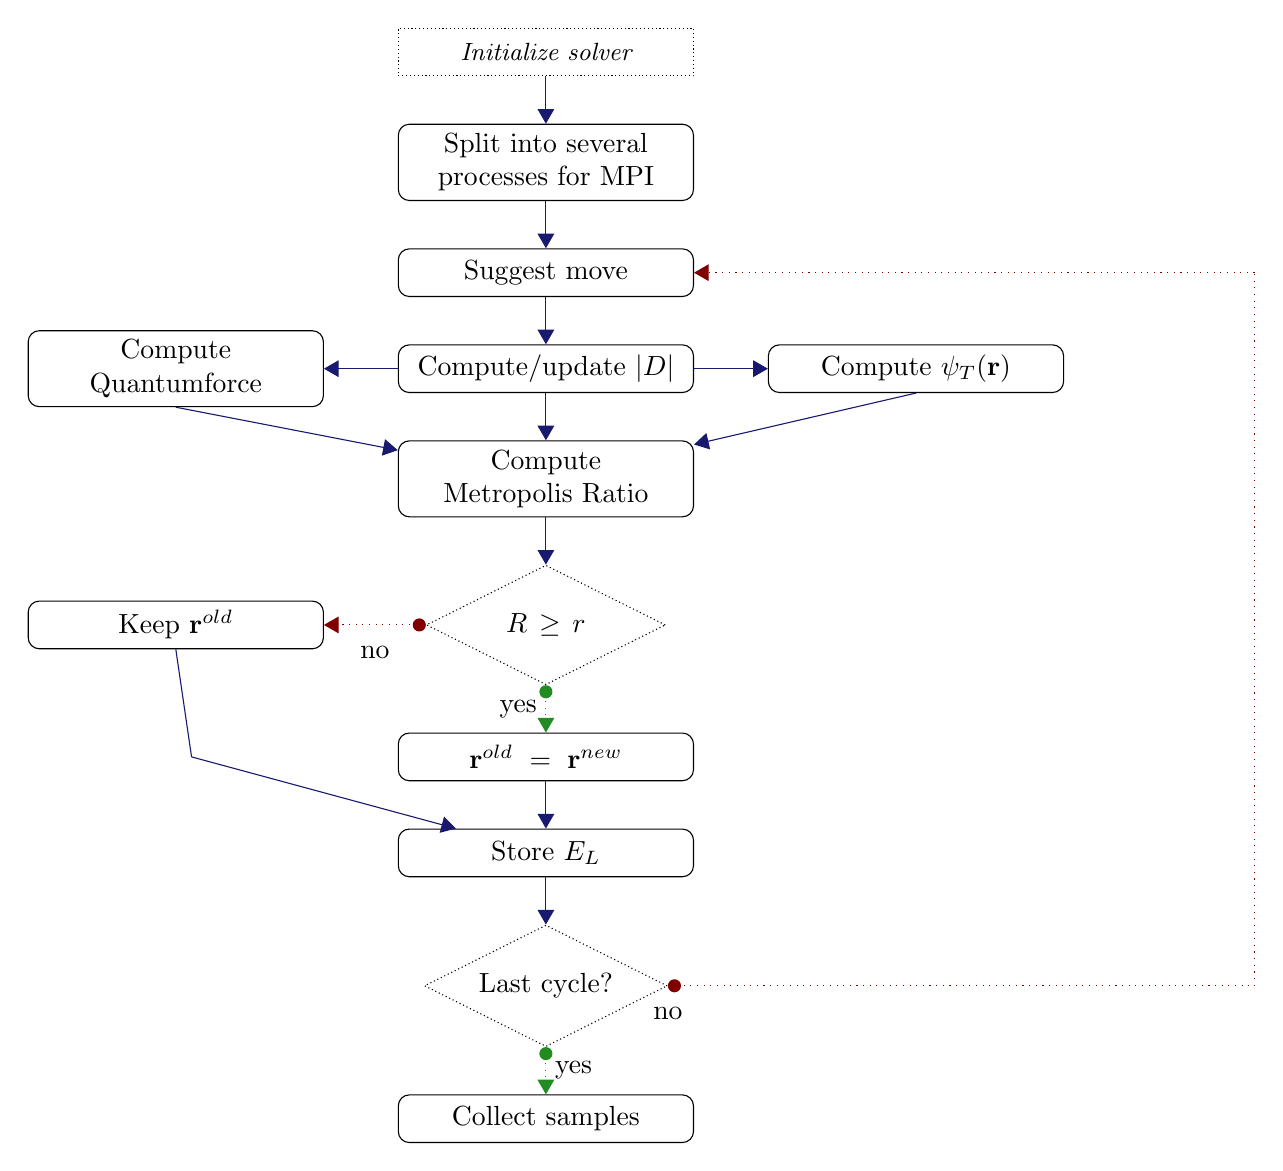
\begin{tikzpicture}[%
		    >=triangle 60,              % Nice arrows; your taste may be different
		    start chain=going below,    % General flow is top-to-bottom
		    node distance=6mm and 47mm, % Global setup of box spacing
		    every join/.style={norm},   % Default linetype for connecting boxes
		    ]
		% ------------------------------------------------- 
		% A few box styles 
		% <on chain> *and* <on grid> reduce the need for manual relative
		% positioning of nodes
		\tikzset{
		  base/.style={draw, on chain, on grid, text centered, minimum height=4ex},
		  proc/.style={base, rectangle, text width=10em},
		  test/.style={base, diamond, aspect=2, text width=5em},
		  term/.style={proc, rounded corners},
		  % coord node style is used for placing corners of connecting lines
		  coord/.style={coordinate, on chain, on grid, node distance=6mm and 45mm},
		  % nmark node style is used for coordinate debugging marks
		  nmark/.style={draw, cyan, circle, font={\sffamily\bfseries}},
		  % -------------------------------------------------
		  % Connector line styles for different parts of the diagram
		  norm/.style={->, draw, lcnorm},
		  free/.style={->, draw, lcfree},
		  cong/.style={->, draw, lccong},
		  it/.style={font={\small\itshape}}
		}
		% -------------------------------------------------
		% Start by placing the nodes
		\node[proc, densely dotted, it] (init) {Initialize solver};
		\node[term, join] (split)      {Split into several processes for MPI};
		\node[term, join] (position)      {Suggest move};
		\node[term, join] (SD) { Compute/update \( |D| \) };
		\node[term, join ] (metro) {Compute Metropolis Ratio};
		\node[test, densely dotted , join ]	(test)	{\(R \ge r\)};
		\node[term]	(new_pos)	{\(\vb{r}^{old} = \vb{r}^{new}\)};
		\node[term, join ]	(energy)	{ Store \(E_L\) };
		\node[test, densely dotted ,join ]	(last)	{Last cycle?};
		\node[term]	(end)	{Collect samples};


		%Setting up the nodes on the side
		\node [term, right=of SD] (trialfunction) {Compute \( \psi_T(\vb{r}) \)};
		\node [term, left=of SD] (quantum) { Compute  Quantumforce};
		\node[term, left=of test] (old_pos) {Keep \(  \vb{r}^{old} \)};
		\node [coord, left=of new_pos] (c1)  {};    
		\node[coord, right=of last]	(around1){};
		\node[coord, right=of around1] (around2) {};
		\node[coord, right=of position]	(around3){};
		\node[coord, right=of around3]	(around4){};


		%Draw new links between boxes
		% \path (SD.south) to node [near start, xshift=1em] {$y$} (quantum);
		\draw [->,lcnorm] (SD.west) -- (quantum);
		\draw [->,lcnorm] (SD.east) -- (trialfunction);
		\draw [->, lcnorm] (quantum.south) -- (metro);
		\draw [->, lcnorm] (trialfunction.south) -- (metro);
		\draw [*->, lccong, , dotted] (test.west) -- (old_pos);
			\path (test.west) to node [ yshift = -1em] {no} (old_pos);
		\draw [*->, lcfree, dotted] (test.south) -- (new_pos);
			\path (test.south) to node [xshift = -1em]{yes} (new_pos);

		\draw [-, lcnorm] (old_pos.south) -- (c1);
		\draw [->, lcnorm] (c1.south) -- (energy);

		\draw[*-, lccong, dotted] (last.east) -- (around2);
			\path (last.east) to node [yshift = -1em] {no} (last);
			\draw[-, lccong, dotted] (around2.east) -- (around4);
			\draw[->, lccong, dotted] (around4) -- (position);

		\draw [*->, lcfree, dotted] (last.south) -- (end);
			\path (last.south) to node [xshift = +1em]{yes} (end);


		\end{tikzpicture}
		\caption{Schematic overview over the workflow of the VMC solver. The solver is initialized and called by the {\tt main}-function.}
		\label{fig:schematic}
	\end{figure}

%\todo{Fix flowcharts.}

\subsection{Class structure}

	Classes in a large program can be many hundred or even thousands of lines long. This makes it messy and cumbersome to keep all classes in a single file. A standard way to deal with this is to have a file for each class and subclass. This is not only much more tidy than having everything in a single file, but has the practical benefit of not needing to recompile the entire program on every compilation; it suffices to compile only the changed classes. This can cut down compilation times considerably.

	\begin{figure}
		\center
		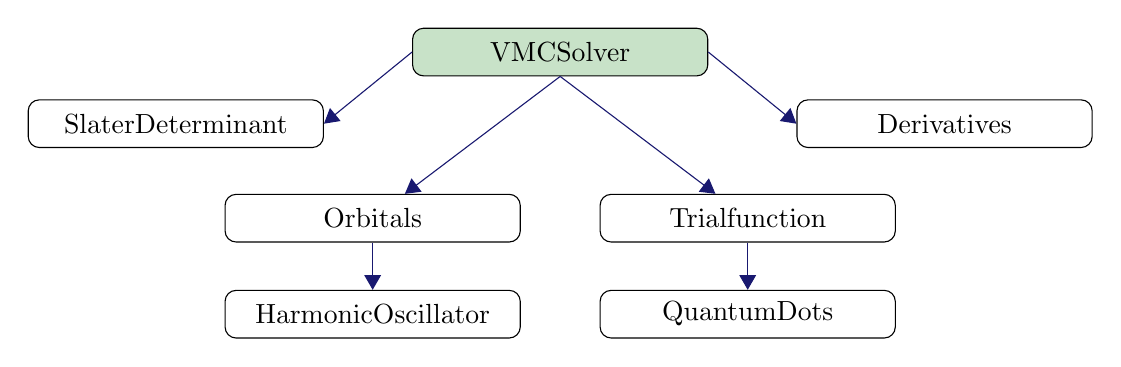
\begin{tikzpicture}[%
			    >=triangle 60,              % Nice arrows; your taste may be different
			    start chain=going below,    % General flow is top-to-bottom
			    node distance=6mm and 35mm, % Global setup of box spacing
			    every join/.style={norm},   % Default linetype for connecting boxes
			    ]
			% ------------------------------------------------- 
			% A few box styles 
			% <on chain> *and* <on grid> reduce the need for manual relative
			% positioning of nodes
			\tikzset{
			  base/.style={draw, on chain, on grid, text centered, minimum height=4ex},
			  proc/.style={base, rectangle, text width=10em},
			  test/.style={base, diamond, aspect=2, text width=5em},
			  term/.style={proc, rounded corners},
			  % coord node style is used for placing corners of connecting lines
			  coord/.style={coordinate, on chain, on grid, node distance=6mm and 45mm},
			  % nmark node style is used for coordinate debugging marks
			  nmark/.style={draw, cyan, circle, font={\sffamily\bfseries}},
			  % -------------------------------------------------
			  % Connector line styles for different parts of the diagram
			  norm/.style={->, draw, lcnorm},
			  free/.style={->, draw, lcfree},
			  cong/.style={->, draw, lccong},
			  it/.style={font={\small\itshape}}
			}

			%Center column
			\node[term, fill=lcfree!25,  text centered] (solver) {VMCSolver};
			\node[coord]	(blank)	{};
			\node[coord]	(empty)	{};
			\node[coord]	(blank2)	{};
			

			% Bottom columns
			\node[term,  right= 0.5 cm and 0.5 cm of blank2] (trialfunction)	{Trialfunction};
				\draw[->, lcnorm]	(solver.south) -- (trialfunction);
			\node[term, join]	(diff)	{QuantumDots}; %{He, Be, Ne, H\(_2\) or Be\(_2\)}

			\node[term,  left= 0.5 cm and 0.5 cm of blank2] (orbitals)	{Orbitals};
				\draw[->, lcnorm]	(solver.south) -- (orbitals);
			\node[term, join]	(HO)	{HarmonicOscillator};

			%Sides with lines drawn
			\node[term, right= 2cm and 3cm of blank] (derivatives) {Derivatives};
				\draw[->, lcnorm] (solver.east) -- (derivatives.west);

			\node[term, left= 2cm and 3cm of blank] 	(slater)	{SlaterDeterminant};
				\draw[->, lcnorm] (solver.west) -- (slater.east);

			%Dotted lines between the connected classes
			%\draw[-, lcfree, densely dotted] (slater.east) -- (derivatives.west);
			%\draw[-, lcfree, densely dotted] (slater.east) -- (trialfunction.north);
			%\draw[-, lcfree, densely dotted] (slater.east) -- (orbitals.north);
			%\draw[-, lcfree, densely dotted] (trialfunction.north) -- (derivatives.west);


		\end{tikzpicture}

		\caption{Class and subclass structure used by the program. The {\tt VMCSolver}-class initializes the other classes {\tt SlaterDeterminant}, {\tt Derivatives}, {\tt Orbitals}, and {\tt Trialfunction}. Classes {\tt Orbitals} and {\tt Trialfunction} each has their own subclasses.}
		\label{fig:classes}
	\end{figure}

			\section{Code}
	
	The VMC solver in this thesis is written in C++. This language is chosen mainly because it is more efficient than high-level languages like Python. It is also especially suitable because of its flexibility as an object-oriented language. To handle matrices efficiently the solver uses the Armadillo library \cite{sanderson2010armadillo}, which provides easy methods for creating and filling matrices and vectors, and doing linear algebra. 

	The main program of the simulator handles running of different tests on the chosen system. To find the optimal values for $\alpha$ and $\beta$ it performs  several simulations over a range of $\alpha$- and $\beta$-values, and iteratively zooms in on the part of the range with the best fit. This way it gains accuracy with each iteration. This can continue until a given accuracy is met, or for a given number of iterations.

	To run tests for different oscillator frequencies the program simply interates over given numbers of electrons and runs simulations with different $\omega$- and $\alpha$-values. 

	\subsubsection{The {\tt VMCSolver}-class}
		At the heart of the simulator is the {\tt VMCSolver} class. During initialization it also initializes the {\tt SlaterDeterminant} class, the {\tt Derivatives} class and the classes containing the harmonic orbitals for two and three dimensions. The main function of the {\tt VMCSolver} class is of course to run the Monte Carlo cycles, where it follows the workflow outlined in Fig. \ref{fig:schematic}.

		The solver starts by setting initial trial positions, and calculating the Slater matrices. 
\begin{lstlisting}[language=C++, firstnumber=134]
	void VMCSolver::runMonteCarloIntegrationIS() {|\Suppressnumber|
	... |\Reactivatenumber{162}|
	//initial trial positions
	for(int i = 0; i < nParticles; i++) {
	  for(int j = 0; j < nDimensions; j++) {
	      rOld(i,j) = GaussianDeviate(&idum)*sqrt(stepLength);
	  }
	}
	//Set up the Slater Matrices after the move
	determinant()->updateSlaterMatrices(rOld,this);
	rNew = rOld;|\Suppressnumber|
	...|\Reactivatenumber{172}|
\end{lstlisting}
		Then it goes into the Monte Carlo cycles loop.
\begin{lstlisting}[language=C++, firstnumber=175]
	for(int cycle = 0; cycle < nCycles; cycle++) {
		//Store the current value of the wave function
     	waveFunctionOld = trialFunction()->waveFunction(rOld, this);
     	derivatives()->numericalGradient(QForceOld,rOld, this);|\Suppressnumber|
		...|\Reactivatenumber{200}|
\end{lstlisting}
		For each iteration we find a new position for the particles, using function for the quantum force.
\begin{lstlisting}[language=C++, firstnumber=200]
for(int i = 0; i < nParticles; i++) {
	for(int j = 0; j < nDimensions; j++) {
	    rNew(i,j) = rOld(i,j) + GaussianDeviate(&idum)*sqrt(stepLength)+QForceOld(i,j)*stepLength*D;
	}|\Suppressnumber|
	...|\Reactivatenumber{205}|
\end{lstlisting}
		To run the Metropolis-Hastings algorithm we first have to compute the ratio of Greens functions
\begin{lstlisting}[language=C++, firstnumber=224]
GreensFunction = 0.0;
for (int j=0; j < nDimensions; j++) {
    GreensFunction += 0.5*(QForceOld(i,j)+QForceNew(i,j))*
      (D*stepLength*0.5*(QForceOld(i,j)-QForceNew(i,j))-rNew(i,j)+rOld(i,j));
}
GreensFunction = exp(GreensFunction);

// The Metropolis test is performed by moving one particle at the time
MHRatio = GreensFunction*(waveFunctionNew*waveFunctionNew) / (waveFunctionOld*waveFunctionOld);
if(ran2(&idum) <= MHRatio) {
    acc_moves += 1;
    for(int j = 0; j < nDimensions; j++) {
        rOld(i,j) = rNew(i,j);
        QForceOld(i,j) = QForceNew(i,j);
        waveFunctionOld = waveFunctionNew;
       	}
      }

      else {
			for(int j = 0; j < nDimensions; j++) {
				rNew(i,j) = rOld(i,j);
				QForceNew(i,j) = QForceOld(i,j);
				determinant()->updateSlaterMatrices(rOld,this);
   		}
   	}|\Suppressnumber|
		...|\Reactivatenumber{252}|
\end{lstlisting}

	After performing the Metropolis test on all the particles, the Monte Carlo cycle is complete. After completing all cycles the energy, variance, and average distances are gathered and written to an outputfile. 


	\subsubsection{The {\tt SlaterDeterminant}-class}
		The class for the Slater determinant has several
                functions. One of its main functions is to update the
                Slater Matrices based on the positions of the
                electrons. This is done by simply calling a function
                of the {\tt Orbitals} class for each element of the
                matrix. The other main function is of course to
                calculate the Slater determinant itself, which it does
                using LU decomposition. The class also contains
                functions to calculate the gradient and the laplacian
                of the Slater determinant. To achieve this we  call the
                functions {\tt get\_gradient} and {\tt get\_laplacian}
                from the {\tt Orbitals} class.

		Calculating the determinant is simplified by splitting
                the Slater determinant by using LU decomposition, as
                found in Ref. \cite{press2007numerical}. This gives us
                two matrices, in the code below named {\tt detUp} and
                {\tt detDown}, from which we can easily find the
                determinant of the Slater matrix.
\begin{lstlisting}[language=C++, firstnumber=167]
double SlaterDeterminantHO::calculateDeterminant(const mat &r,double alpha, VMCSolver *solver){|\Suppressnumber|
	...|\Reactivatenumber{195}|
	ludcmp(detUp, Nhalf, indx, &d1);
	ludcmp(detDown, Nhalf, indx, &d2);

	// compute SD as c00*c11*..*cnn
	SD = 1;
	for (i = 0; i < Nhalf; ++i)
	{
	  SD *= detUp(i, i)*detDown(i, i);
	}
	return d1*d2*SD;
}
\end{lstlisting}
	
	\subsubsection{The {\tt Derivatives}-class}

	In VMC, sampling and updating our matrices efficiently involves calculating a number of derivatives. This is evident in the Quantum Monte Carlo section. To comply with the tidy structure we wish the program to have, the derivatives are grouped in the class {\tt Derivatives}. However, for effiency, some of the derivatives of the orbitals are already calculated, and resides in the {\tt Orbitals}-class. For these, the {\tt Derivatives}-class merely calculates the derivatives based on the precalculated derived functions.

	\subsubsection{The {\tt Orbitals}-classes}
		There are two classes for the harmonic orbitals, one for two dimesions, and one for three dimensions. The functions of the two classes are similar, the only difference is the extra dimension accommodated in the three dimensional version of the class. The functions of the class is exclusively called by the Slater determinant class. The main contents of the class, that is the harmonic oscillator-functions and their derivatives, are generated by a Python script using SymPy. 




	\part{Results}
		\chapter{Results}
			In this chapter results from the calculations will be presented. Results are produced using atomic units, meaning $\hbar = e = m_e = 4\pi \epsilon_0 = 1$, where $m_e$ is the electron mass, and $e_0$ is the vacuum permittivity. 
%\todo{short intro}
			%\input{content/Results/results_Atoms}
			\section{Atoms and Molecules}
	The attention concerning atoms has been on three single atoms, helium, beryllium and neon, and two molecules, dihelium ($\mbox{He}_2$) and diberyllium ($\mbox{Be}_2$). In this section different optimizations of the VMC solver will be tested, and ground state energies and one-body densities will be calculated. There will also be a comparison to calculations using gaussian type orbitals, and a statistical discussion, using blocking.
	
	%\todo{short intro}

	\subsection{Optimization results}
		By using an analytical expression for the local energy instead of using a numerical derivation in the calculation the program becomes more efficient. For Helium we achieve a speedup of nearly 48 percent, while for Beryllium a speedup of approximately 80 percent is achieved, see Table \ref{tab:analyticVSNumeric}.

		\begin{table}
			\center
			\begin{tabular}{ c | c | c | c }
			    %\hline
			   	\textbf{Trialfunction} & Numerical (s) & Analytical (s) & Ratio
			    \\ \hline
			    Helium $\psi_{T}$ & 29.7288 & 20.1189	& 0.6767\tabularnewline
			    %\\	\hline
			    Beryllium $\psi_{T2}$ & 58.9623  &	32.4622 & 0.5505\tabularnewline
				%\\ \hline
			\end{tabular}
			\caption{The time to run a Monte Carlo run with \(10^7\) cycles for Helium, and \(10^6\) cycles for Beryllium. Using an analytical expression for the local energy decreases the computation time by a significant degree for both trialfunctions tested. }
			\label{tab:analyticVSNumeric}
		\end{table}

	\subsection{Speedup with MPI}
		\begin{table}
			\center
			\begin{tabular}{ c | c| c| c| c}
				%\hline
				\textbf{Num. of processes} &	1	&	2	&	3	&	4
				\\ \hline
				Speedup	&	1.0	&	1.97	&	2.90	&	3.35
				%\hline
			\end{tabular}
			\caption{Speedup achieved by using MPI to run computations on multiple processors.}
			\label{tab:MPI_speedup}
		\end{table}

		\begin{figure}
			\centering \includegraphics[width=0.49\linewidth]{content/Results/figures/processor_number_time_comparison}
			\protect\caption{Using MPI, the time used as a function of number of processors used, and the corresponding speedup achieved.}
			\label{fig:MPI_speedup}
		\end{figure}

		It is desirable to have a speedup as close as possible
                to the number of processors used. The speedup measured
                by our VMC program running 1, 2, 3 and 4 processors is shown in
                Table \ref{tab:MPI_speedup} and
                Fig. \ref{fig:MPI_speedup}. We see that the speedup is
                good for 2 and 3 processes, in that it is almost equal
                to the number of processes used. However when running
                4 processes the speedup gain suffers somewhat. This is
                because the computer has only 4 processors, so running
                on all processors the VMC program has to share
                resources with the operating system and other
                programs. However, this simple implementation of our parallel version of the code on standard quad-core PC which can be bought in any supermarket, demonstrates the ease by which Monte Carlo methods can be run in parallel. 

	\subsection{Using brute force Monte Carlo sampling}
		As a first attempt to solve the ground state energy for the helium
		atom we perform Variational Monte Carlo calculation with a brute force
		Metropolis sampling. We do this with two trial wave functions
		\[
		\psi_{T}({\bf r_{1}},{\bf r_{2}},{\bf r_{12}})=\exp{\left(-\alpha(r_{1}+r_{2})\right)}\exp{\left(\frac{r_{12}}{2(1+\beta r_{12})}\right)},
		\]
		using $\alpha$ and $\beta$ as variational parameters. 
		We run the Variational Monte Carlo calculation over
		different values for the two variables $\alpha$ and $\beta$, 
		with $2\times10^{7}$ cycles in the Monte Carlo simulation, and the resulting energies are
		presented in Fig. \ref{fig:HeliumAlphaBeta}.
		
		We find the optimal values to be  $\alpha=1.843$ and $\beta=0.34$, as we can see in the figures.
		Using these values for $\alpha$ and $\beta$ we run the brute force variational Monte Carlo calculation. The program finds an optimal value for the steplength, $\delta$, which results in roughly 50 percent accepted moves. Using $10^{8}$ cycles the algorithm finds the steplength to be $\delta = 1.5$, giving 48.8 percent accepted moves. The energy found with this method is $-2.89024$, with a variance of $3.77402\times10^{-5}$, as presented in Table \ref{tab:Helium_no_IS}.
		The parameter $\alpha$ can be interpreted as a parameter for the
		force pulling the electron to the nucleus.

		\begin{table}
			\center
			%\resizebox{\linewidth}{!}{%
			\begin{tabular}{c|c|c|c}
			    %\hline
			   	Atom  & $\mbox{E}_{\mbox{\scriptsize{VMC}}}$ & Variance & $\mbox{E}_{\mbox{\scriptsize{ref}}}$ \tabularnewline
				\hline 
				Helium & $-2.89024$ & $3.77402\times10^{-5}$ & $-2.9037$ \tabularnewline
				%\hline 
			\end{tabular}%}
			\caption{Ground state energy for Helium calculated with variational Monte Carlo without using Importance Sampling. The reference energy is from Ref. \cite{Binkley_1975}.}
			\label{tab:Helium_no_IS}
		\end{table}
		


		\begin{figure}
			\centering \includegraphics[width=0.49\linewidth]{content/Results/figures/HeliumJastrowAnalytical_alpha_beta_energy}
			\includegraphics[width=0.49\linewidth]{content/Results/figures/HeliumJastrowAnalytical_alpha_beta_variance}
			\protect\caption{For helium using $\psi_{T}$, the energy as a function of alpha and beta (left), and the variance as a function of $\alpha$ and $\beta$. }
			\label{fig:HeliumAlphaBeta}
		\end{figure}

	\subsection{Ground state energies}
		We now introduce importance sampling to our calculations of the Helium atom, and expand the calculations to the Beryllium and the Neon atoms, and the Helium and the Beryllium molecules. 

		%From a search for the optimal variables for Helium, we find them to be $\alpha=1.843$ and $\beta=0.34$. , we get an energy of $-2.89012$ and a corresponding variance $7.76888\times10^{-5}$, 
		Expanding the system to larger atoms, we use the trial functions given in Eq. \eqref{eq:BerylliumTrialFunction} for Beryllium, and Eq. \eqref{eq:NeonTrialFunction} for Neon. Optimal values for $\alpha$ and $\beta$ are found by variation until the ground energy is minimized. The resulting ground state energies of the systems are presented in Table \ref{tab:EnergyAlphaBetaReference}. There is a relatively large uncertainty of the ground state energies, especially for Neon and the molecules, because the variance of the energy compared to the difference in energy caused by varying the parameters is quite high. However, as a function of the variational parameters the variance is more smooth, see fig \ref{fig:HeliumAlphaBeta}, and it is therefore easier to determine the best values for the variables from variance as a function of \(\alpha\) and \(\beta\). The energy and variance as a function of the timestep, $\delta t$ is shown in Fig. \ref{fig:HeliumTimestep}. 

		The ground state energies found with the variational Monte Carlo method are in good agreement with the reference energies. However the method generally underestimates the ground state energies. There is also a big statistical error, increasing with the size of the systems, which stems from a relatively low number of Monte Carlo samples. 


		\begin{figure}
			\centering \includegraphics[width=0.49\linewidth]{content/Results/figures/HeliumJastrowAnalyticalTimeEnergy}
			\includegraphics[width=0.49\linewidth]{content/Results/figures/HeliumJastrowAnalyticalTimeVariance}
			\protect\caption{For helium $\psi_{T}$, timestep shown as a function of energy (left) and variance (right), using $\alpha = 1.84$ and $\beta=0.34$.}
			\label{fig:HeliumTimestep}
		\end{figure}

		\begin{figure}
			\centering\includegraphics[width=0.49\linewidth]{content/Results/figures/Helium_blocking}
			\protect\caption{Statistical analysis for the helium case, using blocking. The blocking behaviour can be seen very clearly as it plateaus rapidly with increasing blocksize.}
			\label{fig:HeliumBlocking}
		\end{figure}


		\begin{figure}
			\centering \includegraphics[width=0.49\linewidth]{content/Results/figures/Beryllium_alpha_beta_energy}
			\centering \includegraphics[width=0.49\linewidth]{content/Results/figures/Beryllium_alpha_beta_variance}
			\protect\caption{Energy (left) and variance (right) as a function of $\alpha$ and $\beta$ for Beryllium, using $10^{6}$ cycles.}
			\label{fig:alpha_beta_comparison_beryllium}
		\end{figure}

		\begin{figure}
			\centering \includegraphics[width=0.49\linewidth]{content/Results/figures/Neon_alpha_beta_energy}
			\centering \includegraphics[width=0.49\linewidth]{content/Results/figures/Neon_alpha_beta_variance}
			\protect\caption{Energy (left) and variance (right) as a function of $\alpha$ and $\beta$ for Neon, using $10^{5}$ cycles.}
			\label{fig:alpha_beta_comparison_neon}
		\end{figure}

		To find optimal $\alpha$ and $\beta$ values for the atoms we
                run VMC with ranges of different values for \(\alpha\)
                and \(\beta\). The resulting plots of the variance and  the
                energy for different combinations are given in
                Fig. \ref{fig:alpha_beta_comparison_beryllium} for
                Beryllium and
                Fig. \ref{fig:alpha_beta_comparison_neon} for Neon. As
                VMC runs slowly for Neon, because it has ten electrons,
                we made runs over the range of Alpha and
                Beta values with $10^{5}$ cycles. This is reflected in
                the higher variance, and the spikes in the variance
                plot.

		\begin{table}
			\center %
			%\resizebox{\linewidth}{!}{%
			\begin{tabular}{c|c|c|c|c}
				%\hline 
				Atom  & $\mbox{E}_{\mbox{\scriptsize{VMC}}}$ & Variance & $\mbox{E}_{\mbox{\scriptsize{ref}}}^{(a)}$ & $\mbox{E}_{\mbox{\scriptsize{ref}}}^{(b)}$ \tabularnewline
				\hline 
				He & $-2.89012$ & $7.77\times10^{-5}$ & $-2.9037$ & $-2.9036(2)$\tabularnewline
				%\hline 
				Be & $-14.3902$  & $9.09\times10^{-4}$ & $-14.667$ & $-14.657(2)$ \tabularnewline
				%\hline 
				Ne  & $-127.875$ & $0.0132$ & $-128.928$ & $-128.765(4)$ \tabularnewline
				%\hline 
				H$_2$ &   $-1.15828$	& $0.00023$  & $-1.17540$ & $-1.1745(3)$ \tabularnewline
				%\hline
				Be$_{2}$   & $ -31.349 $	& $ 0.0076 $  & $-29.339$ & $-29.301(5)$ \tabularnewline
				%\hline
			\end{tabular}%}
			\protect\caption{Ground state energies of atoms and molecules, computed with the variational Monte Carlo method. For H$_2$ and Be$_2$ we used a nuclei distance of \( 1.40 \) and \( 4.63\), respectively.  Refs. (a): \cite{Koput_2011_PCCP} \cite{Binkley_1975}, (b): \cite{hogbergetDMC} (using diffusion Monte Carlo).}
			\label{tab:EnergyAlphaBetaReference} 
			%The binding enery found for Be\(_2\) is too low which is caused by a bug in the implementation of the molecule.
		\end{table}

		\begin{figure}
			\centering \includegraphics[width=0.49\linewidth]{content/Results/figures/Beryllium_blocking}
			\centering \includegraphics[width=0.49\linewidth]{content/Results/figures/Neon_blocking}
			\protect\caption{Statistical analysis of beryllium using blocking with $10^6$ Monte Carlo cycles. There is a clear plateauing behaviour as the blocksize increases after rising dramatically for small blocksizes. This is due to the blocksize catching up to the correlation length between the measurements. \todo{NB!!}}\label{fig01:std_Stuff}
		\end{figure}



	\subsection{Using Gaussian Type Orbitals}
		Using GTOs we can nearly reproduce the energies we get
                from using Slater Type Orbitals, although with GTOs
                not quite as low energies are reached. This is due to
                the GTOs being an imperfect representation of the
                STOs. Using GTOs in stead of STOs is also considerably
                slower, as seen in \ref{tab:AtomsGTO}. This can be due
                to inefficient code, and there is also room for
                improvements by calculating analytical derivatives of
                the GTOs. However using GTOs reduces the variables to
                only $\beta$, thus we don't have to look for energy
                minima by varying $\alpha$. This means that it is
                possible to easily use a gradient method to more
                efficiently find the variable that gives minimum
                energy.

		\begin{table}
			\center %
			\resizebox{\linewidth}{!}{%
			\begin{tabular}{c|c|c|c|c|c|c}
				%\hline 
				Atom &  $\mbox{E}_{\mbox{\scriptsize{VMC}}}$ & Var. & $\mbox{E}_{\mbox{\scriptsize{ref}}}^{(a)}$ & $\mbox{E}_{\mbox{\scriptsize{ref}}}^{(b)}$ & GTO [s] & STO [s] \tabularnewline
				\hline 
				He &  $-2.85482$ & $0.004$ & $-2.9037$ & $-2.9036(2)$ & $15.0$ & $6.5$ \tabularnewline
				%\hline 
				Be  & $-14.0182$ & $0.002$ & $-14.667$ & $-14.657(2)$ & $48321$ & $4141$ \tabularnewline
				%\hline 
				Ne  & $-113.542$ & $0.498$ & $-128.928$ & $-128.765(4)$ & $2821$ & $203$ \tabularnewline
				%\hline 
			\end{tabular}}
			\protect\caption{ Comparison of energies found using bisection method with the refenrence energy \cite{Koput_2011_PCCP} \cite{Binkley_1975} and comparison of the time used running the computation with the given number of cycles using GTOs and STOs.}
			\label{tab:AtomsGTO} 
		\end{table}

	\subsection{One-body densities}
		\subsubsection{Helium Atom}
			Simulations of the helium atom have been
                        studied using several different
                        trialfunctions. First the electrons are
                        regarded as having pure hydrogenlike
                        wavefunctions. Then the hydrogenlike
                        wavefunctions are expanded by optimizing the
                        \(\alpha \) value to get a better ground state
                        energy. For the final calculations the
                        Padé-Jastrow correlation factor is added to
                        include the effects of the electron-electron
                        repulsion. The results of the case without
                        Padé-Jastrow correlation is presented in Table
                        \ref{tab:helium_wavefunctions_tests}. Note
                        that the variance listed is the variance for
                        the local energy between each particle moves in
                        the VMC calculations, not the true variance, which is
                        obtained through the blocking routine
                        described in section \ref{sec:blocking}.

			In Fig. \ref{fig:HeliumoneBodyDensity}
                        histograms of the positions the electrons
                        occupy during the simulations are presented,
                        and we can see that for the pure hydrogenic
                        wavefunction the electrons are generally
                        closer to the nucleus than in the other two
                        simulations. The ground-state energy improved
                        and got closer to the reference value, as
                        listed in \ref{tab:EnergyAlphaBetaReference},
                        as the wavefunction got more sophisticated,
                        and we have a decreasing variance. In the
                        wavefunction the $\alpha$ parameter represents
                        the electrical attraction of the nucleus on
                        the electron, and represents an effective charge.
In a real Helium atom the
                        attraction felt by the electrons is smaller
                        than the charge of the nucleus because it is
                        also under the influence of the other
                        electrons. For the Helium atom the effect of
                        the correlation factor is not very pronounced,
                        because there are only two electrons, and they
                        can be quite far away from each other. However
                        the correlation factor is still significant in
                        the ground-state energy and the variance.

			\begin{table}
			\center %
			%\resizebox{\linewidth}{!}{%
			\begin{tabular}{c|cc}
				%\hline 
				Atom & $\mbox{E}_{\mbox{\scriptsize{VMC}}}$ &Var. \tabularnewline
				\hline 
				He &  $-2.757$ & $0.0030$ \tabularnewline
				Be &  $-13.710$ & $0.0072$ \tabularnewline
				Ne &  $-110.301$ & $0.0477$ \tabularnewline

			\end{tabular}%}
			\protect\caption{ Energies for the helium, beryllium and neon atoms using simple helium wavefunctions with only one variational parameter. Note that the variance is the variance for the local energy between each particle move, not the true variance.}
			\label{tab:helium_wavefunctions_tests} 
			\end{table}

			\begin{figure}
					\centering 
					\includegraphics[width=0.32\linewidth]{content/Results/figures/ChargeDensityHeliumHydrogenic}
					\includegraphics[width=0.32\linewidth]{content/Results/figures/ChargeDensityHeliumSimpleAnalytical}
					\includegraphics[width=0.32\linewidth]{content/Results/figures/ChargeDensityHelium_trimmed}
					\protect\caption{Radial densities of an helium atom simulated with different trial functions. From the left the plots represents pure hydrogenic wave functions, hydrogenic wave functions with an optimized alpha,  and hydrogenic wave functions with a Jastrow factor and optimized variational parameters.}
					\label{fig:HeliumoneBodyDensity}
					% ($\alpha = 2$, $E = -2.757$ and $\sigma^2_* = 0.0030$)
					% ($\alpha = 1.65$, $E = -2.843$ and $\sigma^2_* = 0.0027$)
					% ($\alpha = 1.843$, $\beta = 0.34$, $E = -2.887$, $\sigma^2_* = 0.0010$ )
					%  The simulations were run with \(10^6\) Monte Carlo cycles
			\end{figure}

			As expected, since the trialfunctions used here is based only on the \(\psi_{1S}\) orbitals, the radial distribution is similar to the \(\psi_{1S}\) hydrogen orbital in \ref{fig:orbitals_radial}.


		\subsubsection{Beryllium}
			There is a similar drop in the energy going from a purely hydrogenic wavefunction to a wavefunction where we have introduced a variational parameter, comparing values in Tabs. \ref{tab:helium_wavefunctions_tests} and \ref{tab:EnergyAlphaBetaReference}.
			The hydrogenic wavefunction for Beryllium consists of a Slater determinant constructed of the first two hydrogenic orbitals, plotted in Fig. \ref{fig:orbitals_radial}. The traces of the 1s orbital is there in the first maximum and is closer to the nucleus than in an hydrogen atom, which is expected since the distance is a function of the nucleus charge. The contribution from the second orbital 2s is visible as the second maximum in the distribution of Fig.~\ref{fig:oneBodyDensityBeryllium}. When the correlation factor is included the distribution is smeared out and the orbitals are not as sharply peaked.


			\begin{figure}
				\centering \includegraphics[width=0.49\linewidth]{content/Results/figures/ChargeDensityBerylliumSimple}
				\centering \includegraphics[width=0.49\linewidth]{content/Results/figures/ChargeDensityBeryllium}
				\protect\caption{The radial densities of a beryllium atom simulated with different trial functions. The left plot is with hydrogenic wave functions and the right plot is with hydrogenic wave functions using a Jastrow factor and optimized parameters.}
				\label{fig:oneBodyDensityBeryllium}
				% ($\alpha = 4$, $E = -13.710$, $\sigma^2_* = 0.0072$)
				% ($\alpha = 4$, $\beta = 0.31$,  $E = -14.385$, $\sigma^2_* = 0.0029$ )
			\end{figure}

			
		\subsubsection{Neon}
			As with helium and beryllium there is a drop
                        in the energy as we introduce a variational
                        parameter. The trial functions for neon
                        include all the three orbitals and the
                        distribution, presented in
                        Fig. \ref{fig:oneBodyDensityNeon} is
                        contracted closer to the nucleus than in the
                        other atoms. Here we can see the largest
                        effect due to the inclusion of the correlation
                        factor, both in the ground state energy and
                        the radial distribution. This is because the
                        electrons are closer together than in the
                        other atoms due to the higher charge of the
                        nucleus.
			\begin{figure}
				\centering \includegraphics[width=0.49\linewidth]{content/Results/figures/ChargeDensityNeonSimple}
				\centering \includegraphics[width=0.49\linewidth]{content/Results/figures/ChargeDensityNeon}
				\protect\caption{Radial densities of an Neon atom simulated with different trial functions. The left plot is with hydrogenic wave functions and the right plot is with hydrogenic wave functions with a Jastrow factor and optimized parameters.}
				\label{fig:oneBodyDensityNeon}
				% ($\alpha = 10.22$, $E = -110.301$, $\sigma^2_* = 0.0477$)
				% ( $\alpha = 10.22$, $\beta = 0.0.091$,  $E = -127.888$, $\sigma^2_* = 0.0190$ )
				% The simulations were run with \(10^6\) Monte Carlo cycles
			\end{figure}

		\subsubsection{Hydrogen Molecule}
			Density plots for the hydrogen molecule
                        $H_{2}$ are presented in
                        Fig. \ref{fig:oneBodyDensityHydrogenTwo}. For
                        this molecule, which is comparable to a Helium
                        atom with the protons separated, the radial
                        distribution from the mass center appears
                        slightly more smeared out than in the Helium
                        atom because the protons are slightly apart.
                        In the one-body density plot, sliced about the
                        \(xz\) plane, the electron density around the
                        nuclei is higher. 

			\begin{figure}[H]
				\centering \includegraphics[width=0.32\linewidth]{content/Results/figures/ChargeDensityHydrogenTwo}
				\centering \includegraphics[width=0.32\linewidth]{content/Results/figures/OneBodyDensityHydrogenTwo}
				\centering \includegraphics[width=0.32\linewidth]{content/Results/figures/OneBodyDensityElectronsHydrogenTwo}
				\protect\caption{On the left the the radial distribution of the hydrogen molecule is presented, where both nuclei are placed \(R = 1.40\) atomic units way from each other on the \(z\) axis. In the center a slice of the density in the \(xz\) plane with a width of \(1.0\) atomic units is shown. On the right one-body densities of each of the electrons are shown. Both the nuclei are visible on the one-body density plot as a denser concentration.}
				\label{fig:oneBodyDensityHydrogenTwo}
			\end{figure}



		\subsubsection{Beryllium Molecule}

			For the beryllium molecule, $Be_{2}$, shown in
                        Fig. \ref{fig:oneBodyDensityBerylliumTwo}, the
                        concentration of the one-body density around
                        the nuclei is sharper than in the hydrogen
                        molecule, which is likely caused by the higher
                        charge of the nuclei. In the beryllium atom we
                        also see that the electron density is higher
                        closer to the nucleus. The one-body density
                        plots here are not to be completely trusted
                        because there is a bug in the implementation
                        of the molecule which causes a too low binding
                        energy, but much of the expected physics still
                        seem to be captured by the VMC computation. By
                        following only one of the electrons in the
                        one-body densities presented in
                        Fig. \ref{fig:oneBodyDensityBerylliumTwo} we
                        can see that, compared to the Hydrogen
                        molecule, the nuclei in the molecule trap
                        the  electrons more efficiently.
			
			\begin{figure}[H]
				\centering \includegraphics[width=0.32\linewidth]{content/Results/figures/ChargeDensityBerylliumTwo}
				\centering \includegraphics[width=0.32\linewidth]{content/Results/figures/OneBodyDensityBerylliumTwo}
				\centering \includegraphics[width=0.32\linewidth]{content/Results/figures/OneBodyDensityElectronsBerylliumTwo}
				\protect\caption{On the left the radial distribution of the beryllium molecule is presented, where both nuclei where placed \(R = 4.63\) atomic units away from each other on the \(z\) axis. In the center the one-body density of a slice of density in the the \(xz\) plane with with of \(1.0\) atomic units is shown. On the right one-body densities of each of the electrons is shown. The concentration of the one-body density is very sharp around the two nuclei.}
				\label{fig:oneBodyDensityBerylliumTwo}
			\end{figure}


			\section{Quantum Dots}
	The attention concerning quantum dots has been on studying one-body densities for quantum dots consisting of different magic numbers of electrons, and with different frequencies. Ground state energies have also been calculated, and are compared to energies calculated with other many-body methods. 
	%\todo{short intro}

			\subsection{Verification and validation}
	%\todo{Comment on units ($\hbar = 1$ etc)}

	It is important to test the program, to see if all parts work as intended. This is done by running a simulation of a system of whitch the solution is already known. A great way to test if the program indeed gives the results it should is by testing against a case where there is an exact solution. 

	As a first test we run a simulation where the interaction is neglected. In VMC electron-electron interaction is accounted for by a Coulomb part, and the Jastrow factor. So by ignoring these in our calculations, we can run simulations without interaction. In this case the exact wave function is represented by the trial wave function. The expected energies without interaction are the sum over each occupied orbital, and the energy becomes that of Eq. \eqref{eq:spGroundStateEnergy}.
	%$E_0=\sum^{N} \epsilon_{nm_{l}} = \sum^{N} 2n+\left | m_{l} \right |+1$. 
	%\todo{reference to equation in QD section}

	As we see in Tab. \ref{tab:VMC_no_interaction} the VMC solver yields the expected results. This seemingly simple test actually tests most parts of the VMC machinery. Getting positive results means that vital parts like the {\tt VMCSolver}-class, which runs the Monte Carlo cycles with Metropolis sampling, the class handling the Slater determinant, and the class handling the derivatives all work properly. It also means that the orbitals, generated by a Python script, are implemented correctly. However, as we have neglected the interaction part, some parts are not tested. We therefore need a more thorough test. 
	
	\begin{table}
		\begin{centering}
			\resizebox{\linewidth}{!}{%
			\begin{tabular}{ccccc||ccccc}
				\multicolumn{5}{c||}{2D} & \multicolumn{5}{c}{3D}\tabularnewline
				\hline 
				$\omega$ & N & $\alpha$ & $\mbox{E}_{\mbox{{\scriptsize VMC}}}$ & $\mbox{E}_{0}$ & $\omega$ & N & $\alpha$ & $\mbox{E}_{\mbox{{\scriptsize VMC}}}$ & $\mbox{E}_{0}$\tabularnewline
				\hline 
				$0.5$ & 2 & $1.0$ & $1.0$ & $1$ & $0.5$ & 2 & $1.0$ & $1.5$ & $1.5$ \tabularnewline
				$1.0$ &  & $1.0$ & $2.0$ & $2$ & $1.0$ &  & $1.0$ & $3.0$ & $3$\tabularnewline
				$0.5$ & 6 & $1.0$ & $5.0$ & $5$ & $0.5$ & 8 & $1.0$ & $9.0$ & $9$\tabularnewline
				$1.0$ &  & $1.0$ & $10.0$ & $10$ & $1.0$ &  & $1.0$ & $18.0$ & $18$\tabularnewline
				$0.5$ & 12 & $1.0$ & $14.0$ & $14$ & $0.5$ & 20 & $1.0$ & $30.0$ & $30$\tabularnewline
				$1.0$ &  & $1.0$ & $28.0$ & $28$ & $1.0$ &  & $1.0$ & $60.0$ & $60$\tabularnewline
				$0.5$ & 20 & $1.0$ & $30.0$ & $30$ & $0.5$ & $40$ & $1.0$ & $75.0$ & $75$ \tabularnewline
				$1.0$ &  & $1.0$ & $60.0$ & $60$ & $1.0$ &  & $1.0$ & $150.0$ & $150$ \tabularnewline
				$0.5$ & 30 & $1.0$ & $55.0$ & $55$ & &  &  &  &  \tabularnewline
				$1.0$ &  & $1.0$ & $110.0$ & $110$ & &  &  &  &  \tabularnewline
				$0.5$ & 42 & $1.0$ & $91.0$ & $91$ &  &  &  &  & \tabularnewline
				$1.0$ &  & $1.0$ & $182.0$ & $182$ &  &  &  &  & \tabularnewline
				$0.5$ & 56 & $1.0$ & $140.0$ & $140$ &  &  &  &  & \tabularnewline
				$1.0$ &  & $1.0$ & $280.0$ & $280$ &  &  &  &  & \tabularnewline
				\hline 
			\end{tabular}}
		\par\end{centering}

		\protect\caption{Results from VMC calculations without electron-electron interaction. $N$ is number of particles used in the quantum dot, and $\omega$ is the frequency of the harmonic oscillator. Results for both two dimensional cases and three dimensional cases are tested. For reference the exact energies are given in column $\mbox{E}_{0}$.  \label{tab:VMC_no_interaction}}
	\end{table}

	The next step is to test more parts of the solver by including electron-electron interaction. If we calculate the interaction while ignoring the Jastrow-factor, we should get an energy similar to the energy in the Hartree-Fock case, given by Eq. \eqref{HFenergy_AS}. By neglecting the Jastrow-factor the variational Monte Carlo solver works as a numerical integrator, using the Slater determinant, and the resulting energy is thus an approximation to the energy which can be calculated manually with Eq. \eqref{HFenergy_AS}. The results are presented in Tab. \ref{tab:VMCnoJ_vs_HF}. With the exception of the two-particle case, all the energies calculated with VMC without the Jastrow-factor are slightly higher than then ones calculated using Hartree-Fock. However they are all very close to the HF-energies, which is what was required.

	\begin{table}[h]
		\begin{centering}
			\begin{tabular}{ccc}
				N & $E_{VMC}$ & $E_{HF}$ \tabularnewline
				\hline
				2 & 3.17151 & 3.25331 \tabularnewline
				6 & 20.8133 & 20.71922 \tabularnewline
				12 & 67.1167 & 66.91132 \tabularnewline
				20 & 158.446 & 158.0043 \tabularnewline
			\end{tabular}
		\par\end{centering}
		\protect\caption{Energies computed with VMC without the Jastrow-factor compared to the Hartree-Fock energies calculated with Eq. \eqref{HFenergy_AS}. \label{tab:VMCnoJ_vs_HF}}
	\end{table}

	The remaining part of the solver is the inclusion of electron-electron correlation in the calculations. Correlations are implemented with the so-called Jastrow-factor in the trialfunction, which relies on parts of the derivatives-, orbitals-, and Slater determinant-classes. As we now include correlations in our calculations, there is no way to analytically calculate the resulting energy. Therefore we have to check our results against other, independent calculations of the same system as refenrence. 
			\subsection{Ground state energies}
	
	Ground state energies of quantum dots are presented in table \ref{tab:QD_ground_state}. They are compared to results from similar studies using diffusion Monte Carlo, Similarity Renormalization Group Theory, Coupled Cluster singles and doubles, and full configuration interaction.

	The energies calculated are generally higher than the energies presented from similar studies. This can be due to the fact that the variational Monte Carlo method is unable to reach as low energies and the same accuracy as for example diffusion Monte Carlo or the other methods presented. Another source for the error may be insufficiency in the search for optimal variational parameters because of limited time and resources, especially for quantum dots consisting of a higher number of electrons. Nonetheless, the energies found using the variational Monte Carlo method are in fairly good agreement with the reference energies.  

	A case where the variational Monte Carlo method does better than the reference is against the full configuration interaction for 12 and 20 electrons. This is due to the number of shells above the highest filled shell used in the FCI calculations, which are low in these cases, leading to inaccurate results.

	For low number of electrons in the quantum dot we see that the energies are in good agreement with the references, with results accurate to up to two decimals for the two-electron case. However the error grows with increasing number of electrons in the system. 

	%\todo{mer kommentering av energiene}

	Next we look at the ratio between the potential and kinetic energy as a function of $\hbar\omega$. The ratios are presented in Fig. \ref{fig:TV_ratio}. Unfortunately the results here are somewhat jumpy, despite using plenty of Monte Carlo cycles. However it still shows that when we lower the frequency, $\omega$, the ratio breaks down, and the potential energy becomes dominating. With lower frequency the electrons no longer possess as much kinetic energy, and the repulsive forces makes the potential energy the predominant energy.  
	%\todo{flytte?}

	%\todo{3D}
	
	\begin{table}[H]
		\begin{centering}
			\resizebox{\linewidth}{!}{%
			\begin{tabular}{cc|cccccc}
				N  & $\omega$  & $\mbox{E}_{\mbox{{\scriptsize VMC}}}$  & $\mbox{E}_{ref}^{(a)}$  & $\mbox{E}_{ref}^{(b)}$  & $\mbox{E}_{ref}^{(c)}$  & $\mbox{E}_{ref}^{(d)}$\tabularnewline
				\hline 
				2  & $0.01$  & 0.0797255(1) & -  & 0.0738\{23\}  & 0.07373505 \{19\}  & 0.073839(2)\tabularnewline
				& $0.1$  & 0.45156772(1) & -  & 0.4408\{23\}  & 0.44079191 \{19\}  & 0.44079(1)\tabularnewline
				& $0.28$  & 1.0264107(2) & 0.99263\{19\}  & 1.0217\{23\}  & 1.0216441 \{19\}  & 1.02164(1)\tabularnewline
				& $0.5$  & 1.6633891(2) & 1.643871\{19\}  & 1.6599\{23\}  & 1.6597723 \{19\}  & 1.65977(1)\tabularnewline
				& $1.0$  & 3.0010648(3) & 2.9902683\{19\}  & 3.0002\{23\}  & 3.0000001 \{19\}  & 3.00000(1)\tabularnewline
				\hline 
				6  & $0.1$  & 3.6712647(1) & 3.49991 \{18\} & 3.5805 \{22\}  & 3.551776 \{9\}  & 3.55385(5)\tabularnewline
				 & $0.28$  & 7.7496318(1) & 7.56972 \{18\} & 7.6254\{22\}  & 7.599579\{6\}  & 7.60019(6)\tabularnewline
				 & $0.5$  & 11.956646(2) & 11.76228 \{18\} & 11.8055 \{22\} & 11.785915 \{6\} & 11.78484(6)\tabularnewline
				 & $1.0$  & 20.376948(2) & 20.14393 \{18\} & 20.1734 \{22\} & 20.160472 \{8\} & 20.15932(8)\tabularnewline
				\hline 
				12  & $0.1$  & 12.568683(1) & 12.2253 \{17\} & 12.3497 \{21\} & 12.850344 \{3\} & 12.26984(8)\tabularnewline
				 & $0.28$  & 26.056874(1) & 25.61084 \{17\} & 25.7095\{21\}  & 26.482570 \{2\} & 25.63577(9)\tabularnewline
				 & $0.5$  & 39.684993(2) & 39.13899 \{17\} & 39.2194 \{21\} & 39.922693 \{2\} & 39.1596(1)\tabularnewline
				 & $1.0$  & 66.660247(2) & 65.68304 \{17\} & 65.7399 \{21\} & 66.076116 \{3\} & 65.7001(1)\tabularnewline
				\hline 
				20  & $0.1$  & 33.959997(1) & 29.95345 \{16\} & 30.2700 \{8\} & 34.204867 \{1\} & 29.9779(1)\tabularnewline
				 & $0.28$  & 62.958144(1) & 61.91368 \{16\} & 62.0676\{20\}  & 67.767987 \{1\} & 61.9268(1)\tabularnewline
				 & $0.5$  & 95.405501(1) & 93.86145 \{16\} & 93.9889 \{20\} & 100.93607 \{1\} & 93.8752(1)\tabularnewline
				 & $1.0$  & 158.4896(2) & 155.8665 \{16\} & 155.9569 \{20\} & 164.61280 \{1\} & 155.8822(1)\tabularnewline
				\hline 
				% 1545.914()
				% 113.24424()
				30  & $0.1$  & - & 60.43000 \{15\} & 61.3827\{9\}  & -  & 60.4205(2)\tabularnewline
				 & $0.28$   & - & 123.9733 \{15\} & 124.2111\{9\}  & -  & 123.9683(2)\tabularnewline
				 & $0.5$  & 194.11612(1) & 187.0408 \{15\} & 187.2231 \{19\} & -  & 187.0426(2)\tabularnewline
				 & $1.0$  & 313.26857(2) & 308.5536 \{15\} & 308.6810 \{19\} & -  & 308.5627(2)\tabularnewline
				\hline 
				%42  & $0.1$  &  & -  & 111.7170 \{8\} & -  & 107.6389(2)\tabularnewline
				% & $0.28$  &  & 219.8836 \{14\} & 222.1401 \{8\} & -  & 219.8426(2)\tabularnewline
				% & $0.5$  &  & 330.6485 \{14\} & 331.8901 \{8\} & -  & 330.6306(2)\tabularnewline
				% & $1.0$  &  & 542.9528 \{14\} & 543.1155 \{18\} & -  & 542.9428(8)\tabularnewline
				%\hline 
				%56  & $0.1$  &  & -  & 186.1034 \{9\} & -  & 175.9553(7)\tabularnewline
				% & $0.28$  &  & -  & 363.2048 \{9\} & -  & 358.145(2)\tabularnewline
				% & $0.5$  &  & -  & 540.3430 \{9\} & -  & 537.353(2)\tabularnewline
				% & $1.0$  &  & -  & 879.6386 \{17\} & -  & 879.3986(6)\tabularnewline
				%\hline 
			\end{tabular}}
	\par\end{centering}

	\protect\caption{Ground state results for $N$-electron quantum dots in two dimensions, with frequency $\omega$. Refs. (a): \cite{reimannSRGT} (using Similarity Renormalization Group Theory), (b): \cite{hirthCC} (using Coupled Cluster singles and doubles), (c): \cite{olsenFCI} (using full configuration interaction), (d): \cite{hogbergetDMC} (using diffusion MC). Numbers in curly brackets represent the number of shells above the highest filled shell, referred to as the Fermi-level \cite{shavitt09}, which has been used to construct the basis.\label{tab:QD_ground_state}}
	\end{table}

\begin{figure}[H]
	\begin{centering}
		\includegraphics[width=1.0\linewidth]{Misc/gen_figs/KinPotPlotMulti}
		
	\par\end{centering}

	\protect\caption{Ratio of $\left\langle T\right\rangle /\left\langle V\right\rangle $, that is the ratio of the expectation value for the kinetic energy and the expectation value for the potential energy,
	for quantum dots consisting of 2, 6, 12, and 20 electrons. \label{fig:TV_ratio}}
\end{figure}

\newcolumntype{Y}{>{\centering\arraybackslash}>{\hsize=.5\hsize}X}
\newcolumntype{P}{>{\raggedleft\arraybackslash}X}
\begin{table}[H]
	\begin{centering}
		\begin{tabularx}{\textwidth}{YY|PPP}
		N  & $\omega$  & $\mbox{E}_{\mbox{{\scriptsize VMC}}}$  & $\mbox{E}_{ref}^{(a)}$  & $\mbox{E}_{ref}^{(b)}$ \\
		\hline 
		2  & $0.1$  & 0.5033689(2) & 0.5 & 0.499997(3) \\
		 & $0.28$  & 1.2037916(2) & - & 1.201725(2)\\
		 & $0.5$  & 2.0018226(2) & 2.0 & 2.000000(2)\\
		 & $1.0$  & 3.7355844(3) & - & 3.730123(3)\\
		\hline 
		8  & $0.1$  & 5.7612847(1) & - & 5.7028(1)\\
		 & $0.28$  & 12.320225(2) & - & 12.1927(1)\\
		 & $0.5$  & 19.043405(2) & - & 18.9611(1)\\
		 & $1.0$  & 33.317234(2) & - & 32.6680(1)\\
		\hline 
		20  & $0.1$ &  27.603613(1) & - & 27.2717(2)\\
		 & $0.28$ &  56.829274(2) & - & 56.3868(2)\\
		 & $0.5$  & 86.667247(2) & - & 85.6555(2)\\
		 & $1.0$  & 145.13357(2) & - & 142.8875(2)\\
		\hline 
		%40  & $0.1$  &  & - & -\\
		% & $0.28$  &  & - & -\\
		% & $0.5$  &  & - & -\\
		% & $1.0$  &  & - & -\\
		%\hline 
		\end{tabularx}
	\end{centering}

	\caption{Ground state results for $N$-electron quantum dots in three dimensions,
	with frequency $\omega$. Refs. (a): \cite{taut1993two} (using analytical solutions) (b): \cite{hogbergetDMC} (using diffusion Monte Carlo).}\label{tab:QD_ground_state_3D}
\end{table}

%\todo{kommentar om 3D energier}
Ground state energies for quantum dots in three dimensions are presented in table \ref{tab:QD_ground_state_3D}. Quantum dot systems in three dimensions are less studied than their two-dimension counterpart, and as such there are less reference energies to test against. We see however, against the reference energies listed, that as with the two-dimensional cases the ground state energies computed with the variational Monte Carlo method are in fairly good agreement with the reference energies, but are generally higher. With a two-particle system the energies are accurate to two decimal places compared to the references, which is in agreement with the indicated accuracy. However the gap between the computed energy and the reference energies grows with the number of electrons in the system.


\subsection{One-body densities}
	In Fig. \ref{fig:radial_densities} the radial one-body densities for some of the quantum dots are presented. For the two-particle case there is a single peak, slightly smeared with increasing radius. For six particles the distribution is more smeared and the peak is shifted to a higher radius, because of the inclusion of a second filled shell. We see in the 12, 20, and 30 particle cases that the peaks are shifted further with the inclusion of more filled shells. Thus, as more shells are filled, the density distribution gains extrema points. 

	Additionally the densities without Coulomb interaction are shown. For two particles the difference is small as effects from interaction are minimal with so few particles. However it shows a slightly sharper peak for the non-interacting case. As we add more filled shells we see that the same effect, and with more particles the effect becomes more pronounced. Removing the Coulomb force from the calculations thus makes the distribution become more localized and shifted towards the center, due to the reduced potential energy between the energies, meaning that the electrons can be situated closer together.

	%\todo{yukawa}
	To study the importance of the Coulomb forces in the interaction, a factor $e^{-\mu r}$ is introduced, where $\mu$ is a constant. This is called the Yukawa interaction, named after its creator \cite{yukawa1935interaction}. With this modified interaction the reach of the Coulomb force, which usually is virtually infinite, is killed off by the exponential factor. Looking at the difference in Fig. \ref{fig:yukawa_interaction} it is evident that the density is shifted towards the center when using the Yukawa factor. Because the Coulomb interaction is killed off for larger distances, each particle no longer feels as strong repulsive force from the other electrons. They can thus be closer together, as the density shows.

	\begin{figure}
		\begin{centering}
			\subfloat[$N=2$]{\begin{centering}
			\includegraphics[width=0.49\linewidth]{Misc/gen_figs/noInter/QD2_2D_1_densityplot_both}
			\par\end{centering}

			\centering{}}\subfloat[$N=6$]{\begin{centering}
			\includegraphics[width=0.49\linewidth]{Misc/gen_figs/noInter/QD6_2D_1_densityplot_both}
			\par\end{centering}

			\centering{}}
			\par\end{centering}

			\begin{centering}
			\subfloat[$N=12$]{\begin{centering}
			\includegraphics[width=0.49\linewidth]{Misc/gen_figs/noInter/QD12_2D_1_densityplot_both}
			\par\end{centering}

			\centering{}}\subfloat[$N=20$]{\begin{centering}
			%\includegraphics[width=0.49\linewidth]{Misc/gen_figs/20/QD20_2D_1_densityplot.png}
			\includegraphics[width=0.49\linewidth]{Misc/gen_figs/noInter/QD20_2D_1_densityplot_both}
			\par\end{centering}

			\centering{}}
			\par\end{centering}

			\begin{centering}
			\subfloat[$N=30$]{\begin{centering}
			%\includegraphics[width=0.49\linewidth]{Misc/gen_figs/20/QD20_2D_1_densityplot.png}
			\includegraphics[width=0.49\linewidth]{Misc/gen_figs/noInter/QD30_2D_1_densityplot_both}
			\par\end{centering}

			\centering{}}
			\par\end{centering}

		\protect\caption{Radial one-body densities of quantum dots in two dimensions, consisting of 2, 6, 12, 20, and 30 particles, with and without electron-electron interaction. \label{fig:radial_densities}}

	\end{figure}

\begin{figure}
		\begin{centering}
			\includegraphics[width=0.6\linewidth]{Misc/gen_figs/noInter/QD6_2D_0.01_densityplot_yukawa2}
		\par\end{centering}
\protect\caption{Radial one-body density of a two-dimensional quantum dot consisting of six particles and frequency $\omega=0.01$, with and without a Yukawa factor in the Coulomb interaction. \label{fig:yukawa_interaction}}

	\end{figure}

	One-body densities for quantum dots in two dimensions with a frequency $\omega=1$ are presented in Fig. \ref{fig:oneB_dens_w1}. It is easy to see how the densities correspond to the radial densities. There is a single peak in the center in the two particle case, corresponding to the single filled shell. Meanwhile in the six particle case there is no peak in the center, but a ring of high density surrounding the center, corresponding to the single peak in the radial density. Another such ring can be seen in the 12 particle case, together with a high density in the center. There is a clear pattern emerging, with a wavelike behaviour with increasing numbers of filled shells. The high density center in the two electron case can thus be seen in the 12 electron case, which again can be seen in the center of the 30 electron case (although the center in the 30 electron case is not as defined). The same can also be seen for the six and 20 particle cases. This similar shape in the middle is a result of the systems being in energetically favourable configurations. 

	One-body densities for lower frequencies, presented in Fig. \ref{fig:oneB_dens_table}, shows similar shapes, but with larger radial size. As we lower the frequency, the radial size grows. For the $\omega=0.1$ cases the one-body densities for higher number of particles does not exhibit as clear wave-like shapes anymore due to a limited number of samplings in the calculations. 

	An interesting feature arising in the one-body densities is that for very low frequencies the densities change structure. In the two-particle case, with $\omega=0.01$, there is no longer a peak in the middle, the one-body density resembles more the six-particle case with a decreased density in the center. Similarly in the six-particle case with $\omega=0.01$ there is a peak in the center, unlike for higher frequencies, making it resemble the 12-particle case.

	It is evident from the one-body densities that lowering the frequencies makes the density more smeared out, from the increasing size as frequency is lowered. The density thus becomes more even and more localized as the frequency is lowered, which suggests that the electrons are, on average, more evenly spread across the shell structure. This interpretation is further supported by Fig. \ref{fig:TV_ratio}, where we see the ratio between the kinetic and potential energy break down as the frequency is lowered, suggesting that the potential energy becomes dominating.
	%\todo{mer kommentering}

	%\todo{kommenter 3D densities}
	In three dimensions the one-body densities, presented in Fig. \ref{fig:oneB_dens_w1_3D}, are evidently quite similar to their two-dimensional counterparts, exhibiting the same wave-like distribution of the density. However the similarity only holds for the same number of closed shells, meaning that for example the 8 particle case in three dimensions corresponds to the 6 particle case in two dimensions, as presented in Fig. \ref{fig:oneB_dens_w1}, because they both have two filled shells. 

	Comparing two and three dimensions it is therefore clear that for two particles we have a single peak in both dimensions, for 6 particles in two dimensions and 8 in three dimensions we have a single band of high density surrounding a low point, and for 12 particles in two dimensions and 20 in three dimensions we have a peak in the center and a band of high density surrounding it.

	%\todo{eksempel på lavere frekvens med 3D}
	With a very low frequency, $\omega=0.01$, it is from Fig. \ref{fig:oneB_dens_table} evident that the density becomes localized and that the particles gets evenly distributed over the shells. That is, for example for a very low frequency for the six particle case, the shape containing a single band of high density shows an elevated density in the center, from the lowest filled shell. Looking at an example for the three dimensional case, Fig. \ref{fig:oneB_dens_w001_3D}, also with two filled shells and a frequency of $\omega=0.01$, the same effect apparently does not apply in three dimensions; there are no signs of an elevated density in the center. We thus get a breaking of symmetry.

	For low frequencies in two dimensions, where the density becomes localized and evenly distributed in shells, it is apparent that the quantum dots become crystallized in what is called a Wigner crystal, named after Wigner who predicted them \cite{wigner1934interaction}. This effect is expected for the quantum dots for low electron densities, where the potential energy dominate over the kinetic energy \cite{Landman07}. 

	%\todo{virial theorem}
	It is clear that the quantum dots form Wigner crystals caused by the relationship between the kinetic and potential energy. The relationship between the kinetic and potential energy is related to what in classical mechanics is known as the virial theorem. For quantum mechanical systems the virial theorem gives the relation between the kinetic and potential energy operators, $\hat{\mathbf{T}}$ and $\hat{\mathbf{V}}$, with the relation
	
	\begin{equation}
		\hat{\mathbf{V}}(\mathbf{r}) \propto r^{\gamma} \rightarrow \langle \hat{\mathbf{T}} \rangle = \frac{\gamma}{2} \langle \hat{\mathbf{V}} \rangle,
	\end{equation}
	
	first shown by Fock \cite{fock1930bemerkung}. Thus two systems which have the same ratio of kinetic to potential energy will follow the same effective potential and similar eigenstates.
	\clearpage


	\begin{figure}[H]
	\begin{centering}
		\subfloat[$N=2$]{\begin{centering}
		\includegraphics[width=0.49\linewidth]{Misc/gen_figs/2/QD2_2D_1_OneBodyDensityplot_cropped}
		\par\end{centering}

		\centering{}}\subfloat[$N=6$]{\begin{centering}
		\includegraphics[width=0.49\linewidth]{Misc/gen_figs/6/QD6_2D_1_OneBodyDensityplot_cropped}
		\par\end{centering}

		\centering{}}
		\par\end{centering}

		\begin{centering}
		\subfloat[$N=12$]{\begin{centering}
		\includegraphics[width=0.49\linewidth]{Misc/gen_figs/12/QD12_2D_1_OneBodyDensityplot_cropped}
		\par\end{centering}

		\centering{}}\subfloat[$N=20$]{\begin{centering}
		\includegraphics[width=0.49\linewidth]{Misc/gen_figs/20/QD20_2D_1_OneBodyDensityplot_cropped}
		\par\end{centering}

		\centering{}}
		\par\end{centering}

		\begin{centering}
		\subfloat[$N=30$]{\begin{centering}
		\includegraphics[width=0.49\linewidth]{Misc/gen_figs/30/QD30_2D_1_OneBodyDensityplot_cropped}
		\par\end{centering}
		\centering{}}
		\par\end{centering}

	\protect\caption{One-body density with $\omega = 1.0$ \label{fig:oneB_dens_w1}}

	\end{figure}

\begin{figure}[H]
	\begin{centering}
		\subfloat[One-body densities for $N=2$]{\begin{centering}
		\begin{tabular}{ccc}
			\includegraphics[width=0.3\linewidth]{Misc/gen_figs/2/QD2_2D_0.28_OneBodyDensityplot_cropped} & 
			\includegraphics[width=0.3\linewidth]{Misc/gen_figs/2/QD2_2D_0.1_OneBodyDensityplot_cropped} &
			\includegraphics[width=0.3\linewidth]{Misc/gen_figs/2/QD2_2D_0.01_OneBodyDensityplot_cropped} 
			\tabularnewline
		$\omega=0.28$ & $\omega=0.1$ & $\omega=0.01$\tabularnewline
		\end{tabular}
		\par\end{centering}

		}
	\par\end{centering}

	\begin{centering}
		\subfloat[One-body densities for $N=6$]{\begin{centering}
		\begin{tabular}{ccc}
			\includegraphics[width=0.3\linewidth]{Misc/gen_figs/6/QD6_2D_0.28_OneBodyDensityplot_cropped} & 
			\includegraphics[width=0.3\linewidth]{Misc/gen_figs/6/QD6_2D_0.1_OneBodyDensityplot_cropped} &
			\includegraphics[width=0.3\linewidth]{Misc/gen_figs/6/QD6_2D_0.01_OneBodyDensityplot_cropped} 
			\tabularnewline
		$\omega=0.28$ & $\omega=0.1$ & $\omega=0.01$\tabularnewline
		\end{tabular}
		\par\end{centering}

		}
	\par\end{centering}

	\begin{centering}
		\subfloat[One-body densities for $N=12$]{\begin{centering}
		\begin{tabular}{ccc}
			\includegraphics[width=0.3\linewidth]{Misc/gen_figs/12/QD12_2D_0.5_OneBodyDensityplot_cropped} & 
			\includegraphics[width=0.3\linewidth]{Misc/gen_figs/12/QD12_2D_0.28_OneBodyDensityplot_cropped} & 
			\includegraphics[width=0.3\linewidth]{Misc/gen_figs/12/QD12_2D_0.1_OneBodyDensityplot_cropped}  
			\tabularnewline
		$\omega=0.5$ & $\omega=0.28$ & $\omega=0.1$\tabularnewline
		\end{tabular}
		\par\end{centering}

		}
	\par\end{centering}

	\begin{centering}
		\subfloat[One-body densities for $N=20$]{\begin{centering}
		\begin{tabular}{ccc}
			\includegraphics[width=0.3\linewidth]{Misc/gen_figs/20/QD20_2D_0.5_OneBodyDensityplot_cropped} & 
			\includegraphics[width=0.3\linewidth]{Misc/gen_figs/20/QD20_2D_0.28_OneBodyDensityplot_cropped} & 
			\includegraphics[width=0.3\linewidth]{Misc/gen_figs/20/QD20_2D_0.1_OneBodyDensityplot_cropped}  
			\tabularnewline
		$\omega=0.5$ & $\omega=0.28$ & $\omega=0.1$\tabularnewline
		\end{tabular}
		\par\end{centering}

		}
	\par\end{centering}

	\protect\caption{One-body densities for different $\omega$-values \label{fig:oneB_dens_table}}
\end{figure}

\begin{figure}[H]
	\begin{centering}
		\subfloat[$N=2$]{\begin{centering}
			\includegraphics[width=0.49\linewidth]{Misc/gen_figs/2/QD2_3D_1_OneBodyDensityplot3D_cropped}
			\includegraphics[width=0.49\linewidth]{Misc/gen_figs/2/QD2_3D_1_densityplot_cropped}
		\par\end{centering}

		}
	\par\end{centering}
	\begin{centering}
		\subfloat[$N=8$]{\begin{centering}
			\includegraphics[width=0.49\linewidth]{Misc/gen_figs/8/QD8_3D_1_OneBodyDensityplot3D_cropped}
			\includegraphics[width=0.49\linewidth]{Misc/gen_figs/8/QD8_3D_1_densityplot_cropped}
		\par\end{centering}
		}
	\par\end{centering}

	\begin{centering}
		\subfloat[$N=20$]{\begin{centering}
		\includegraphics[width=0.49\linewidth]{Misc/gen_figs/20/QD20_3D_1_OneBodyDensityplot3D_cropped}
		\includegraphics[width=0.49\linewidth]{Misc/gen_figs/20/QD20_3D_1_densityplot_cropped}
		\par\end{centering}
		}

	\par\end{centering}

	\protect\caption{One-body densities of quantum dots in three dimensions, consisting of 2, 8, and 20 electrons, with frequency $\omega=1$. One eight of the density-sphere has been removed to reveal the distribution of density to the center. The radial density distribution for each case is also presented on the right.  \label{fig:oneB_dens_w1_3D}}


\end{figure}

\begin{figure}
	\begin{centering}
		\includegraphics[width=0.49\linewidth]{Misc/gen_figs/8/old backup/QD8_3D_0.01_OneBodyDensityplot3D_cropped}
		\includegraphics[width=0.49\linewidth]{Misc/gen_figs/8/QD8_3D_0.01_densityplot_cropped}
	\par\end{centering}

	\protect\caption{One-body density of a three-dimensional quantum dot consisting of 8 electrons, with  frequency $\omega=0.01$. One eight of the density-sphere has been removed to reveal the distribution of density to the center. On the right the corresponding radial density is shown. \label{fig:oneB_dens_w001_3D}}


\end{figure}
		\chapter{Conclusion}
		In this chapter, we have developed three many-body methods we will use throughout this thesis. The most fundamental of these methods is the Hartree-Fock theory, which will recover a reasonable amount of the system's energy. It is an independent particle model, so it cannot account for the energy from interacting particles. The first post-Hartree-Fock method we developed, so-called because it improves the Hartree-Fock result, was many-body perturbation theory (MBPT) which provides a convenient truncation scheme that allows for systematic improvements to the Hartree-Fock results. The final many-body method, developed in great detail due to its importance later in this thesis, was coupled cluster theory, which is more accurate than MBPT but much more time-consuming. Coupled cluster theory also provides a convenient truncation scheme and, at the triple level, allows us to recover most of the system's energy even with the method being truncated. Now that we have developed our many-body methods, the next chapter will be devoted to developing the system to which these methods will be applied: infinite matter.
	
	\begin{appendices}
		
\chapter{Closed expression for noncorrelation Helium trialfunction}
	\label{sec:helium_noncorrelating}
	\section{Derivation of local energies, using radial coordinates}
		The local energy of is dependant on the Hamiltonian and the wavefunction describing the system, the Hamiltonian incorporates both a kinetic energy part given by \( \frac{\nabla_i^2}{2} \) for each particle
		and a potential energy part given by \(\frac{Z}{r_i}\) and \(\frac{1}{r_{ij}}\), where \(Z\) is the charge of the center, \(r_i\) is the distance for electron \(i\) to the atom center and \(r_{ij}\) is the distance between electron \(l\) and \(m\). Then the local energy is given by the following:

		\begin{align}
			E_L &= \sum_{i,i<j}{\frac{1}{ \Psi_T(\vb{r_i} , \vb{r_{ij}}) } \hat{H} \Psi_T(\vb{r_i} , \vb{r_{ij}})}
			\\
			&=	\sum_{i,i<j}\frac{1}{ \Psi_T(\vb{r_i} , \vb{r_{ij}}) } \left( - \frac{\nabla_i^2}{2} -\frac{Z}{r_i}  -  \frac{Z}{r_j} +  \frac{1}{r_{ij} }  \right) \Psi_T(\vb{r_i} , \vb{r_{ij}})
			\\
			&= \sum_{i,i<j}{-\frac{1}{2\Psi_T} \left(\nabla_i^2 \Psi_T  \right)  -\frac{Z}{r_i}  -  \frac{Z}{r_j} +  \frac{1}{r_{ij} }}
		\end{align}

		Let us change derivation variables:

		\begin{align}
			-\frac{1}{2\Psi_T} \left(\nabla_i^2 \Psi_T  \right) &= \sum_{m=1}^{3}{-\frac{1}{2\Psi_T} \left( \pdv[2]{\Psi_T}{x_m} \right)_i}
			\\
			&= \sum_{m=1}^{3}{-\frac{1}{2\Psi_T} \left( \pdv{}{x_m} \left( \pdv{\Psi_T}{r_i}\pdv{r_i}{x_m} \right) \right)_i}
			\intertext{Since \(r_i = \left( x_1^2 + x_2^2 + x_3^2 \right)^{1/2}\) then \( \pdv{r_i}{x_m} = \pdv{\left( x_1^2 + x_2^2 + x_3^2 \right)^{1/2}}{x_m} =\frac{x_m}{r_i} \)}
			&= \sum_{m=1}^{3}{-\frac{1}{2\Psi_T} \left( \pdv{}{x_m} \left( \pdv{\Psi_T}{r_i}\frac{x_m}{r_i} \right) \right)_i}
			\\
			&= \sum_{m=1}^{3}{-\frac{1}{2\Psi_T} \left( \pdv{\Psi_T}{x_m}{r_i}\frac{x_m}{r_i} + \pdv{\Psi_T}{r_i} \pdv{}{x_m} \left(\frac{x_m}{r_i} \right) \right)_i}
			\intertext{ The term \( \pdv{}{x_m} \left(\frac{x_m}{r_i} \right) \) becomes for the different values for \(m\),  \(\pdv{}{x_1}  \left( \frac{x_1}{\left( x_1^2 + x_2^2 + x_3^2 \right)^{1/2}} \right) = \frac{x_2^2 + x_3^2}{r_i^3}\) so all the values for \(m\) term it should sum up to \( \frac{ 2 (x_1^2 + x_2^2 + x_3^2) }{ r_i^3 } \) }
			&= -\frac{1}{2\Psi_T} \left( \pdv[2]{\Psi_T}{r_i}\frac{x_1^2 + x_2^2 + x_3^2}{r^2_i} + \pdv{\Psi_T}{r_i} \frac{ 2 (x_1^2 + x_2^2 + x_3^2) }{ r_i^3 } \right)_i
			\\
			&= -\frac{1}{2\Psi_T} \left( \pdv[2]{\Psi_T}{r_i} + \pdv{\Psi_T}{r_i} \frac{ 2 }{ r_i } \right)
		\end{align}
		Then the local energy becomes:
		\begin{align}
			E_L = \sum_{i,i<j}{  -\frac{1}{2\Psi_T} \left( \pdv[2]{\Psi_T}{r_i} + \pdv{\Psi_T}{r_i} \frac{ 2 }{ r_i } \right)  -\frac{Z}{r_i}  -  \frac{Z}{r_j} +  \frac{1}{r_{ij} }} \label{eq:He_localEnergy}
		\end{align}

		We can apply this to the simple helium trialfunction with no electronic interaction to obtain the local energy.

		\subsubsection{Helium: Simple trialfunction}
		The simple version of the trial function is only dependant on one parameter \( \alpha \) and does not take into account interaction between the two electrons, it is of the form
		\[ \Psi_T (\vb{r_1}, \vb{r_2}) = \exp{ -\alpha (r_1 + r_2) } \]Let us set this trialfunction into the equation for the local energy \eqref{eq:He_localEnergy}. 
		\begin{align}
			E_L &= \sum_{i,i<j}{  -\frac{1}{2\Psi_T} \left( \pdv[2]{e^{-\alpha (r_i + r_j)}}{r_i} + \pdv{e^{-\alpha (r_i + r_j)}}{r_i} \frac{ 2 }{ r_i } \right)  -\frac{Z}{r_i}  -  \frac{Z}{r_j} +  \frac{1}{r_{ij} }}
			\\
			E_L &= -\frac{1}{2\Psi_T} \sum_{i=1}^2{ \left( \alpha^2 -\alpha \frac{ 2 }{ r_i } \right) \Psi_T  -\frac{Z}{r_i} +  \frac{1}{r_{ij} } }
			\\
			E_L &= -\alpha^2 + (\alpha-Z) \left( \frac{1}{r_1} + \frac{1}{r_2} \right) + \frac{1}{r_{12}} \label{eq:heliumLocalEnergy}
		\end{align}

\chapter{GTO constants}
\label{sec:GTO_app}
	In the following tables of constants used to combine the contracted Gaussian type orbitals for Helium, Beryllium, and Neon are presented.

	\begin{table}[H]
		\begin{centering}
			\begin{tabular}{|c|}
				\hline 
				1s\tabularnewline
				\hline 
				0.4579\tabularnewline
				\hline 
				0.6573\tabularnewline
				\hline 
			\end{tabular}
		\par\end{centering}
		\caption{Constants for combining contracted GTOs for Helium. \label{tab:GTO_constants_He}}
	\end{table}

	\begin{table}[H]
		\begin{centering}
			\begin{tabular}{|c|c|}
			\hline 
			1s  & 2s\tabularnewline
			\hline 
			-9.9281e-01  & -2.1571e-01\tabularnewline
			\hline 
			-7.6425e-02  & 2.2934e-01\tabularnewline
			\hline 
			2.8727e-02  & 8.2235e-01\tabularnewline
			\hline 
			1.2898e-16  & 5.1721e-16\tabularnewline
			\hline 
			-2.3257e-19  & 4.5670e-18\tabularnewline
			\hline 
			5.6097e-19  & -1.1040e-17\tabularnewline
			\hline 
			1.2016e-16  & 8.5306e-16\tabularnewline
			\hline 
			-4.6874e-19  & 7.0721e-18\tabularnewline
			\hline 
			1.1319e-18  & -1.7060e-17\tabularnewline
			\hline 
		\end{tabular}
		\par\end{centering}
		\caption{Constants for combining contracted GTOs for Beryllium. \label{tab:GTO_constants_Be}}
	\end{table}

	\begin{table}[H]
		\begin{centering}
			\resizebox{\linewidth}{!}{%
			\begin{tabular}{|c|c|c|c|c|}
			\hline 
			1s  & 2s  & $2p_{x}$  & $2p_{y}$  & $2p_{z}$\tabularnewline
			\hline 
			-9.8077e-01  & -2.6062e-01  & 1.1596e-16  & -8.3716e-18  & -1.9554e-17\tabularnewline
			\hline 
			-9.3714e-02  & 2.5858e-01  & -2.0106e-16  & -9.7173e-17  & -7.3738e-17\tabularnewline
			\hline 
			2.2863e-02  & 8.1619e-01  & -3.2361e-16  & 1.3237e-16  & 1.5789e-16\tabularnewline
			\hline 
			-9.9519e-19  & -5.6186e-18  & 2.7155e-02  & -4.0320e-01  & 3.9171e-01\tabularnewline
			\hline 
			-1.2125e-18  & -2.8615e-16  & -5.6207e-01  & -2.5833e-02  & 1.2375e-02\tabularnewline
			\hline 
			-4.1800e-19  & 4.6199e-17  & 9.1139e-03  & -3.9180e-01  & -4.0392e-01\tabularnewline
			\hline 
			-1.6696e-19  & -4.2405e-18  & 2.8890e-02  & -4.2895e-01  & 4.1673e-01\tabularnewline
			\hline 
			1.2125e-18  & -2.9426e-16  & -5.9797e-01  & -2.7482e-02  & 1.3166e-02\tabularnewline
			\hline 
			3.8779e-19  & 5.0519e-17  & 9.6959e-03  & -4.1683e-01  & -4.2972e-01\tabularnewline
			\hline 
		\end{tabular}}
		\par\end{centering}
		\caption{Constants for combining contracted GTOs for Neon. \label{tab:GTO_constants_Ne}}
	\end{table}


		\chapter{Harmonic oscillator orbitals in two dimensions}
	\label{sec:HOO_2D}
	Harmonic oscillator orbitals in two dimensions are a combination of hermite polynomials of the $x$-coordinate, hermite polynomials of the $y$-coordinate, and an exponential factor. The orbitals are thus created as
	\[
		\phi(\mathbf{r})_{n_{x},\,n_{y}}=H_{n_{x}}(kx)H_{n_{y}}(ky)e^{-\frac{1}{2}k^{2}r^{2}}.
	\]
	Here $k=\sqrt{\omega\alpha}$, where $\omega$ is the oscillator frequency and $\alpha$ is the variational parameter. In the following the hermite polynomials and resulting orbitals will be listed. \clearpage

	\begin{table}[H]
	\begin{centering}
		%\resizebox{\linewidth}{!}{%
		\begin{tabular}{c|l}
			$H_{0}(kx)$ & $1$  \tabularnewline
			$H_{1}(kx)$ & $2kx$  \tabularnewline
			$H_{2}(kx)$ & $4k^2x^2-2$  \tabularnewline
			$H_{3}(kx)$ & $8k^3x^3-12x$  \tabularnewline
			$H_{4}(kx)$ & $16k^4x^4-48k^2x^2+12$  \tabularnewline
			$H_{5}(kx)$ & $32k^5x^5-160k^3x^3+120$  \tabularnewline
			$H_{6}(kx)$ & $64k^6x^6-480k^4x^4+720k^2x^2-120$  \tabularnewline
			\hline
			$H_{0}(ky)$ & $1$  \tabularnewline
			$H_{1}(ky)$ & $2ky$  \tabularnewline
			$H_{2}(ky)$ & $4k^2y^2-2$  \tabularnewline
			$H_{3}(ky)$ & $8k^3y^3-12y$  \tabularnewline
			$H_{4}(ky)$ & $16k^4y^4-48k^2y^2+12$  \tabularnewline
			$H_{5}(ky)$ & $32k^5y^5-160k^3y^3+120$  \tabularnewline
			$H_{6}(ky)$ & $64k^6y^6-480k^4y^4+720k^2y^2-120$ \tabularnewline
		\end{tabular}%}
	\par\end{centering}
	\protect\caption{Hermite polynomials used to create the harmonic oscillator orbitals in two dimensions.}
	\end{table}

	\input{../SymPy/generated_latex/gen_tex_orb}

\chapter{Harmonic oscillator orbitals in three dimensions}
	\label{sec:HOO_3D}
	Harmonic oscillator orbitals in three dimensions are a combination of hermite polynomials of the $x$-coordinate, hermite polynomials of the $y$-coordinate, hermite polynomials of the $z$-coordinate, and an exponential factor. The orbitals are thus created as
	\[
		\phi(\mathbf{r})_{n_{x},\,n_{y},\,n_{z}}=H_{n_{x}}(kx)H_{n_{y}}(ky)H_{n_{z}}(kz)e^{-\frac{1}{2}k^{2}r^{2}}.
	\]
	Here $k=\sqrt{\omega\alpha}$, where $\omega$ is the oscillator frequency and $\alpha$ is the variational parameter. In the following the hermite polynomials and resulting orbitals will be listed. \clearpage

	\begin{table}[H]
	\begin{centering}
		%\resizebox{\linewidth}{!}{%
		\begin{tabular}{c|l}
			$H_{0}(kx)$ & $1$  \tabularnewline
			$H_{1}(kx)$ & $2kx$  \tabularnewline
			$H_{2}(kx)$ & $4k^2x^2-2$  \tabularnewline
			$H_{3}(kx)$ & $8k^3x^3-12x$  \tabularnewline
			\hline
			$H_{0}(ky)$ & $1$  \tabularnewline
			$H_{1}(ky)$ & $2ky$  \tabularnewline
			$H_{2}(ky)$ & $4k^2y^2-2$  \tabularnewline
			$H_{3}(ky)$ & $8k^3y^3-12y$  \tabularnewline
			\hline
			$H_{0}(kz)$ & $1$  \tabularnewline
			$H_{1}(kz)$ & $2kz$  \tabularnewline
			$H_{2}(kz)$ & $4k^2z^2-2$  \tabularnewline
			$H_{3}(kz)$ & $8k^3z^3-12z$  \tabularnewline
		\end{tabular}%}
	\par\end{centering}
	\protect\caption{Hermite polynomials used to create the harmonic oscillator orbitals in three dimensions.}
	\end{table}

	\input{../SymPy/generated_latex/gen_tex_orb_3d}

	\end{appendices}

	\bibliography{bibliography}
	\bibliographystyle{apalike}

\end{document}
